\documentclass[a4paper,oneside,12pt]{book}

\usepackage[usenames,dvipsnames]{xcolor}

%% === nezbytné balíčky:
\usepackage{lmodern}
% \usepackage[T1]{fontenc}    % kódování písma
%\usepackage[IL2]{fontenc}  % kódování písma

\usepackage[utf8]{inputenc}     % vstupní znaková sada tohoto dokumentu: UTF-8
%\usepackage[cp1250]{inputenc}  % vstupní znaková sada tohoto dokumentu: Windows 1250
%\usepackage[latin2]{inputenc}  % vstupní znaková sada tohoto dokumentu: ISO Latin 2

\usepackage[czech]{babel} % česky psaná práce, typografická pravidla. Překládejte pomocí "latex.exe" nebo "pdflatex.exe"
%\usepackage{czech} % česky psaná práce. Překládejte pomocí "pdfCSlatex.exe" ("cslatex.exe" asi bude mít problém s balíkem geometry)

\usepackage[a4paper, hmarginratio=3:2]{geometry} % využití A4 stránky a nastavení okrajů (u vazby bude širší)

\usepackage{pdfpages} % pokud nemáte formulář "Zadání bak./dipl. práce" naskenovaný jako PDF, tak ZAKOMENTUJTE
\usepackage[hidelinks]{hyperref} % v PDF budou klikací odkazy ("hidelinks" je nebude rámovat)

%% === balíčky, které se mohou hodit:
%\usepackage{encxvlna} % postará se o spojky a předložky, které dle českých pravidel nesmí být na konci řádku. Dokumentace: http://texdoc.net/texmf-dist/doc/generic/encxvlna/encxvlna.pdf (chová se správně k "vnitřku" listings?)

\usepackage{graphicx} % balíček pro vkládání rastrových grafických souborů (PNG apod.)
%\usepackage{epsfig} % balíčky pro vkládání grafických souborů typu EPS
% \usepackage{float} % rozšířené možnosti umístění obrázků
% \restylefloat{table}
\usepackage{pifont}
\newcommand{\cmark}{\text{\ding{51}}}
\newcommand{\xmark}{\text{\ding{55}}}
%\usepackage{caption} % pro popisky obrázků, tabulek atd.

\usepackage{tabularx} % rozšířené možnosti tabulek
\usepackage{longtable}
\usepackage{booktabs}
\usepackage{makecell}

\renewcommand{\listfigurename}{Seznam obrázků}
\renewcommand{\listtablename}{Seznam tabulek}
\renewcommand{\arraystretch}{1.3}
\usepackage[font=small]{caption}

% \usepackage{tabu} % jiný balík pro rozšířené možnosti tabulek

\usepackage{listings}

\lstset{upquote=true}

\definecolor{codegreen}{rgb}{0,0.6,0}
\definecolor{codegray}{rgb}{0.7,0.7,0.7}
\definecolor{codepurple}{rgb}{0.58,0,0.82}
\definecolor{backcolour}{rgb}{0.98,0.98,0.98}
\newcommand\numberstyle[1]{%
    \tiny
    \color{codegray}%
    \ttfamily
    \ifnum#1<10 0\fi#1%
}


\lstdefinestyle{mystyle}{
    backgroundcolor=\color{backcolour},   
    commentstyle=\color{codegreen},
    keywordstyle=\color{codepurple},
    numberstyle=\numberstyle,
    stringstyle=\color{codepurple},
    basicstyle=\footnotesize\ttfamily,
    breakatwhitespace=false,
    breaklines=true,
    captionpos=b,
    keepspaces=true,
    numbers=left,
    numbersep=8pt,
    showspaces=false,
    showstringspaces=false,
    showtabs=false,
    frame=none,
    linewidth=1.05\textwidth}


\lstset{style=mystyle}
% \lstset{style=mystyle}  % balíček vhodný pro ukázky zdrojového kódu v~textu práce/příloh. Nutno nastavit! http://ftp.cvut.cz/tex-archive/macros/latex/contrib/listings/listings.pdf
% \usepackage[autoload=true]{jlcode}
% \lstset{language=Python}

\usepackage{amsmath,amsfonts,amssymb}

% \usepackage{color} % pro možnost barevného textu
%\usepackage{fancybox} % umožňuje pokročilé rámečkování
\usepackage{url}
\usepackage{bm}
\usepackage{hyperref}
\usepackage{threeparttable}
%\usepackage{index} % nutno použít v případě tvorby rejstříku balíčkem makeindex
%\newindex{default}{idx}{ind}{Rejstřík} % zavádí rejstřík v případě použití balíku index
\usepackage{csquotes}
\MakeOuterQuote{"}

\frenchspacing % za větou bude mezislovní mezera (v anglických textech je mezera za větou delší)
\widowpenalty=1000 % "síla" zákazu vdov (= jeden řádek ze začátku odstavce na konci stránky)
\clubpenalty=1000 % "síla" zákazu sirotků (= jeden řádek/slovo z konce odstavce samostatně na začátku stránky)
\brokenpenalty=1000 % "síla" zákazu zlomu stránky za řádkem, který má na konci rozdělené slovo

\topmargin=-15mm      % horní okraj trochu menší
\textwidth=150mm      % šířka textu na stránce
\textheight=240mm     % "výška" textu na stránce


\pagenumbering{arabic} % číslování stránek arabskými číslicemi
\pagestyle{plain}      % stránky číslované dole uprostřed

\parindent=0pt % odsazení 1. řádku odstavce
\parskip=7pt   % mezera mezi odstavci

%% --- zde jsou zavedeny některé "konstanty" - některé musíte změnit! --- %%
\newcommand{\cvut}{České vysoké učení technické v~Praze}
\newcommand{\fjfi}{Fakulta jaderná a fyzikálně inženýrská}
\newcommand{\ksi}{Katedra softwarového inženýrství}
\newcommand{\km}{Katedra matematiky}
\newcommand{\program}{Aplikace přírodních věd} % změňte, pokud máte jiný stud. program
\newcommand{\obor}{Aplikace informatiky v přírodních vědách} % změňte, pokud máte kurzívujiný obor

\newcommand{\druh}{Diplomová práce} % nebo "Diplomová práce"
\newcommand{\woman}{a} % pokud jste ŽENA, ZMĚŇTE na: ...{\woman}{a} (je to do Prohlášení)

\newcommand{\logoCVUT}{
\includegraphics{symbol_cvut_konturova_verze_cb.pdf}} % logo ČVUT -- podle grafického manuálu ČVUT platného od prosince 2016. Pokud nevyhovuje PDF-verze, tak použijte jinou variantu loga: https://www.cvut.cz/logo-a-graficky-manual -> "Symbol a logo ČVUT v Praze"). Pokud chcete logo úplně vynechat, zadejte místo "\includegraphics{...}" text "\vspace{35mm}"

% přesně podle formuláře "Zadání bak./dipl. práce" VYPLŇTE:
\newcommand{\nazevczT}{Analýza příčin vzniku shrinku produktů společnosti na základě logistických dat}    % český název práce (přesně podle zadání!)
\newcommand{\nazevenT}{Root Cause Analysis of Shrinkage Based on Logistics Data}          % anglický název práce (přesně podle zadání!)
\newcommand{\nazevcz}{Analýza příčin vzniku shrinku produktů společnosti na základě logistických dat}    % český název práce (přesně podle zadání!)
\newcommand{\nazeven}{Root Cause Analysis of Shrinkage Based on Logistics Data}          % anglický název práce (přesně podle zadání!)
\newcommand{\autor}{Bc. Anna Radová}   % vyplňte své jméno a příjmení (s akademickým titulem, máte-li jej)
\newcommand{\vedouci}{Ing. Martin Plajner, Ph.D.} % vyplňte jméno a příjmení vedoucího práce, včetně titulů, např.: Doc. Ing. Ivo Malý, Ph.D.
\newcommand{\pracovisteVed}{Oddělení matematické teorie rozhodování, Ústav teorie informace a automatizace AV ČR, v.v.i.} % ZMĚŇTE, pokud vedoucí Vaší práce není z KSI
\newcommand{\konzultant}{--} % POKUD MÁTE určeného konzultanta, NAPIŠTE jeho jméno a příjmení
\newcommand{\pracovisteKonz}{--} % POKUD MÁTE konzultanta, NAPIŠTE jeho pracoviště

% podle skutečnosti VYPLŇTE:
\newcommand{\rok}{2023}  % rok odevzdání práce (jen rok odevzdání, nikoli celý akademický rok!)
\newcommand{\kde}{Praze} % studenti z Děčína ZMĚNÍ na: "Děčíně" (doplní se k "prohlášení")

\newcommand{\klicova}{Datová analýza, Logistika}   % zde NAPIŠTE česky max. 5 klíčových slov
\newcommand{\keyword}{Data Analysis, Logistics}       % zde NAPIŠTE anglicky max. 5 klíčových slov (přeložte z češtiny)
\newcommand{\abstrCZ}{}

% zde NAPIŠTE abstrakt v češtině (cca 7 vět, min. 80 slov)
\newcommand{\abstrEN}{} % zde NAPIŠTE abstrakt v angličtině

\newcommand{\prohlaseni}{Prohlašuji, že jsem svou bakalářskou práci vypracoval\woman{} samostatně a použil\woman{} jsem pouze podklady (literaturu, projekty, SW atd.) uvedené v přiloženém seznamu.} % text prohlášení můžete mírně upravit :-)

\newcommand{\podekovani}{Chtěla bych poděkovat doktoru Ing. Martinu Plajnerovi, Ph.D. za vedení mé diplomové práce, za cenné rady, připomínky a trpělivost během tvorby této práce a za čas strávený touto pomocí. Dále děkuji své rodině a manželovi za obrovkou podporu při psaní práce a během celého studia.} % NAPIŠTE poděkování, např. svému vedoucímu:
% Děkuji Ing. Eleonoře Krtečkové, Ph.D. za vedení mé bakalářské práce a za podnětné návrhy, které ji obohatily.
% NEBO:
% Děkuji vedoucímu práce doc. Pafnutijovi Snědldítětikaši, Ph.D. za neocenitelné rady a pomoc při tvorbě bakalářské práce.

\newcommand{\ti}{\textit} % zkrácený příkaz pro kurzívu
\newcommand{\tb}{\textbf} % zkrácený příkaz pro tučné písmo
\newcommand{\tn}{\texttt} % zkrácený příkaz pro neproporcionalni písmo


% Vzhled kódu
\renewcommand{\lstlistingname}{Kód}
%New colors defined below
\definecolor{julia}{rgb}{0.12,0.6,0.08}
\definecolor{julia}{rgb}{0.12,0.6,0.08}
\definecolor{chromeyellow}{rgb}{1.0, 0.65, 0.0}
\definecolor{byzantine}{rgb}{0.74, 0.2, 0.64}
\definecolor{airforceblue}{rgb}{0.36, 0.54, 0.66}
\definecolor{backcolor}{rgb}{0.95,0.95,0.95}
\definecolor{border}{rgb}{0.98,0.98,0.98}

% Takhle se pouziva pro ukazky kodu
% \begin{lstlisting}[caption=Definice metody size pro dataset Iris, label=Kod:ImSiz]
%     size(::Iris) = (150, 0, 0)
% \end{lstlisting}

% napise julia> barevne
\newcommand{\jul}{\textcolor{julia}{julia> }}


\newenvironment{repl}
{\fontfamily{cmvtt}\selectfont \begin{mdframed}

}{\end{mdframed}}

\usepackage[linewidth=1pt]{mdframed}


\newcolumntype{L}{>{\centering\arraybackslash}m{2cm}}
\newcolumntype{N}{>{\centering\arraybackslash}m{1.7cm}}
\newcolumntype{M}{>{\centering\arraybackslash}m{1.6cm}}
\newcolumntype{K}{>{\centering\arraybackslash}m{1.5cm}}
\newcolumntype{S}{>{\centering\arraybackslash}m{1cm}}
\renewcommand{\arraystretch}{1.3}

\newcommand{\cmark}{\textcolor{green!80!black}{\ding{51}}}
\newcommand{\xmark}{\textcolor{red}{\ding{55}}}




% Listing style
\lstdefinelanguage{julia}
{%
%
% julia's keywords:
%
morekeywords=[1]
{%
abstract type,baremodule,begin,break,catch,ccall,const,continue,do,else,elseif,%
end,export,finally,for,function,global,if,import,in,isa,let,local,macro,module,%
mutable struct,primitive type,quote,return,struct,try,using,where,while, function%
},%
%
% julia's literals:
%
morekeywords=[2]
{%
ARCH,ARGS,Apr,April,Aug,August,BINDIR,CPU_NAME,CPU_THREADS,C_NULL,DEPOT_PATH,%
DL_LOAD_PATH,Dec,December,ENDIAN_BOM,ENV,Feb,February,Fri,Friday,I,%
ISODateFormat,ISODateTimeFormat,ISOTimeFormat,Inf,Inf16,Inf32,Inf64,%
InsertionSort,JIT,Jan,January,Jul,July,Jun,June,KERNEL,LOAD_PATH,MACHINE,Mar,%
March,May,MergeSort,Mon,Monday,NaN,NaN16,NaN32,NaN64,Nov,November,Oct,October,%
PROGRAM_FILE,QuickSort,RFC1123Format,RTLD_DEEPBIND,RTLD_FIRST,RTLD_GLOBAL,%
RTLD_LAZY,RTLD_LOCAL,RTLD_NODELETE,RTLD_NOLOAD,RTLD_NOW,RoundDown,%
RoundFromZero,RoundNearest,RoundNearestTiesAway,RoundNearestTiesUp,RoundToZero,%
RoundUp,STDLIB,Sat,Saturday,Sep,September,Sun,Sunday,Thu,Thursday,Tue,Tuesday,%
VERSION,WORD_SIZE,Wed,Wednesday,catalan,devnull,dlext,e,eulergamma,false,%
golden,im,missing,nothing,pi,stderr,stdin,stdout,true,undef,γ,π,φ,ℯ%
},%
%
% julia's built-ins:
%
morekeywords=[3]
{%
AbstractArray,AbstractChannel,AbstractChar,AbstractDict,AbstractDisplay,%
AbstractFloat,AbstractIrrational,AbstractLogger,AbstractMatrix,AbstractREPL,%
AbstractRNG,AbstractRange,AbstractSerializer,AbstractSet,AbstractSparseArray,%
AbstractSparseMatrix,AbstractSparseVector,AbstractString,AbstractUnitRange,%
AbstractVecOrMat,AbstractVector,AbstractWorkerPool,Adjoint,Any,ArgumentError,%
Array,AssertionError,Atomic,Base64DecodePipe,Base64EncodePipe,BasicREPL,%
Bidiagonal,BigFloat,BigInt,BitArray,BitMatrix,BitSet,BitVector,Bool,%
BoundsError,BroadcastStyle,BunchKaufman,CachingPool,CapturedException,%
CartesianIndex,CartesianIndices,Cchar,Cdouble,Cfloat,Channel,Char,Cholesky,%
CholeskyPivoted,Cint,Cintmax_t,Clong,Clonglong,ClusterManager,Cmd,CodeInfo,%
CodeInstance,Colon,Complex,ComplexF16,ComplexF32,ComplexF64,CompositeException,%
Condition,ConsoleLogger,Cptrdiff_t,Cshort,Csize_t,Cssize_t,Cstring,Cuchar,%
Cuint,Cuintmax_t,Culong,Culonglong,Cushort,Cvoid,Cwchar_t,Cwstring,DataType,%
Date,DateFormat,DatePeriod,DateTime,Day,DenseArray,DenseMatrix,DenseVecOrMat,%
DenseVector,Diagonal,Dict,DimensionMismatch,Dims,DivideError,DomainError,%
EOFError,Eigen,Enum,ErrorException,Event,Exception,ExponentialBackOff,Expr,%
FDWatcher,FILE,Factorization,FileMonitor,Float16,Float32,Float64,FolderMonitor,%
Function,Future,GeneralizedEigen,GeneralizedSVD,GeneralizedSchur,GenericArray,%
GenericDict,GenericOrder,GenericSet,GenericString,GitConfig,GitRepo,GlobalRef,%
GotoNode,HMAC_CTX,HTML,Hermitian,Hessenberg,Hour,IO,IOBuffer,IOContext,%
IOStream,IPAddr,IPv4,IPv6,IdDict,IndexCartesian,IndexLinear,IndexStyle,%
InexactError,InitError,Int,Int128,Int16,Int32,Int64,Int8,Integer,%
InterruptException,InvalidStateException,Irrational,KeyError,LAPACKException,%
LDLt,LQ,LU,LinRange,LineEditREPL,LineInfoNode,LineNumberNode,LinearIndices,%
LoadError,LogLevel,LowerTriangular,MIME,Matrix,MersenneTwister,Method,%
MethodError,MethodInstance,Microsecond,Millisecond,Minute,Missing,%
MissingException,Module,Month,NTuple,NamedTuple,Nanosecond,NewvarNode,Nothing,%
NullLogger,Number,OrdinalRange,OutOfMemoryError,OverflowError,Pair,%
PartialQuickSort,Period,PermutedDimsArray,PhiCNode,PhiNode,PiNode,Pipe,%
PollingFileWatcher,PosDefException,ProcessExitedException,%
ProcessFailedException,Ptr,QR,QRPivoted,QuoteNode,RandomDevice,%
RankDeficientException,Rational,RawFD,ReadOnlyMemoryError,Real,ReentrantLock,%
Ref,Regex,RegexMatch,RemoteChannel,RemoteException,RoundingMode,SHA1_CTX,%
SHA224_CTX,SHA256_CTX,SHA2_224_CTX,SHA2_256_CTX,SHA2_384_CTX,SHA2_512_CTX,%
SHA384_CTX,SHA3_224_CTX,SHA3_256_CTX,SHA3_384_CTX,SHA3_512_CTX,SHA512_CTX,%
SSAValue,SVD,Schur,Second,SegmentationFault,Serializer,Set,SharedArray,%
SharedMatrix,SharedVector,Signed,SimpleLogger,SingularException,Slot,%
SlotNumber,Some,SparseMatrixCSC,SparseVector,SpinLock,StackFrame,%
StackOverflowError,StackTrace,StepRange,StepRangeLen,StreamREPL,StridedArray,%
StridedMatrix,StridedVecOrMat,StridedVector,String,StringIndexError,SubArray,%
SubString,SubstitutionString,SymTridiagonal,Symbol,Symmetric,SystemError,%
TCPSocket,Task,TaskFailedException,TestSetException,Text,TextDisplay,Time,%
TimePeriod,TimeType,TimeZone,Timer,TmStruct,Transpose,Tridiagonal,Tuple,%
TypeError,TypeVar,TypedSlot,UDPSocket,UInt,UInt128,UInt16,UInt32,UInt64,UInt8,%
UTC,UUID,UndefInitializer,UndefKeywordError,UndefRefError,UndefVarError,%
UniformScaling,Union,UnionAll,UnitLowerTriangular,UnitRange,%
UnitUpperTriangular,Unsigned,UpperHessenberg,UpperTriangular,UpsilonNode,Val,%
Vararg,VecElement,VecOrMat,Vector,VersionNumber,WeakKeyDict,WeakRef,Week,%
WorkerConfig,WorkerPool,Year,ZeroPivotException,%
DatasetName,Tabular,Split, GrayImage, MLImage,Image, Classification, Regression,%
Iris, Adult, MNIST, Nuclear, Gisette, Labels, Ionosphere, Train, L2, Boston 
},%
%
% julia's macros:
%
morekeywords=[4]
{%
@MIME_str,@NamedTuple,@__DIR__,@__FILE__,@__LINE__,@__MODULE__,@__dot__,%
@allocated,@assert,@async,@b_str,@big_str,@boundscheck,@ccall,@cfunction,@cmd,%
@code_llvm,@code_lowered,@code_native,@code_typed,@code_warntype,%
@dateformat_str,@debug,@deprecate,@distributed,@doc,@doc_str,@dump,@edit,%
@elapsed,@enum,@error,@eval,@evalpoly,@everywhere,@fastmath,@fetch,@fetchfrom,%
@functionloc,@generated,@gensym,@goto,@html_str,@inbounds,@inferred,@info,%
@inline,@int128_str,@ip_str,@isdefined,@label,@less,@logmsg,@macroexpand,%
@macroexpand1,@md_str,@noinline,@nospecialize,@polly,@printf,@profile,@r_str,%
@raw_str,@s_str,@show,@simd,@spawn,@spawnat,@specialize,@sprintf,@static,@sync,%
@task,@test,@test_broken,@test_deprecated,@test_logs,@test_nowarn,@test_skip,%
@test_throws,@test_warn,@testset,@text_str,@threadcall,@threads,@time,@timed,%
@timev,@uint128_str,@v_str,@var,@view,@views,@warn,@which%
},%
%
% julia's functions:
%
morekeywords=[5]
{%
BLAS,Base,Base64,Broadcast,CRC32c,Compiler,Core,Dates,DelimitedFiles,%
Distributed,Docs,FileWatching,FormatMessage,GC,GetLastError,IR,%
InteractiveUtils,Intrinsics,Iterators,LAPACK,LibGit2,Libc,Libdl,LinearAlgebra,%
Logging,Main,Markdown,MathConstants,Meta,Mmap,PipeBuffer,Printf,Profile,REPL,%
Random,SHA,Serialization,SharedArrays,Sockets,SparseArrays,StackTraces,%
SuiteSparse,Sys,Test,Threads,UUIDs,Unicode,__precompile__,abs,abs2,abs_float,%
abspath,accept,accumulate,accumulate!,acos,acosd,acosh,acot,acotd,acoth,acsc,%
acscd,acsch,add_float,add_float_fast,add_int,add_ptr,addprocs,adjoint,adjoint!,%
adjust,all,all!,allunique,and_int,angle,any,any!,append!,applicable,apropos,%
argmax,argmin,arraylen,ascii,asec,asecd,asech,ashr_int,asin,asind,asinh,%
asyncmap,asyncmap!,atan,atand,atanh,atexit,atomic_add!,atomic_and!,atomic_cas!,%
atomic_fence,atomic_max!,atomic_min!,atomic_nand!,atomic_or!,atomic_sub!,%
atomic_xchg!,atomic_xor!,atreplinit,axes,axpby!,axpy!,backtrace,base64decode,%
base64encode,basename,big,bind,binomial,bitcast,bitrand,bitreverse,bitrotate,%
bitstring,blockdiag,broadcast,broadcast!,broadcast_axes,%
broadcast_preserving_zero_d,broadcastable,bswap,bswap_int,bunchkaufman,%
bunchkaufman!,bytes2hex,bytesavailable,calloc,canonicalize,cat,catch_backtrace,%
cbrt,cd,ceil,ceil_llvm,cglobal,channel_from_id,check_same_host,checkbounds,%
checked_sadd_int,checked_sdiv_int,checked_smul_int,checked_srem_int,%
checked_ssub_int,checked_uadd_int,checked_udiv_int,checked_umul_int,%
checked_urem_int,checked_usub_int,checkindex,chmod,cholesky,cholesky!,chomp,%
chop,chown,circcopy!,circshift,circshift!,cis,clamp,clamp!,cld,clear!,%
clipboard,close,cluster_cookie,cmp,coalesce,code_llvm,code_lowered,code_native,%
code_typed,code_warntype,codepoint,codeunit,codeunits,collect,complex,cond,%
condskeel,conj,conj!,connect,contains,convert,copy,copy!,copy_transpose!,%
copysign,copysign_float,copyto!,cos,cosc,cosd,cosh,cospi,cot,cotd,coth,count,%
count!,count_ones,count_zeros,countfrom,countlines,cp,cpu_info,cpu_summary,%
crc32c,cross,csc,cscd,csch,ctime,ctlz_int,ctpop_int,cttz_int,cumprod,cumprod!,%
cumsum,cumsum!,current_logger,current_task,cycle,datetime2julian,datetime2rata,%
datetime2unix,day,dayabbr,dayname,dayofmonth,dayofquarter,dayofweek,%
dayofweekofmonth,dayofyear,daysinmonth,daysinyear,daysofweekinmonth,deepcopy,%
default_worker_pool,deg2rad,delete!,deleteat!,denominator,deserialize,det,%
detach,detect_ambiguities,detect_unbound_args,diag,diagind,diagm,diff,digest!,%
digits,digits!,dirname,disable_logging,disable_sigint,display,displayable,%
displaysize,div,div_float,div_float_fast,divrem,dlclose,dllist,dlopen,dlopen_e,%
dlpath,dlsym,dlsym_e,doc,dot,dotview,download,drop,dropdims,droptol!,dropwhile,%
dropzeros,dropzeros!,dump,eachcol,eachindex,eachline,eachmatch,eachrow,%
eachslice,edit,eigen,eigen!,eigmax,eigmin,eigvals,eigvals!,eigvecs,eltype,%
empty,empty!,endswith,enumerate,eof,eps,eq_float,eq_float_fast,eq_int,errno,%
error,esc,escape_string,eval,evalfile,evalpoly,exit,exp,exp10,exp2,expanduser,%
expm1,exponent,extrema,factorial,factorize,falses,fd,fdio,fetch,fieldcount,%
fieldname,fieldnames,fieldoffset,fieldtype,fieldtypes,filemode,filesize,fill,%
fill!,filter,filter!,finalize,finalizer,find_library,findall,findfirst,%
findlast,findmax,findmax!,findmin,findmin!,findnext,findnz,findprev,first,%
firstdayofmonth,firstdayofquarter,firstdayofweek,firstdayofyear,firstindex,%
flatten,fld,fld1,fldmod,fldmod1,flipsign,flipsign_int,float,floatmax,floatmin,%
floor,floor_llvm,flush,flush_cstdio,fma,fma_float,foldl,foldr,foreach,fpext,%
fpiseq,fpislt,fptosi,fptoui,fptrunc,free,free_memory,frexp,fullname,%
functionloc,gcd,gcdx,gensym,get,get!,get_zero_subnormals,getaddrinfo,%
getalladdrinfo,getfield,gethostname,getindex,getipaddr,getipaddrs,getkey,%
getnameinfo,getpeername,getpid,getproperty,getsockname,givens,global_logger,%
gperm,graphemes,hasfield,hash,haskey,hasmethod,hasproperty,hcat,hessenberg,%
hessenberg!,hex2bytes,hex2bytes!,hmac_sha1,hmac_sha224,hmac_sha256,%
hmac_sha2_224,hmac_sha2_256,hmac_sha2_384,hmac_sha2_512,hmac_sha384,%
hmac_sha3_224,hmac_sha3_256,hmac_sha3_384,hmac_sha3_512,hmac_sha512,homedir,%
hour,html,htol,hton,hvcat,hypot,identity,ifelse,ignorestatus,imag,in,%
include_dependency,include_string,indexin,indexpids,init_worker,insert!,%
instances,interrupt,intersect,intersect!,inv,invmod,invoke,invperm,invpermute!,%
isa,isabspath,isabstracttype,isapple,isapprox,isascii,isassigned,isbits,%
isbitstype,isblockdev,isbsd,ischardev,iscntrl,isconcretetype,isconst,isdefined,%
isdiag,isdigit,isdir,isdirpath,isdisjoint,isdispatchtuple,isdragonfly,isempty,%
isequal,iseven,isexecutable,isexpr,isfifo,isfile,isfinite,isfreebsd,%
ishermitian,isimmutable,isinf,isinteger,isinteractive,isjsvm,isleapyear,isless,%
isletter,islink,islinklocaladdr,islinux,islocked,islowercase,ismarked,%
ismissing,ismount,ismutable,isnan,isnetbsd,isnothing,isnumeric,isodd,isone,%
isopen,isopenbsd,ispath,isperm,isposdef,isposdef!,ispow2,isprimitivetype,%
isprint,ispunct,isqrt,isreadable,isreadonly,isready,isreal,issetequal,issetgid,%
issetuid,issocket,issorted,isspace,issparse,issticky,isstructtype,issubnormal,%
issubset,issuccess,issymmetric,istaskdone,istaskfailed,istaskstarted,%
istextmime,istril,istriu,isunix,isuppercase,isvalid,iswindows,iswritable,%
isxdigit,iszero,iterate,join,join_multicast_group,joinpath,julian2datetime,%
keys,keytype,kill,kron,last,lastdayofmonth,lastdayofquarter,lastdayofweek,%
lastdayofyear,lastindex,latex,launch,lcm,ldexp,ldiv!,ldlt,ldlt!,le_float,%
le_float_fast,leading_ones,leading_zeros,leave_multicast_group,length,%
less,listen,listenany,llvmcall,lmul!,loadavg,localindices,lock,log,log10,log1p,%
log2,logabsdet,logdet,lowercase,lowercasefirst,lowrankdowndate,%
lowrankdowndate!,lowrankupdate,lowrankupdate!,lpad,lq,lq!,lshr_int,lstat,%
lstrip,lt_float,lt_float_fast,ltoh,lu,lu!,lyap,macroexpand,malloc,manage,map,%
map!,mapfoldl,mapfoldr,mapreduce,mapslices,mark,match,max,maximum,maximum!,%
maxintfloat,merge,merge!,mergewith,mergewith!,methods,methodswith,microsecond,%
millisecond,min,minimum,minimum!,minmax,minute,mkdir,mkpath,mktemp,mktempdir,%
mod,mod1,mod2pi,modf,month,monthabbr,monthday,monthname,mtime,mul!,mul_float,%
mul_float_fast,mul_int,muladd,muladd_float,mv,myid,nameof,names,nanosecond,%
ncodeunits,ndigits,ndims,ne_float,ne_float_fast,ne_int,neg_float,%
neg_float_fast,neg_int,nextfloat,nextind,nextpow,nextprod,nfields,nnz,%
nonmissingtype,nonzeros,norm,normalize,normalize!,normpath,not_int,notify,now,%
nprocs,nthreads,ntoh,ntuple,nullspace,numerator,nworkers,nzrange,objectid,%
occursin,oftype,one,ones,oneunit,only,open,operm,opnorm,or_int,ordschur,%
ordschur!,pairs,parent,parentindices,parentmodule,parse,partialsort,%
partialsort!,partialsortperm,partialsortperm!,partition,pathof,peakflops,peek,%
permute,permute!,permutedims,permutedims!,pinv,pipeline,pkgdir,pmap,pointer,%
pointer_from_objref,pointerref,pointerset,poll_fd,poll_file,pop!,popat!,%
popdisplay,popfirst!,position,powermod,precision,precompile,prepend!,prevfloat,%
prevind,prevpow,print,println,printstyled,process_exited,process_messages,%
process_running,procs,prod,prod!,product,promote,promote_rule,promote_shape,%
promote_type,propertynames,push!,pushdisplay,pushfirst!,put!,pwd,qr,qr!,%
quarterofyear,quot,rad2deg,rand,rand!,randcycle,randcycle!,randexp,randexp!,%
randn,randn!,randperm,randperm!,randstring,randsubseq,randsubseq!,range,rank,%
rata2datetime,rationalize,rdiv!,read,read!,readavailable,readbytes!,readchomp,%
readdir,readdlm,readline,readlines,readlink,readuntil,real,realloc,realpath,%
recv,recvfrom,redirect_stderr,redirect_stdin,redirect_stdout,redisplay,reduce,%
reenable_sigint,reflect!,reim,reinterpret,relpath,rem,rem2pi,rem_float,%
rem_float_fast,remote,remote_do,remotecall,remotecall_fetch,remotecall_wait,%
remoteref_id,repeat,repeated,replace,replace!,repr,reset,reshape,resize!,rest,%
rethrow,retry,reverse,reverse!,reverseind,rint_llvm,rm,rmprocs,rmul!,rot180,%
rotate!,rotl90,rotr90,round,rounding,rowvals,rpad,rsplit,rstrip,run,schedule,%
schur,schur!,sdata,sdiv_int,searchsorted,searchsortedfirst,searchsortedlast,%
sec,secd,sech,second,seek,seekend,seekstart,selectdim,send,serialize,%
set_zero_subnormals,setdiff,setdiff!,setenv,setfield!,setindex!,setprecision,%
setproperty!,setrounding,sext_int,sha1,sha224,sha256,sha2_224,sha2_256,%
sha2_384,sha2_512,sha384,sha3_224,sha3_256,sha3_384,sha3_512,sha512,shl_int,%
show,show_sexpr,showable,showerror,shuffle,shuffle!,sign,signbit,signed,%
significand,similar,sin,sinc,sincos,sincosd,sind,sinh,sinpi,sitofp,size,%
sizehint!,sizeof,skip,skipchars,skipmissing,sle_int,sleep,slt_int,something,%
sort,sort!,sortperm,sortperm!,sotrtslices,sparse,sparsevec,spdiagm,splice!,%
split,splitdir,splitdrive,splitext,splitpath,sprand,sprandn,sprint,spzeros,%
sqrt,sqrt_llvm,sqrt_llvm_fast,srem_int,stacktrace,start_worker,srtartswith,%
stat,step,strerror,strftime,stride,strides,string,stringmime,strip,strptime,%
sub_float,sub_float_fast,sub_int,sub_ptr,subtypes,success,sum,sum!,summary,%
supertype,supertypesd,svd,svd!,svdvals,svdvals!,sylvester,symdiff,symdiff!,%
symlink,systemerror,systemsleep,take,take!,takewhile,tan,tand,tanh,%
task_local_storage,tempdir,tempname,textwidth,thisind,threadhid,throw,time,%
time_ns,timedwait,titlecase,to_indices,today,tofirst,tolast,tonext,toprev,%
total_memory,touch,tr,trailing_ones,trailing_zeros,transcode,transpose,%
transpose!,tril,tril!,ttriu,triu!,trues,trunc,trunc_int,trunc_llvm,truncate,%
trylock,tryparse,tuple,typeassert,typeintersect,typejoin,typemax,typemin,%
typeof,udiv_int,uitofp,ule_int,ult_int,unescape_string,uunion,union!,unique,%
unique!,unix2datetime,unlock,unmark,unsafe_copyto!,unsafe_load,%
unsafe_pointer_to_objref,unsafe_read,unsafe_store!,unsafe_string,unsafe_trunc,%
unsafe_wrap,unsafe_wsrite,unsigned,unwatch_folder,update!,uperm,uppercase,%
uppercasefirst,uptime,urem_int,uuid1,uuid4,uuid5,uuid_version,valtype,values,%
varinfo,vcat,vec,versioninfo,view,wait,walkdir,watcah_file,watch_folder,week,%
which,widemul,widen,with,with_logger,withenv,worker_id_from_socket,workers,%
write,writedlm,xor,xor_int,year,yearmonth,yearmonthday,yield,yieldto,zero,%
zeros,ziext_int,zip, load, name, prep, preprocess, url, checksum,%
target, headers, problem, message, postprocess, getdata, split_traintest,%
split_trainvalidtest, meanstd, binarize, info
},%
%
%
sensitive=true,%
%
alsoother={$},%$%
alsodigit={_},%
%
morecomment=[l]{\#},%
morecomment=[n]{\#=}{=\#},%
%
morestring=[b]{"},%
% just activate the next command if you dont use ' as the transposition
% operator! comment out line 1283 in that case, too!
%morestring=[m]{'},%
morestring=[s]{"""}{"""},%
morestring=[s]{L"}{"},%
morestring=[s]{MIME"}{"},%
morestring=[s]{b"}{"},%
morestring=[s]{big"}{"},%
morestring=[s]{dateformat"}{"},%
morestring=[s]{doc"}{"},%
morestring=[s]{html"}{"},%
morestring=[s]{int128"}{"},%
morestring=[s]{ip"}{"},%
morestring=[s]{md"}{"},%
morestring=[s]{pkg"}{"},%
morestring=[s]{r"}{"},%
morestring=[s]{raw"}{"},%
morestring=[s]{s"}{"},%
morestring=[s]{text"}{"},%
morestring=[s]{uint128"}{"},%
morestring=[s]{v"}{"},%
morestring=[s]{var"}{"},%
%
}[keywords,comments,strings]

\definecolor{jlbase}{RGB}{68, 68, 68}       % julia's base color
\definecolor{jlkeyword}{RGB}{230, 9, 72}    % julia's keywords
\definecolor{jlliteral}{RGB}{11, 195, 212}  % julia's literals
\definecolor{jlbuiltin}{RGB}{7, 94, 235}    % julia's built-ins
\definecolor{jlmacros}{RGB}{255, 166, 0}    % julia's macros
\definecolor{jlfunctions}{RGB}{11, 156, 25} % julia's functions
\definecolor{jlcomment}{RGB}{136, 136, 136} % julia's comments
\definecolor{jlstrnum}{RGB}{255, 166, 0}    % julia's strings or numbers
\definecolor{jlop}{RGB}{68, 68, 68}         % julia's operators

\lstdefinestyle{juliastyle}{
    captionpos = b,
    basicstyle=\ttfamily\footnotesize, 
    tabsize = 2,
    lineskip = -1.5pt,
    extendedchars = true,
    breaklines = true,
    upquote = true,
    tabsize = 4,
    aboveskip = {0.5\baselineskip},
    belowskip = {0.5\baselineskip},
    rulecolor=\color{Black},
    frame = shadowbox,
    rulesepcolor = \color{white!50!gray},
    columns = fixed,
    linewidth = \textwidth,
    xleftmargin = {0.05\textwidth},
    xrightmargin = {0.05\textwidth},
    keywordstyle={[1]\color{jlkeyword}\bfseries},
    keywordstyle={[2]\color{jlliteral}},
    keywordstyle={[3]\color{jlbuiltin}},
    keywordstyle={[4]\color{jlmacros}},
    keywordstyle={[5]\color{jlfunctions}},
    commentstyle={\color{jlcomment}},
    stringstyle={\color{jlstrnum}},
    identifierstyle={\color{jlbase}},
    showstringspaces=false,
}
\lstset{style = juliastyle, language = julia}


\lstdefinelanguage{juliarepl}
{%
% Purple
morekeywords=[1]{
    DatasetName, using%
},%
% Light blue
morekeywords=[2]{},%
% Blue
morekeywords=[3]{
    Image, Tabular, v1.6, pkg, add
},
% Yellow
morekeywords=[4]{
    CIFAR10, CIFAR100, SVHN2, FashionMNIST, MNIST,
},
% Green
morekeywords=[5]{
    julia,
    ColorImage, GrayImage, Abalone, Adult, Boston, Carevaluation, Forestfires,
    Gisette, Ionosphere, Iris, Nuclear, Wine,
    listdatasets, info,
},
}[keywords]

\lstdefinelanguage{juliarepl2}
{%
% Purple
morekeywords=[1]{
    using
},%
% Light blue
morekeywords=[2]{Info},%
% Blue
morekeywords=[3]{
    Vector, Bool, Int64, DataFrame, String, Float64, Matrix, Any
},
% Yellow
morekeywords=[4]{
    Abalone, Adult, Carevaluation, Gisette, Ionosphere, Iris, Wine, FashionMNIST, MNIST, CIFAR10, CIFAR100, SVHN2, help,
},
% Green
morekeywords=[5]{
    julia, listdatasets, info, load, first, getheader, meanstd, normalize, binarize, collect
},
}[keywords]


% todo notes
\usepackage[colorinlistoftodos]{todonotes}

\begin{document}
%%%%%%%%%%%% TITULNÍ STRANA -- na následujících cca 30 řádků NESAHEJTE!!!  Generuje se AUTOMATICKY %%%%%%%%%%%%
\thispagestyle{empty}

\begin{center}
	{\LARGE
		\cvut\par
		\fjfi
	}
    \vspace{10mm}

    \begin{tabular}{c}
		\tb{\ksi} \\[3pt]
		\tb{Obor: \obor}\\
    \end{tabular}

   \vspace{10mm} \logoCVUT \vspace{15mm}

   {\huge \tb{\nazevczT}\par}
   \vspace{5mm}
   {\huge \tb{\nazevenT}\par}

   \vspace{15mm}
   {\Large \MakeUppercase{\druh}}

   \vfill
   {\large
    \begin{tabular}{ll}
    Vypracoval: & \autor\\
    Vedoucí práce: & \vedouci\\
    Rok: & \rok
    \end{tabular}
   }
\end{center}

\clearpage{\pagestyle{empty}\cleardoublepage} % prázdná stránka za tou "titulní", bez čísla

%%%%%%%%%%%% ZADÁNÍ PRÁCE %%%%%%%%%%%%
% Zadání (podepsané děkanem!) musíte NASKENOVAT. Ideálně jako 2stránkové PDF (soubor "zadani_cele.pdf").
% Před svázáním to v jednom výtisku VYMĚNÍTE ZA ORIGINÁLNÍ ZADÁNÍ (podepsané děkanem fakulty)!
\newpage  % SEM NESAHEJTE!
\thispagestyle{empty} % SEM NESAHEJTE!

%% zde podle toho, jak jste zadání naskenovali, VYBERTE variantu A, B nebo C:
%
% --- varianta A: zadání naskenované jako 2stránkové PDF:

\includepdf[pages={2,1}, angle=270]{ZadaniDPRadova.pdf} % NAHRAĎTE správným souborem!!!!DOPLNIT
%
%% --- varianta B: zadání naskenované jako jednotlivé stránky:
%\includepdf[pages={1}]{zadani1.pdf} % 1. strana zadání v PDF
%\includepdf[pages={1}]{zadani2.pdf} % 2. strana zadání v PDF
%
%% --- varianta C: zadání naskenované jako 2 samostatné obrázky:
%% 1. strana zadání
%\begin{center}
%     \includegraphics[width=1\textwidth]{zadani1.jpg}
%\end{center}
%% 2. strana zadání
%\newpage  % SEM NESAHEJTE!
%\thispagestyle{empty} % SEM NESAHEJTE!
%\begin{center}
%     \includegraphics[width=1\textwidth]{zadani2.jpg}zada
%\end{center}


%%%%%%%%%%%% Prohlášení -- SEM NESAHEJTE! Generuje se automaticky z výše nastavených maker \kde{} a \prohlaseni{}. %%%%%%%%%%%%
\newpage % SEM NESAHEJTE!
\thispagestyle{empty}  % SEM NESAHEJTE!

~ % SEM NESAHEJTE!
\vfill % prázdné místo. SEM NESAHEJTE!

\tb{Prohlášení} % SEM NESAHEJTE!

\vspace{1em} % vertikální mezera. SEM NESAHEJTE!
\prohlaseni

\vspace{2em}  % SEM NESAHEJTE!
\hspace{-0.5em}\begin{tabularx}{\textwidth}{X c}  % SEM NESAHEJTE!
V \kde\ dne .................... &........................................ \\	% SEM NESAHEJTE!
	& \autor
\end{tabularx}	% SEM NESAHEJTE!


%%%%%%%%%%%% Poděkování  %%%%%%%%%%%%
\newpage
\thispagestyle{empty}

~
\vfill % prázdné místo


% -- následující kus kódu (do "%%%%%%%%%%%% ABSTRAKT") můžete odstranit, pokud nechcete psát poděkování:
\tb{Poděkování}

\vspace{1em} % vertikální mezera
\podekovani
\begin{flushright}
\autor
\end{flushright}  % <------- tady končí stránka s poděkováním


%%%%%%%%%%%% ABSTRAKT atp. Je generován AUTOMATICKY podle maker nastavených na začátku souboru) %%%%%%%%%%%%
\newpage   % SEM NESAHEJTE!
\thispagestyle{empty}   % SEM NESAHEJTE!

% příprava:    (na následujících 8 řádků NESAHEJTE!)
\newbox\odstavecbox
\newlength\vyskaodstavce
\newcommand\odstavec[2]{%
    \setbox\odstavecbox=\hbox{%
         \parbox[t]{#1}{#2\vrule width 0pt depth 4pt}}%
    \global\vyskaodstavce=\dp\odstavecbox
    \box\odstavecbox}
\newcommand{\delka}{115mm} % šířka textů ve 2. sloupci tabulky

% použití přípravy:    % dovnitř "tabular" vůbec NESAHEJTE!
\begin{tabular}{ll}
  {\em Název práce:} & ~ \\
  \multicolumn{2}{l}{\bf \nazevcz} \\[1em]
  {\em Autor:} & \autor \\[1em]
  {\em Studijní program:} & \program \\
  {\em Obor:} & \obor \\
  {\em Druh práce:} & \druh \\[1em]
  {\em Vedoucí práce:} & \odstavec{\delka}{\vedouci\\ \pracovisteVed} \\
  {\em Konzultant:} & -- %\odstavec{\delka}{\konzultant \\ \pracovisteKonz}  % VYMAŽTE text "-- %" v případě, že jste neměli konzultanta
 \\[1em]
  \multicolumn{2}{l}{\odstavec{\textwidth}{{\em Abstrakt:} ~ \abstrCZ  }} \\[1em]
  {\em Klíčová slova:} & \odstavec{\delka}{\klicova} \\[2em]

  {\em Title:} & ~\\
  \multicolumn{2}{l}{\bf \nazeven}\\[1em]
  {\em Author:} & \autor \\[1em]
  \multicolumn{2}{l}{\odstavec{\textwidth}{{\em Abstract:} ~ \abstrEN  }} \\[1em]
  {\em Key words:} & \odstavec{\delka}{\keyword}
\end{tabular}



%%%%%%%%%%%% Obsah práce ... je generován AUTOMATICKY %%%%%%%%%%%%
\newpage  % SEM NESAHEJTE!
\parskip=0pt
\tableofcontents % SEM NESAHEJTE!
\parskip=7pt
\newpage % SEM NESAHEJTE!


%--------------------------------------------------------
%|         Zde začíná SAMOTNÁ PRÁCE (text)              |
%--------------------------------------------------------

\chapter*{Úvod} % SEM NESAHEJTE!
\addcontentsline{toc}{chapter}{Úvod} % SEM NESAHEJTE!
%
% %
% Tato diplomová práce se zabývá analýzou dat vybrané společnosti. Cílem práce je prozkoumat obdržená data, která se týkají tzv. shrinků. Jedná se o záznamy o produktech, které z~různých důvodů nemohly být prodány a kvůli tomu společnost přišla o zisk a vynaložila zbytečné náklady související s~nákupem a logistikou dotčených produktů. 

Na základě analýzy je třeba vyslovit hypotézy, které mohou souviset s~příčinou vzniku shrinku. Tyto hypotézy je třeba otestovat na datech a navrhnout tak možný postup pro hledání příčin existence shrinku produktů i v~datech dalších společností. 

% TODO

První kapitola se věnuje definici odborným pojmům z~logistiky, a to především z~odvětví, které se zabývá plýtváním. Popsány jsou tři hlavní typy plýtvání, dále jsou představeny možné zdroje plýtvání v~logistických procesech.

V následující kapitole se nachází teoretický popis metod, které jsem použila pro datovou analýzu. Jedná se o metody pro selekci příznaků a metodu GUHA. Dále jsou v~kapitole popsány důležité pojmy týkající se korelační analýzy. Závěr kapitoly je věnován popisu použitých nástrojů.

Ve třetí kapitole je definován pojem shrink a jeho klasifikace v~literatuře a v~obdrže-\\ných datech vybrané společnosti.

Další, čtvrtá kapitola popisuje způsob získání dat vybrané společnosti. Následuje popis jednotlivých databázových tabulek a jejich sloupců. Zbylá část kapitoly se zabývá přípravou vzorku pro další analýzy. Tedy kterou částí dat se zabývat na základě četnosti a metod pro selekci proměnných. Prozkoumány jsou vztahy mezi jednotlivými příznaky.

V páte kapitole je popsán business intelligence report vytvořený v~ aplikaci Power BI, který vizualizuje obdržená data. První část obsahuje popis jednotlivých stránek interaktivního reportu a popis použitých vizuálů. Druhá část je věnována závěrům, které z~reportu vyplývají.

Šestá kapitola obsahuje návrh řešení pro kategorizaci shrinkovaných produktů pomocí korelační analýzy. V~kapitole je uveden postup analýzy a popis implementace v~jazyce Python. Konec kapitoly je věnován ukázce výsledků této metody.

Poslední kapitola analyzuje data pomocí procedury GUHA a metody 4ftMiner. V~této kapitole bylo vysloveno několik hypotéz a následně byla ověřována jejich platnost.



% - Data
%     - jak jsou data uložená v~DB u zákazníka
%         - provázané
%     - SQL příkazy
%     - výběr proměnných
%     - target hodnoty - cost, množství
%     - produktová Hierarchie
% - Vymazaní outlierů
%     - outlier metody
%     - businessově

% - Co vysvetluje target
%     - Miner
%     - PCA

% - Korelační analýza mezi produkty v~rámci kategorie
%     - korelace 
% - Rozčlenění produktů

% - Vizualizace dat
%     - Jak funguje PBI
%     - Seznam metri
Tato diplomová práce se zabývá analýzou dat vybrané společnosti. Cílem práce je prozkoumat obdržená data, která se týkají tzv. shrinků. Jedná se o záznamy o produktech, které z~různých důvodů nemohly být prodány a kvůli tomu společnost přišla o zisk a vynaložila zbytečné náklady související s~nákupem a logistikou dotčených produktů. 

Na základě analýzy je třeba vyslovit hypotézy, které mohou souviset s~příčinou vzniku shrinku. Tyto hypotézy je třeba otestovat na datech a navrhnout tak možný postup pro hledání příčin existence shrinku produktů i v~datech dalších společností. 

% TODO

První kapitola se věnuje definici odborným pojmům z~logistiky, a to především z~odvětví, které se zabývá plýtváním. Popsány jsou tři hlavní typy plýtvání, dále jsou představeny možné zdroje plýtvání v~logistických procesech.

V následující kapitole se nachází teoretický popis metod, které jsem použila pro datovou analýzu. Jedná se o metody pro selekci příznaků a metodu GUHA. Dále jsou v~kapitole popsány důležité pojmy týkající se korelační analýzy. Závěr kapitoly je věnován popisu použitých nástrojů.

Ve třetí kapitole je definován pojem shrink a jeho klasifikace v~literatuře a v~obdrže-\\ných datech vybrané společnosti.

Další, čtvrtá kapitola popisuje způsob získání dat vybrané společnosti. Následuje popis jednotlivých databázových tabulek a jejich sloupců. Zbylá část kapitoly se zabývá přípravou vzorku pro další analýzy. Tedy kterou částí dat se zabývat na základě četnosti a metod pro selekci proměnných. Prozkoumány jsou vztahy mezi jednotlivými příznaky.

V páte kapitole je popsán business intelligence report vytvořený v~ aplikaci Power BI, který vizualizuje obdržená data. První část obsahuje popis jednotlivých stránek interaktivního reportu a popis použitých vizuálů. Druhá část je věnována závěrům, které z~reportu vyplývají.

Šestá kapitola obsahuje návrh řešení pro kategorizaci shrinkovaných produktů pomocí korelační analýzy. V~kapitole je uveden postup analýzy a popis implementace v~jazyce Python. Konec kapitoly je věnován ukázce výsledků této metody.

Poslední kapitola analyzuje data pomocí procedury GUHA a metody 4ftMiner. V~této kapitole bylo vysloveno několik hypotéz a následně byla ověřována jejich platnost.



% - Data
%     - jak jsou data uložená v~DB u zákazníka
%         - provázané
%     - SQL příkazy
%     - výběr proměnných
%     - target hodnoty - cost, množství
%     - produktová Hierarchie
% - Vymazaní outlierů
%     - outlier metody
%     - businessově

% - Co vysvetluje target
%     - Miner
%     - PCA

% - Korelační analýza mezi produkty v~rámci kategorie
%     - korelace 
% - Rozčlenění produktů

% - Vizualizace dat
%     - Jak funguje PBI
%     - Seznam metri

\chapter{}

\cite{bib:Jones}

\section{Logistika}

\subsection*{Definice Logistiky}

Logistika zahrnuje všechny operace, které se týkají doručení zboží nebo služeb od výrobce k zákazníkovi, s výjimkou samotné výroby zboží nebo provádění služby. Výrobou je naopak rozuměno vše, co mění podobu materiálu.
Během výroby se však logistika uplatňuje, například jako přesun materiálu nebo polotovarů mezi jednotlivými výrobními zařízeními. 
% Obdobně při poskytování služby je podstatné se zabývat 
Operace lze rozdělit do tří hlavních toků: materiálový, informační a finanční tok. Materiálový obsahuje všechny pohyby týkající se fyzického materiálu, tedy jeho získávání, přesuny a skladování, a to jak mezi zákazníky, dodavateli či výrobními areály a sklady, tak i vnitřní pohyby mezi produkčními linkami nebo skladovými pozicemi. Informační tok popisuje procesy vznikající během materiálového toku, dále se do něj řadí analýzy již proběhlých toků a plánování a předpovědi budoucích toků. Poslední kategorie, finanční tok mapuje náklady způsobené předešlými dvěma zmíněnými toky.\cite{bib:Baudin}

Pojem logistika je úzce propojen s pojmem Supply Chain Management (SCM)\footnote{Do češtiny lze Supply Chain Management přeložit jako řízení či správa dodavatelského řetězce. V českém prostředí se používá jak anglická tak česká podoba.}. Zatímco logistika se zabývá toky zboží, služeb či lidí, Supply Chain Management zahrnuje operace logistiky, navíc ale sleduje vztahy mezi procesory, které koordinuje a optimalizuje za účelem naplnění určitých cílů. Tímto cílem bývá často snížení nákladů v rámci částí procesu nebo zvýšení konkurenceschopnosti podniku \cite{bib:IIMudaipur}. Supply Chain Management se tedy prolíná s pojmem logistika a bývají často zaměňovány. Důvodem může být i to, že se jedná o nový pojem, který byl poprvé použitý v roce 1982.\cite{bib:Christopher} 

\section{Štíhlá logistika}

Rozdělení 

\subsection*{MUDA}
\subsection*{MULA}

\chapter{Použité metody}

První část této kapitoly se věnuje teoretickému popisu použitých metod v~této práci. Nejprve jsou
% korelace
% ortogonální
% kontingencni tabulka (vicenasobna)

% zkrtky PCA, MCA, CA,
% znaceni jednotkový vektor rozměru J \mathbf{1}_J
% Singulární rozklad (zkratkou SVD podle anglického názvu Singular Value Decomposition) matice + singulární hodnoty


\section{Redukce dimenzionality} %Extrakce proměnných}

\subsection{Analýza hlavních komponent}

Analýza hlavních komponent (anglicky \emph{Principal component analysis}, dále jako PCA) je statistická metoda využívaná pro pro extrakci proměnných, redukci vícedimenzio-\\nálních dat nebo vizualizaci dat. Lze ji aplikovat pouze na kvantitativní data s~numerickými, spojitými hodnotami, neboť metoda využívá lineární algebraické techniky, jako je například kovarianční matice, pro jejíž výpočet se předpokládají spojité hodnoty. 

Jednotlivá pozorování obsažená v~datech bývají popsána několika různými příznaky. Tyto příznaky jsou často vzájemně korelované a obsahují šum. Metoda PCA dovede extrahovat pouze důležité informace z~proměnných a snížit šum. K~tomu je třeba vypočítat nové ortogonální proměnné, nazývané hlavní komponenty, které se získají jako lineární kombinace původních proměnných \cite{bib:PCA1}. Hlavní komponenty reprezentují směry největšího rozptylu původních dat a jsou řazeny podle své významnosti. Jinými slovy, první hlavní komponenta zachycuje co nejvíce variability v~datech, druhá hlavní komponenta zachycuje co nejvíce variability, která nebyla zachycena první hlavní komponentou, pro zbylé komponenty analogicky. \cite{bib:PCA3}
%, jinými slovy se jedná o přímku,  které nesou největší informaci o datech. Hlavní komponentu si lze představit jako novou osu, která umožňuje vidět data v~takovém rozložení, že rozdíly mezi pozorováními jsou lépe patrné.  %https://builtin.com/data-science/step-step-explanation-principal-component-analysis

\subsubsection{Princip}

Předpokládáme množinu dat $\mathbf{X} = (\bm{x}_1, \ldots, \bm{x}_N )$, kde $N$ j počet pozorování a každý vektor $\bm{x}_i$ přísluší jednomu pozorování popsanému $M$ proměnnými. $\mathbf{X}$ je potom matice rozměru $N\times M$ vstupních dat. Dále je definovaný výběrový průměr $\bar{\bm{x}}$ jako
\begin{equation}
    \bar{\bm{x}} = \frac{1}{N} \sum_{i=1}^{N} \bm{x}_i,
\end{equation}
a výběrová kovarianční matice $\mathbf{C}$

\begin{equation}
    \mathbf{\mathbf{C}} = \frac{1}{N} \sum_{i=1}^{N} (\bm{x}_i - \bar{\bm{x}}).
\end{equation}

První hlavní komponentu, která popisuje největší rozptyl dat označíme $y_{1i}$ a vypočte-\\me následovně jako lineární kombinaci původních proměnných
\begin{equation}
    y_{1i} = \bm{a}_1^\top (\bm{x}_i - \bar{\bm{x}}), \quad \mbox{pro } i=1,\ldots,N,
\end{equation}
kde $\bm{a}_1 = (a_{11}, \ldots, a_{M1})^\top $ je vektor vah. 

Optimální vektor $\bm{a}_1$ je takový vektor, který maximalizuje výběrový rozptyl nové proměnné $y_{1i}$ za podmínky $\bm{a}_1^\top\bm{a}_1 = 1$. Pakliže je výběrový rozptyl $y_{1i}$ definován jako 
\begin{equation}
    D(y_{11}, \ldots, y_{1N}) = \bm{a}_1^\top \mathbf{C} \bm{a}_1
\end{equation}
můžeme maximalizační úlohu vyřešit pomocí metody Lagrangeových multiplikátorů. Lagrangeova funkce s~parametrem $\lambda_1$ má následující tvar
\begin{equation}
    \mathcal{L}(\bm{a}_1, \lambda_1) = \bm{a}_1^\top \mathbf{C} \bm{a}_1 - \lambda_1(\bm{a}_1^\top\bm{a}_1 - 1).
\end{equation}

Derivaci funkce položíme rovnou nule 
\begin{align*}
    \frac{\partial \mathcal{L}}{\partial \bm{a}_1}  = 2 \mathbf{C} \bm{a} - 2\lambda_1 \bm{a}_1 \overset{!}{=}  0 \\
    (\mathbf{C} - \lambda_1 \mathbf{I} ) \bm{a}_1 \overset{!}{=}  0,  \\
\end{align*}
kde $\mathbf{I}$ je jednotková matice.

Řešíme soustavu lineárních rovnic pro neznámý parametr $\bm{a}_1$, která má řešení právě tehdy, když je matice $\mathbf{C} - \lambda_1 \mathbf{I} $ singulární, tedy platí, že její determinant  je roven nule. $\lambda_1$ je pak největší vlastní číslo matice $\mathbf{C}$ a $\bm{a}_1$ vlastní vektor příslušný tomuto vlastnímu číslu. Toto tvrzení se matematicky zapíše následovně
\begin{equation}
    \mathbf{C} \bm{a}_1 = \lambda_1 \bm{a}_1. \\
\end{equation}
Po vynásobení vektorem $\bm{a}_1$ zleva získáme řešení pro maximální rozptyl proměnné $y_{1i}$
\begin{equation}
    D(y_{11}, \ldots, y_{1N}) = \bm{a}_1^\top \mathbf{C} \bm{a}_1 = \lambda_1.
\end{equation}


Druhá hlavní komponenta
\begin{equation}
    y_{2i} = \bm{a}_2^\top (\bm{x}_i - \bar{\bm{x}}), \quad \mbox{pro } i=1,\ldots,N,
\end{equation}
se vypočte obdobným způsobem s~přidanou podmínkou ortogonality vzhledem k~první hlavní komponentě -- druhá hlavní komponenta nesmí být korelovaná s~před-\\chozí, první hlavní komponentou. Potom popisuje druhý největší možný rozptyl v~datech. Znázornění dvou hlavních komponent ve dvoudimenzionálním prostoru je vyobrazeno na obrázku \ref*{obr:met:PCA1}.
Vektor  $\bm{a}_2$ se opět získá jako jednotkový vlastní vektor kovarianční matice $\mathbf{C}$ příslušící druhému největšímu vlastnímu číslu $\lambda_2$.\cite{bib:PCA1, bib:PCA3} %https://builtin.com/data-science/step-step-explanation-principal-component-analysis

\begin{figure}[hbtp!]
    \centering
    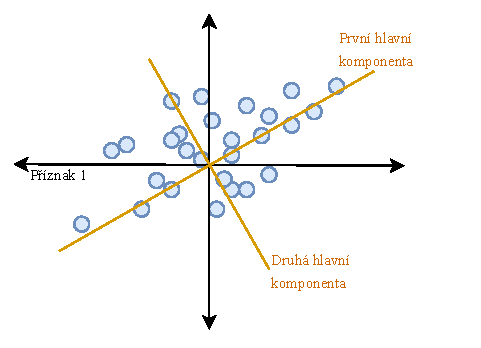
\includegraphics[width=0.7\textwidth]{obrazky/PCA.pdf}
    \caption{Znázornění dvou hlavních komponent na pro dvě proměnné. Zdroj: vlastní.}
    \label{obr:met:PCA1}
\end{figure}

Získání předpisů pro další hlavní komponenty je analogické. Obecně lze zapsat metodu PCA a převod původních proměnných následujícím maticovým zápisem
\begin{equation}
    \mathbf{Y} = \mathbf{XA}, 
\end{equation}
kde $\mathbf{Y}$ obsahuje komponenty $\bm{y}_{1}, \bm{y}_{2}, \ldots$, $\mathbf{X}$ je matice vstupních dat, $\mathbf{A}$ je matice vlastních vektorů kovarianční matice $\mathbf{C}$. Pro matici $\mathbf{A}$ zároveň platí $\mathbf{C} =  \mathbf{A} \mathbf{\Lambda} \mathbf{A}^\top$, kde $\mathbf{\Lambda}$ je diagonální matice vlastních čísel $\mathbf{C}$.\cite{bib:PCA2}

\subsection{Korespondenční analýza}

Vícenásobná korespondenční analýza (anglicky \emph{Multiple correspondence analysis}, dále jako MCA) je metoda, která umožňuje popsat vztahy mezi daty, které jsou popsané kategorickými proměnnými, vytvořením kontingenční tabulky. V~případě, že se popisuje vzájemná relace pouze dvou proměnných, se použije základní korespondenční analýza\footnote{anglicky \emph{correspondence analysis} (CA)}. MCA je alternativou~k PCA, pokud jsou analyzovanými daty kategorická data. \cite{bib:MCA1}

% \subsubsection{Princip korespondenční analýzy}
\subsubsection{Značení}
%https://statmath.wu.ac.at/courses/CAandRelMeth/caipA.pdf
Nechť $\mathbf{N}$ je matice dat s~rozměry $I\times J$, kde I odpovídá počtu pozorování a J je počet kategorií. %asi pocet kategorii, najit !!!
Matice $\mathbf{N}$ je převedena na korespondenční matici $\mathbf{P}$ vydělením matice $\mathbf{N}$ jejím celkovým součtem $n = \sum_{i=1}^{I} \sum_{j=1}^{J} n_{ij}=\mathbf{1}^\top_I \mathbf{N}\mathbf{1}_J$. To zaručuje, že součet prvků matice $\mathbf{P}$ je roven jedné. Tyto kroky lze shrnout následujícím matematickým zápisem
\begin{equation}
    \mathbf{P} = \frac{1}{n}\mathbf{N}, \qquad \mathbf{P} = \{p_{ij}\},  \qquad  \sum_{i=1}^{I} \sum_{j=1}^{J} p_{ij} = 1.
\end{equation}
Součet $i$tého řádku, resp. součet $j$tého sloupce je značen následovně
\begin{align*}
    r_i = \sum_{j=1}^{J} \qquad \mbox{ pro } i=1,\ldots,I, \\
    c_j = \sum_{i=1}^{I} \qquad \mbox{ pro } j=1,\ldots,J.
\end{align*}
Vektor $\bm{r} = \mathbf{P} \mathbf{1}_J $ obsahuje všechny řádkové součty matice $\mathbf{P}$, analogicky vektor $\bm{c} = \mathbf{P}^\top \mathbf{1}_I $ obsahuje všechny sloupcové součty téže matice.

Pro další výpočty zavedeme značení pro diagonální matice, které mají na diagonále  řádkový, resp. sloupcový součet
\begin{equation}
    \mathbf{D}_r = \mbox{diag}(\bm{r}), \quad \mbox{ resp. } \quad \mathbf{D}_c = \mbox{diag}(\bm{c}).
\end{equation}

% Pro připomenutí je vhodné dodat, že součet matice P je jedna

\subsubsection[Výpočetní algoritmus základní korespondeční analýzy]{Výpočetní algoritmus základní korespondeční analýzy \cite{bib:CA1,bib:MCA2}}
Označme $\mathbf{S}  = \{s_{ij}\}$ následující matici
\begin{equation}
    \mathbf{S} := \mathbf{D}_r^{-\frac{1}{2}} (\mathbf{P} - \bm{rc}^\top) \mathbf{D}_c^{-\frac{1}{2}}.
\end{equation}
Po té proveďme singulární rozklad této matice
\begin{equation}
    \mathbf{S} = \mathbf{U}\mathbf{\Delta}\mathbf{V}^\top,
\end{equation}
kde $\mathbf{\Lambda} = \mathbf{\Delta}^2$ je matice vlastních čísel $\lambda_k$ pro $k=1,\ldots,K$, kde $K=min\{I-1,J-1\}$. Potom rozměry matice $\mathbf{U}$, resp. $\mathbf{V}$ jsou $I\times k$, resp.  $J\times k$. Dále platí $\mathbf{U}^\top\mathbf{U}=\mathbf{V}^\top\mathbf{V}=\mathbf{I}$.%https://www.wikiwand.com/en/Correspondence_analysis


% Zatímco u PCA je měřítkem úspěchu míra rozptylu popsaná prvními vybranými hlavními komponentami 
Korespondenční analýza měří míru váženého rozptylu, tzv. inercii pomocí vlastních čísel $\lambda_k$ matice $\mathbf{S}$, $\lambda_k$ se pak nazývají hlavní inercie.
Celková inercie je rovna
\begin{equation}
    I = \sum_{k=1}^{K} \lambda_k = \sum_{i=1}^{I}\sum_{j=1}^{J} s_{ij}^2.
\end{equation}

Hlavní komponenta řádků $\mathbf{F}$ je rovna
\begin{equation}
    \mathbf{F} = \mathbf{D}_r^{-\frac{1}{2}} \mathbf{U}  \mathbf{\Delta}.
\end{equation}
Hlavní komponenta sloupců $\mathbf{G}$ je rovna
\begin{equation}
    \mathbf{G} = \mathbf{D}_c^{-\frac{1}{2}} \mathbf{V}  \mathbf{\Delta}
\end{equation}

\subsubsection*{Výpočetní algoritmus MCA}

Předpokládejme, že původní matice kategorických dat má tvar $N\times Q$, tj. $N$ pozorování a $Q$ proměnných. Matici dat převedeme na indikátorovou matici. Indikátorová matice  $\mathbf{Z} $ je vytvořena tak, že kategorická data jsou rozepsána do pomocných pro-\\měnných. Pokud $q$tá proměnná má $J_q$ typů kategorií, tak příslušná indikátorová matice bude mít $J = \sum_{q=1}^{Q}J_q$ sloupců a $N$. Tzn. počet proměnných byl tímto rozepsáním rozšířen z~počtu původních $Q$ proměnných na $J$ proměnných.
% Klasická MCA má dvě podoby.
První způsob MCA aplikuje základní algoritmus korespondenční analýzy na matici  $\mathbf{Z}$, takto se získají souřadnice pro $N$ pozorování a $J$ kategorií.

% https://towardsdatascience.com/famd-how-to-generalize-pca-to-categorical-and-numerical-data-2ddbeb2b9210 
% https://arrow.tudublin.ie/cgi/viewcontent.cgi?article=1227&context=scschcomdis

% \subsection{Particle Swarm Optimization}

% https://www.analyticsvidhya.com/blog/2021/10/an-introduction-to-particle-swarm-optimization-algorithm/

\section{Korelační analýza}
\label{sec:Teoriekorelace}
\subsection{Korelační koeficient}

Pojem korelace obecně znamená vzájemný vztah mezi dvěma veličinami. Pokud se jedna veličina mění, pak se mění dle míry korelace i druhá veličina. Samotná korelace ale neurčuje míru vztahu, ani směr vztahu. Tedy která veličina je příčinou a která důsledkem. Tuto vlastnost popisuje kauzalita. Míra korelace mezi dvěma veličinami je určena pomocí korelačního koeficientu. Existuje více způsobů měření míry korelace, v~následující části jsou popsány vybrané z~nich.\cite{bib:MB}

Nejčastěji používaným koeficientem pro měření korelace je \emph{Pearsonův korelační koeficient}. Nechť $X$ a $Y$ jsou náhodné veličiny s~realizacemi $x_1, x_2, \ldots$ a $y_1, y_2, \ldots$, potom hodnota Pearsonova koeficientu se vypočítá jako:
\begin{equation}
    r_p = \frac{\mathrm{cov}(X,Y)}{\sigma_X\sigma_Y} = 
    \frac{ \sum_{i=1}^{n}(x_i-\bar{x})(y_i-\bar{y}) }
    {
        \sqrt{
            \sum_{i=1}^{n}(x_i-\bar{x})^2
            \sum_{i=1}^{n}(y_i-\bar{y})^2
            }
    } 
    = \frac{ \sum_{i=1}^{n}x_i y_i - n\bar{x}\bar{y} }
    {
          (n-1) s_{x} s_{y}
    }
\end{equation}
kde $\bar{x}, \bar{y}$ jsou výběrové průměry, $s_x, s_y$ výběrové směrodatné odchylky.\cite{bib:MB}

Tento koeficient měří lineární vztah mezi dvěma proměnnými. Hodnoty se pohybují v~intervalu $\langle -1, 1 \rangle$. Krajní hodnoty znamenají dokonalou lineární závislost. Pokud je koeficient roven 1, pak pokud roste jedna veličina, roste i hodnota druhé veličiny. Pokud je koeficient roven -1, potom s~rostoucí hodnotu jedné veličiny, klesá hodnota druhé. Zatímco je-li hodnota koeficientu rovna nule, veličiny jsou lineárně zcela nekorelované. Pro výpočet totoho koeficientu je předpokládána normalita zkoumaných dat.\cite{bib:MB}

Další koeficient, který měří korelaci mezi dvěma veličinami, je \emph{Spearmanův korelační koeficient}. Tento neparametrický koeficient měří nelineární závislost dvou veličin, určuje, jak moc jejich vztah odpovídá monotónní funkci. Spearmanův koeficient je robustní vůči odlehlým hodnotám a nevyžaduje normalitu dat, protože pracuje se seřazenými hodnotami obou veličin. Hodnoty opět leží mezi $-1$ a $1$ a platí pro mě analogická tvrzení jako Pearsonův korelační koeficient.\cite{bib:MB,bib:correlation}

Nechť $X$ a $Y$ jsou náhodné veličiny s~realizacemi $x_1, x_2, \ldots$ a $y_1, y_2, \ldots$ a číslo $x_{ri}$ je pořadí čísla $x_i$ v~rámci všech hodnot veličiny $X$, číslo $y_{ri}$ je pořadí čísla $y_i$ v~rámci všech hodnot veličiny $Y$. $\bar{x}_r, \bar{y}_r$ jsou průměrná pořadí a $s_{x_r}, s_{y_r}$ příslušné směrodatné odchylky. Vztah pro výpočet Spearmanova koeficientu je:
\begin{equation}
    r_s =
    \frac{ \sum_{i=1}^{n}x_iy_i - n\bar{x}_r\bar{y}_r }
    {
          (n-1) s_{x_r} s_{y_r}
    }.
\end{equation}
Pokud předpokládáme, že pořadí hodnot je unikátní, tj. neexistují v~rámci jedné veličiny hodnoty realizace se stejnou hodnotou, pak lze vzorec pro výpočet Spearmanova korelačního koeficientu zjednodušit na:
\begin{equation}
    r_s = 1-
    \frac{ 6 \sum_{i=1}^{n}d_i^2 }{n(n^2-1)},
\end{equation}
kde $d_i = (x_{ri} - y_{ri})$ je diference pořadí hodnot veličin $X$ a $Y$.\cite{bib:MB,bib:correlation}

Jak je patrné ze vzorců pro oba korelační koeficienty tato míra lze aplikovat pouze na numerické veličiny. V~případě kategorických veličin by bylo potřeba je převést na číselné hodnoty. K~tomu slouží řada metod. Mezi dva nejznámější způsoby překódo-\\vání kategorických proměných patří one-hot kódování a label kódování. V~případě one-hot kódování se ale může počet proměnných výrazně zvýšit, pokud v~datech existují příznaky s~větším počtem unikátních kategorií. Pro druhý zmíněný způsob kódování je nevýhodou fakt, že přiřazením čísel od 0 do $n$, kde $n$ je počet kategorií v~příznaků, se kategorickým hodnotám přiřadí pořadí, které ale v~datech vůbec nemusí být a tudíž je tato nová informace v~datech na obtíž. Další možností je předělat kategorické hodnoty na spojité hodnoty pomocí cílového sloupec (tj. vysvětlované proměnné), tímto způsobem ale může dojít k~zanesení informace o předpovídaném sloupci přímo do vysvětlujících proměnných. \cite{bib:encoding}. Proto jsou v~další části této sekce uvedeny vybrané způsoby měření závislosti dvou kategorických proměnných.

\subsection{Další způsoby měření závislosti}

Pro měření míry závislosti dvou kategorických proměnných lze použít \emph{Cramerovo V}, dále značeno jako $V$. 
Hodnota koeficientu se pohybuje mezi 0 a 1. 1 znamená dokonalou závislost mezi proměnnými, 0 neznamená žádnou závislost. Tento koeficient nemůže nabýt negativní hodnoty, tj. neexistuje negativní závislost. Stejně jako předchozí koeficienty pro korelaci je $V$ symetrické a nezáleží na pořadí veličin.\cite{bib:correl,bib:MB}

Pro dvě zkoumané veličin $X, Y$ s~hodnotami $x_1, x_2, \ldots, x_r$ a $y_1, y_2, \ldots, y_s$ existuje kontingenční tabulka $\mathbf{K}$ těchto veličin, jejíž prvky jsou četnosti hodnot proměnných $n_{ij}$,tj. kdy byly pozorovány hodnoty pro dvojici $(x_i, y_j)$. $r$, resp. $s$ je počet řádků, resp. sloupců kontingenční tabulky $\mathbf{K}$.
Vzorec pro Cramerovo $V$ má tvar:
\begin{equation}
    V~= \sqrt{\frac{\chi^2 / n}{min(r-1, s-1)}},
\end{equation}
kde statistika $\chi^2$ se výpočítá následovně
\begin{equation}
    \chi^2 = \sum_{i=1}^n \frac{(n_ij - n_in_j/n)^2}{n_in_j/n},
\end{equation}
kde $n_i$ je četnost výskytu hodnoty $x_i$, $n_j$ je četnost výskytu hodnoty $y_j$. Tedy platí $n_i=\sum_{i=0}^r{n_{ij}}$ a $n_j=\sum_{j=0}^s{n_{ij}}$.\cite{bib:statology,bib:correl,bib:MB}

Pro určení kolik informace o jedné proměnné nese druhá proměnná, je popsáno
pomocí \emph{ vzájemné informace} \cite{bib:MI}. Informací lze rozumět obsah jakéhokoli oznámení nebo údaje, který se přenáší v~daném čase a prostoru. Podle Shannona, zakladatele teorie informace, je informace míra množství neurčitosti nebo nejistoty o nějakém náhodném jevu, která se odstraní realizací daného jevu \cite{bib:MI2}. Informací tak může být stanovení výsledku náhodného jevu, tedy se jedná o hodnotu náhodné veličiny \cite{bib:MI}. Pro definování vzájemné informace je třeba definovat ještě \emph{vlastní informace} a pojem \emph{entropie}.

Dále jsou sepsány předpoklady pro výpočet množství informace. Pokud má náhodný jev $X$ $n$ realizací, pak je množství informace funkcí $n$. Pakliže je $n=1$, množství informace se rovná nule, neboť se jedná o jev jistý. 
Pokud jevy $X$ A $Y$ probíhají nezávisle, ale ve stejný čas, tj. $p_{XY}(x,y)=p_X(x)\cdot p_Y(y)$, potom množství informace obou jevů se tovná součtu jejich množství.
Pokud jev $X$ má $n $ realizací a jev $Y$ $m$ realizací, kde $m>n$, potom se očekává, že množství informace jevu $Y$ je větší než množství in
formace jevu $X$. \cite{bib:MI2} Pokud je pravděpodobnost každé realizace stejná, tj. $p_X(x) = 1/n$, pak  Hartleyho míra informace je definována jako funkce $I: \mathbf{N} \leftarrow \mathbf{R}$ ve tvaru $I(n)=\log n$. Pro vlastní míru informace obsažené ve výsledku $x$ pak platí: \cite{bib:MI2, bib:MI3}
 \begin{equation}
    I(x)=- \log p_{X}(x).
 \end{equation}

Množství informace celého jevu je popsáno entropií náhodné veličiny. Entropie $H(X)$ náhodné veličiny $X$ s~hodnotami $x_1, x_2, \ldots $ s~pravděpodobnostní funkcí $p(x)$ je rovna: \cite{bib:MI2,bib:literatura}
 \begin{equation}
    H(X) = -\sum_x p_{X}(x) \log p_{X}(x).
 \end{equation}

Nechť je dán vektor $(X,Y)$, kde $X$, resp. $Y$ je náhodná veličina nabývající hodnot $x_1, x_2, \ldots $, resp. $y_1, y_2, \ldots$. Náhodný vektor nabývá hodnot $(x_1, y_1), (x_2, y_2), \ldots $. Sdružená entropie vektoru  $(X,Y)$ má tvar: \cite{bib:MI,bib:MI3}
\begin{equation}
    H(X,Y) = -\sum_{(x,y)} p_{XY}(x,y) \log p_{XY}(x,y).
 \end{equation}
Podmíněná entropie s~předpokladem $p_Y(y)>0$: \cite{bib:MI3}
\begin{equation}
    H(X|Y=y) = -\sum_{(x,y)} p_{X|Y}(x|y) \log p_{X|Y}(x|y),
    \label{eq:podmEntropie}
 \end{equation}
kde podmíněná pravděpodobnost je rovna $p_{X|Y}(x|y) = p_{XY}(x,y) / P_Y(y)$.

Pokles entropie se měří pomocí vzájemné informace, tj. platí věta \cite{bib:MI3}:
\begin{equation}
    I(X;Y) = -H(X,Y)+H(X)+H(Y).
 \end{equation}

Vzájemná informace měří ztrátu informace v~důsledku závislosti $X$ a $Y$. Jinými slovy, kolik informace o jedné proměnné $X$ nese druhá proměnná $Y$. Matematicky je vzájemná informace definována následovně: \cite{bib:MI, bib:MI3, bib:literatura}
\begin{equation}
    I(X;Y) = \sum_{(x,y)} + \log \frac{p_{X\vert Y}(x\vert y)}{p_X(x)}
\end{equation}

Míra, která dovede změřit asymetrickou závislost kategorických proměnných se nazý-//vá \emph{Thielovo U}, které se někdy označuje jako koeficient nejistoty. Pro jeho výpočet se používá podmíněná entropie, viz vztah \ref{eq:podmEntropie}. Thielovo $U$  nabývá hodnot z~intervalu $\langle 0, 1 \rangle$, kde 0 neznamená žádnou závislost a 1 dokonalou závislost. Hodnota není symetrická, tj. $U(X,Y)\neq U(Y,X)$, proto se může používat značení, které určuje směr závislosti -- $U(X,Y) = U(X|Y)$. Vzorec pro výpočet koeficientu $U$ je: \cite{bib:thiel,bib:correl}
\begin{equation}
    U(X,Y) = U(X|Y) = \frac{H(X)-H(X-Y)}{H(X)}.
\end{equation}

\section*{Ostatní použité pojmy}

Při analýze dat lze narazit na problém multikolinearity. \emph{Multikolinearita} je vzájemná lineární závislost vysvětlujících proměnných. Jeli $\mathbf{A}$ matice dat (vysvětlujících pro-\\měnných bez předpovídaného sloupce), pak multikolinearita v~datech existuje, pokud platí rovnice pro alespoň jedno nenulové $c_i$: $c_1\bm{a}_1 + ... + c_k\bm{a}_k$, kde $c_i$ jsou konstanty a $\bm{a}_i$ sloupce matice reprezentující jednotlivé příznaky, $k$ počet sloupců matice, tj. počet příznaků. V~reálných datech stačí, když je daná rovnice přibližně splněna.\cite{bib:MB}

Měřítkem multikolinearity je \emph{rozptylový inflační faktor} (zkratka VIF z~anglického variance inflation factor). Možné hodnoty pro koeficient jsou 1 až libovolné číslo větší než jedna, 1 znamená nezávislost. Nad určitou hodnotu koeficientu, v~literatuře \cite{bib:multi} je uvedeno už číslo větší než 5, je značná multikolinearita již přítomna v~datech. Koeficient má pro $i$-tý sloupec matice $\mathbf{A}$ tvar:
\begin{equation}
    VIF_i = \frac{1}{1-R_i^2},
\end{equation}
kde $R_i^2$ je koeficient determinace $i$-tého sloupce. Ten říká, jak velkou část variability závislé proměnné je možné vysvětlit.\cite{bib:multi}

\section{Metoda GUHA}
\label{sec:Teorie:Guha}

Metoda GUHA je původní česká metoda používaná pro neexplorační analýzu dat.
První článek o této metodě vyšel v~roce 1966. V~současné době je jedním z nejrozsáhlejších implementací metody systém LISp-Miner. Jedná se o software vyvíjený na Fakultě informatiky a statistiky Vysoké školy ekonomické v~Praze, kde se zároveň používá pro výuku a výzkum dobývaní znalostí z~databází \cite{bib:GUHA}. Zároveň je také implementována knihovna \emph{CleverMiner} v~jazyce Python, která disponuje částí funkcionalit softwaru LISp-Miner.

\subsection{Základní princip metody}

Cílem metody GUHA je získat z~pozorovaných dat všechny vztahy, které jsou jsou pravdivé pro množinu objektů, ze které pochází zkoumaná data. Využívají se k~tomu statistické testy hypotéz, které dovolují na základě platnosti určitého tvrzení o vzorku dat přijmout tvrzení o celé množině objektů. Pravdivé tvrzení o celé množině dat se nazývá \emph{teoretické tvrzení}. Tvrzení o vzorku dat se nazývá \emph{observační tvrzení}. Vztah $1:1$ mezi těmito tvrzeními zprostředkovávají statistické testy, znázorněno na obr. \ref*{obr:met:GUHA1}.\cite{bib:GUHA}

\begin{figure}[hbtp!]
    \centering
    \captionsetup{justification=centering}
    
\includegraphics[width=.5\textwidth]{obrazky/GUHA/GUHA1.pdf}
    \caption{Vztah mezi tvrzeními vzorku dat a celých dat v~metodě GUHA. Zdroj: vlastní.}
    \label{obr:met:GUHA1}
\end{figure}

Základní postup GUHA procedury je na obrázku \ref*{obr:met:GUHA2}. Vstupem pro procedury jsou vstupní data a parametry, které definují množinu relevantních tvrzení. Na základě definice jsou vytvořena všechna relevantní observační tvrzení, která jsou verifikována podle dat. Výstupem jsou pak všechna všechna prosté observační tvrzení vycházející ze vstupů. Prosté relevantní  tvrzení je takové tvrzení, které je pravdivé ve vstupních datech a zároveň neplyne již z~uvedeného jiného tvrzení ve výstupu.\cite{bib:GUHA}

\begin{figure}[hbtp!]
    \centering
    \captionsetup{justification=centering}
    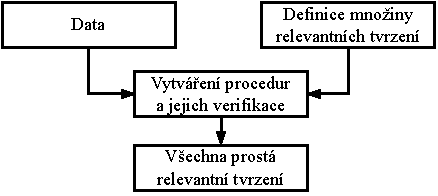
\includegraphics[width=.5\textwidth]{obrazky/GUHA/GUHA2.pdf}
    \caption{Základní postup procedury GUHA. Zdroj: vlastní.}
    \label{obr:met:GUHA2}
\end{figure}

\subsection{Důležité pojmy}


% Uvažujeme potenciálně nekonečnou množinu objektů. Metoda předpokládá výsledky existenci pozorování této množiny reprezentované v~matici dat. Cílem je získat všechny zajímavé vztahy, které jsou pravdové pro celou množinu objektů

Pro podrobnější popis procedur je nejprve třeba definovat několik pojmů, se kterými se v~procedurách pracuje. Metoda pracuje s~násdledujícími pojmy \cite{bib:GUHA}:

\begin{itemize}
    \itemsep0em
    \item \textbf{Matice dat a atributy} -- Řádky matice jsou jednotlivá pozorování. Atributem se rozumí sledovaná vlastnost, jedná se o sloupec matice.
    \item \textbf{Základní booleovský atribut} -- Jedná se o výraz $\bm{\mathrm{A(\alpha)}}$, kde $\bm{\mathrm{A}}$ je atribut a  $\bm{\alpha}$ je vlastní podmnožina $\bm{\mathrm{A}}$. $\bm{\alpha}$ může obsahovat více prvků než jeden.
    \item \textbf{Booleovský atribut} -- Každý základní boolovský atribut je booleovský atribut. Boolovské atributy jsou i negace, konjunkce a disjunkce základních boolovských atributů. 
    \item[] Pro každý řádek $i$ matice $\mathbf{M}$ nabývá boolovský atribut  $\bm{\mathrm{A}}$ hodnotu $0$, nebo $1$.
    \begin{equation*}
    \bm{\mathrm{A}}\left[i\right] = 1 \Rightarrow \mbox{boolovský atribut } \bm{\mathrm{A}} \mbox{ je pravdivý pro řádek } i.
    \end{equation*}
    \begin{equation*}
        \bm{\mathrm{A}}\left[i\right] = 0 \Rightarrow \mbox{boolovský atribut } \bm{\mathrm{A}} \mbox{ je nepravdivý pro řádek } i.
        \end{equation*}

    \item \textbf{Literál} -- Základní boolovský atribut nebo jeho negace.
    \item \textbf{Dílčí cedent} -- Konjunkce nebo disjunkce literálů.
    \item \textbf{Cedent} -- Jedná se o konjunkci dílčích cedentů. Příkladem cedentu je booleovský atribut, který vznikl konjunkcí a disjunkcí dalších atributů.

\end{itemize}


Další pojmy se týkají vztahů, se kterými procedury pracují \cite{bib:GUHA}:

\begin{itemize}
    \itemsep0em
    \item \textbf{Asociační pravidlo} -- Výraz $\mathrm{X} \rightarrow \mathrm{Y}$, kde $\mathrm{X}$ a $\mathrm{Y}$ jsou konjunkce dvojic atribut a jeho hodnota. Dále v~textu je používaná pro tento pojem zkratka AP.
    \item \textbf{Konfidence AP} -- Podíl počtu řádků, které splňují antecedent a zároveň sukcedent a počtu řádků, které splňují pouze sukcedent.
    \item \textbf{Podpora AP} -- Podíl počtu řádků, které splňují antecedent a zároveň sukcedent a počtu řádků vstupní matice dat.
\end{itemize}

Častou úlohou pro dobývání AP je nalezení všech AP, u kterých je hodnota konfidence a podpory AP větší nebo rovna danému prahu. V~rámci GUHA se AP zkoumají jako vztah dvou obecných boolovských atributů, které jsou odvozené ze sloupců vstupní matice. GUHA asociační pravidlo (GUHA AP) je 
výraz 
\begin{equation}
    \varphi \approx \psi, 
\end{equation}
kde $\varphi, \psi$ jsou boolovské atributy, které nemají obsažený žádný společný boolovský atribut. $\varphi$ se nazývá \emph{antecedent} a $\phi$ \emph{sukcedent}\footnote{Antecedent, jako cedent, který předchází a sukcedent, jako cedent, který následuje.}. Symbol $\approx$ odpovídá \emph{4ft-kvantifikátoru}, viz dále v~této sekci. Existují také podmíněná GUHA AP, která mají tvar  $\varphi \approx \psi | \chi$, kde $\chi$ je boolovský atribut.\cite{bib:GUHA}

Pravdivost GUHA AP v~matici dat $\mathbf{M}$ se určuje pomocí tzv. \emph{4ft-tabulky}. Nechť je dána matice vstupních dat $\mathbf{M}$, antecedent $\varphi$, sukcedent $\psi$. Pak \emph{4ft-tabulka} $\mathrm{4ft}(\varphi,\psi,\mathbf{M})$ je definována jako čtveřice čísel $(a,b,c,d)$, pro které platí:
\begin{itemize}
    \itemsep0em
    \item $a$ je počet řádků matice $M$, které splňují oba boolovské atributy $\varphi, \psi$.
    \item $b$ je počet řádků matice $M$, které splňují $\varphi$, ale nesplňují $\psi$.
    \item $c$ je počet řádků matice $M$, které nesplňují $\varphi$, ale splňují $\psi$.
    \item $d$ je počet řádků matice $M$, které nesplňují ani jeden atribut $\varphi, \psi$.\cite{bib:GUHA}
\end{itemize}
Reprezentace této tabulky je zobrazena v~tab. \ref*{tab:GUHA:tabulka}.

\begin{table}[hbtp!]
    \begin{center}
            \captionsetup{justification=centering}
    \caption{\emph{4ft-tabulka} matice $\mathbf{M}$ s~asociačním pravidlem $\varphi \approx \psi$.}
    \begin{tabular}{c|c|c}
        $\mathbf{M}$ & $ \;\psi \;$& $\neg\,\psi$ \\
        \hline
        $\varphi$ & $a$& $b$ \\
        \hline
        $\neg\,\varphi$ & $c$& $d$ \\
        \end{tabular}
    \label{tab:GUHA:tabulka}
\end{center}
\end{table}

\emph{4ft-kvanitifikátor}, symbol $\approx$, definuje podmínku, která se týká hodnot $(a,b,c,d)$ v~\emph{4ft-tabulce}. Kvantifikátor je formálně definovaný pomocí funkce $F_\approx$, která každé čtveřici nezáporných čísel přiřazuje hodnotu $1$, resp. $0$ pokud je, resp. není podmínka splněna. Zapisujeme $F_\approx(a,b,c,d)$ nebo zkráceně $\approx(a,b,c,d)$.\cite{bib:GUHA}
\begin{equation}
\begin{aligned}
    \mbox{GUHA AP } & \varphi \approx \psi \mbox{ je pravdivé v~matici dat }\mathbf{M} \\
    & \Leftrightarrow \approx(a,b,c,d) = 1 \mbox{, formálně zapsáno jako } \mathrm{Val}(\varphi \approx \psi) = 1.   \\
    \vspace*{.5em} \\
    \mbox{GUHA AP } & \varphi \approx \psi \mbox{ je nepravdivé v~matici dat }\mathbf{M} \\
   & \Leftrightarrow \approx(a,b,c,d) = 1 \mbox{, formálně zapsáno jako } \mathrm{Val}(\varphi \approx \psi) = 1. 
\end{aligned}
\end{equation}

Pro podmíněné AP $\varphi \approx \psi | \chi$ platí obdobné vztahy. Předpokládáme však, že boolovský atribut $\chi$ nemá ani jeden společný .atribut s~atributy $\varphi$ a $\psi$. Platí tvrzení \cite{bib:GUHA}:
\begin{equation}
    \begin{aligned}
        &\mbox{Nechť } \mathbf{M} \mbox{ je matice vstupních dat, } \varphi,\psi,\chi  \mbox{ boolovské atributy, } \approx \mbox{ kvantifikátor.} \\
        & \mbox{Podmíněné AP } \varphi \approx \psi | \chi \; \mbox{je pravdivé v~} \mathbf{M} \Leftrightarrow \varphi \approx \psi \; \mbox{ je pravdivé v~matici } \mathbf{M|}\chi.
    \end{aligned}
\end{equation}

\subsection{Procedury}
\label{sec:clever:pojmy}
V dokumentaci \cite{bib:GUHA} je popsáno sedm procedur -- \emph{4ft-Miner,  SD4ft-Miner, CF-Miner, SDCF-Miner,  KL-Miner,  SDKL-Miner,  Ac4ft-Miner} \cite{bib:GUHA}. V~knihovně v~jazyce Python jsou implementované pouze metody \emph{4ft-Miner, SD4ft-Miner, CF-Miner} \cite{bib:GUHAclever}. V~této práci jsem použila metodu pouze první metodu, proto další je další teoretický popis věnován pouze metodě \emph{4ft-Miner}.

Tato procedura pracuje s~AP $\varphi \approx \psi$, nebo s~podmíněnými AP $\varphi \approx \psi | \chi$. V~knihovně \emph{Cleverminer} lze v~hlavní funkci \texttt{cleverminer} předat vstupní DataFrame s~daty, který reprezentuje vstupní matici dat, další parametr je jedna ze tří implementovaných procedur, dále seznam podmínek pro vyhodnocení tvrzení, vypnutí optimalizace, limit pro výsledná tvrzení a seznam cedentů. Cedenty jsou rozděleny na antecedenty (parametr \texttt{ante}, tj. boolovský atribut $\varphi$), sukcedenty (parametr \texttt{succ}, tj. atribut $\psi$) a podmínky (parametr \texttt{cond}, tj. boolovský atribut $\chi$).
Každý z~boolovských atributů libovolného typu cedentu může mít tyto atributy:
\begin{itemize}
    \itemsep0em
    \item \texttt{name} -- Název příznaku matice, tj. název sloupce v~DataFramu.
    \item \texttt{type} -- Jakým pravidlem se řídí výběr více kategorií v~příznaku. Jedna z~hodnot \texttt{subset, lcut, rcut, seq, one}. 
    \item \texttt{minlen} -- Minimální počet kategorií v~daném příznaku.
    \item \texttt{maxlen} -- Maximální počet kategorií v~daném příznaku.\cite{bib:GUHAclever}
\end{itemize}

Příznaky musí být kategorické a musí být možné je seřadit. Druhá vlastnost je třeba pro vybírání více kategorií v~jednom cedentu určitými způsoby selekce. Pro textové řetězce reprezentující kategorie jsou názvy kategorií řazeny podle abecedy.\cite{bib:GUHAclever}

Pro názornost jsou dále uvedeny příklady pro jednotlivé druhy atributu \texttt{type}. Nechť je dán příznak $\mathbf{A}$ s~kategoriemi 1, 2, 3, 4, 5 a parametry jsou definovány následovně: \texttt{minlen=1}, \texttt{minlen=3}. Pokud je typ \texttt{one}, bere se jedna z~kategorií daného příznaku, tuto kategorii je třeba specifikovat. Pro typ \texttt{subset} jsou vybrány všechny následující možnosti:
\begin{itemize}
    \itemsep0em
    \item Délka je rovna 1 --  $\mathbf{A(1), A(2), A(3), A(4), A(5)}.$
    \item Délka je rovna 2 --  $\mathbf{A(1, 2), A(1, 3), A(1, 4), A(1, 5), A(2, 3), A(2, 4), A(2, 5)},$
    \item[] $\mathbf{A(3, 4), A(3, 5), A(4, 5)}.$
    \item Délka je rovna 3 --  $\mathbf{A(1, 2, 3), A(1, 2, 4), A(1, 2, 5),A(2, 3, 4), A(2, 3, 5),}$
    \item[] $\mathbf{A(3, 4, 5)}$.\cite{bib:GUHA}
\end{itemize}
Pro typ sekvence, \texttt{seq} by se pak vybraly následující možnosti:
\begin{itemize}
    \itemsep0em
    \item Délka je rovna 1 --  $\mathbf{A(1), A(2), A(3), A(4), A(5)}.$
    \item Délka je rovna 2 --  $\mathbf{A(1, 2), A(2, 3), A(3, 4), A(4, 5)}.$
    \item Délka je rovna 3 --  $\mathbf{A(1, 2, 3), A(2, 3, 4), A(3, 4, 5)}$.\cite{bib:GUHA}
\end{itemize}

Pro typ \texttt{lcut} se vybírají možnosti:
\begin{itemize}
    \itemsep0em
    \item Délka je rovna 1 --  $\mathbf{A(1)}.$
    \item Délka je rovna 2 --  $\mathbf{A(1, 2)}.$
    \item Délka je rovna 3 --  $\mathbf{A(1, 2, 3)}$.\cite{bib:GUHA}
\end{itemize}
Analogicky pro typ \texttt{rcut}.

Literály v~rámci cedentů lze také kombinovat obdobnými způsoby. Opět lze přiřa-\\dit minimální a maximální délku, typ pro kombinování literálů je výběr konjunkce, nebo disjunkce. Tyto možnosti lze specifikovat pro antecedenty, sukcedenty i pod-\\mínky. Zadání podmínek není nezbytné v~atributech funkce \texttt{cleverminer}.

Další parametry, které lze předat této funkci jsou:
\begin{itemize}
    \itemsep0em
    \item \texttt{Base} (základ) -- Minimální počet řádků, které splňují antecedenty i sukcedenty (číslo $a$ v~tabulce \ref*{tab:GUHA:tabulka}).
    \item \texttt{RelBase} (relativní základ) -- Hodnota základu vydělená celkovým počtem řádků dat (případně počtem řádků v~matici s~aplikovanou podmínkou).
    \item \texttt{conf} (Konfidence) -- Pravděpodobnost $/mathrm{P}(\psi|\varphi)$. Jinými slovy procen--\\tuální zastoupení řádků, které vyhovují $\psi$ (sukcendentům) z~těch řádků, které vyhovují i $\varphi$ (antecendtům).
    \item \texttt{AAD} (nadprůměrná závislost) -- Jak moc $\varphi$ zvyšuje  pravděpodobnost $\psi$. Kolikrát se zvýší pravděpodobnost splnění sukcedentů, když se vezmou pouze záznamy, které vyhovují antecentům, oproti všem záznamům minus 1.
    \item \texttt{BAD} (podprůměrná závislost) -- Jak moc $\varphi$ snižuje  pravděpodobnost $\psi$.
\end{itemize}

Příklad volání funkce \texttt{cleverminer} je sepsaný v~ukázce kódu č. \ref*{code:cleverminer}.
\begin{lstlisting}[language=Python, style=mystyle, label={code:cleverminer}, caption={Příklad volání funkce \texttt{cleverminer}.}]
cleverminer(df = data,
            proc = "4ftMiner", 
            quantifiers = {"conf":0.6, "Base":1000},
            ante = {
                    "attributes":
                    [
                        {
                            "name":"weekday", 
                            "type":"subset", 
                            "minlen":1, "maxlen":3
                        },
                        {
                            "name":"quarter", 
                            "type":"lcut", 
                            "minlen":1, "maxlen":4
                        }
                    ], 
                    "minlen":1, "maxlen":3, "type":"con"
                    },
            succ = {
                    "attributes":
                    [
                        {
                            "name":"L3", 
                            "type":"subset", 
                            "minlen":1, "maxlen":3
                        }
                    ], 
                    "minlen":1, "maxlen":1, "type":"con"
                    },
            cond = {
                    "attributes":
                    [
                        {
                            "name":"promo", 
                            "type":"one", 
                            "value":"promo"
                        }
                    ],
                    "minlen":1, "maxlen":1, "type":"con"
                    }
            )
\end{lstlisting}

\section{Nástroje}



\subsection{Python -- Jupyter Notebook}
Veškeré výpočty probíhaly v~jazyce Python. Metoda GUHA ve verzi Pythonu 3.10, ostatní výpočty a příprava dat ve verzi 3.9. Kód byl napsán a spouštěn v~nástroji\emph{ Jupyter Notebook}. Všechny informace o tomto nástroji jsem čerpala z~dokumentace tohoto nástroje \cite{bib:JN}. Jedná se o alternativu ke konzoli jazyka Python. Jupter Notebooky jsou interaktivní a umožňují psát a spuštět blok po \emph{buňkách}. Buňky jsou sdruženy v~souboru s~příponou \emph{ipynb}, ve skutečnosti se jedná o JSON soubor. V~souboru je uložený kód a zároveň i naposledy spuštěné výstupy jednotlivých buněk. 

Výhodou Jupyter Notebooku oproti klasické konzoli je, že podporuje odsazování, zvýrazňování syntaxe, zobrazení obrázků, HTML prvků nebo \LaTeX výrazů přímo ve výstupu pod kódem. Dále je možné soubor dobře dokumentovat pomocí jazyka Markdown. Tento značkovací jazyk není omezený jen na prostý text, jako jsou klasické komentáře v~kódu. Díky němu lze soubor strukturovat do sekcí různmách úrovní. Vytvořen je tak přehlednější kód. 

Za zmínku také stojí, že dalšími základními programovacími jazyky, které je možné spouštět v~Noteboocích jsou R a Julia. Další jazyky lze spouštět pomocí speciálního jádra pro příslušný jazyk.

S Jupyter Notebooky jsem pracovala v~editoru Visual Studio Code, který podporuje řadu programovacích jazyků. Knihovnu Cleverminer jsem spouštěla v~prostředí Google Colaboratory, které podporuje pouze Jupyter Notebooky.

\subsection*{Databáze}
Data společnosti jsou uložená v~MySQL databázi, ke které jsem přistupovala pomocí nástroje HeidiSQL, což je open-sourcový nástroj pro práci s~databázovými tabulkami. Z~tohoto programu je data možné vyexportovat do formátu CSV. S~exportovanými soubory jsem dále pracovala v~Pythonu.

\subsection{Power BI}
\label{sec:PBI}

Pro vizualizaci dat jsem použila nástroj Power BI Desktop, dále už jen Power BI. Tato aplikace umožňuje vytvořit business intelligence report pro sledovaná data. Data je možné nahrát z~různých datových zdrojů, poté z~nich vytvořit datový model. Na základě tohoto modelu pak lze vytvářet reporty s~nejrůznějšími vizuály. Aplikace má rozsáhlou online dokumentaci, a~to i v~českém jazyce. Veškeré informace o Power BI jsou čerpány z~této dokumentace \cite{bib:PBI}. 

Power BI má tři možná zobrazení -- reporty, data, model. V~reportovací části je možné vytvářet interaktivní vizualizace vstupních dat a sestavit tak i vícestránkový report. Do reportů lze přidávat vizuály pro konkrétní data a míry, upravovat vzhled a vlastnosti vizuálu. Také lze nastovat datové filtry, které se týkají buď konkrétního vizuálu, celé stránky nebo napříč celým reportem. V~sekci data jsou zobrazené všechny řádky aktuálně vybrané tabulky. Uživatel může v~tabulce vyhledávat pomocí filtrů, může přidávat nové sloupce, měnit datové typy sloupců, ale nemůže změnit hdonotu existujících dat v~tabulce. V~sekci model se nachází grafické znázornění datového modelu včetně vztahů mezi jednotlicými tabulkami a jejich sloupci. uživatel může měnit -- odebírat, přidávat, měnit kardinalitu vazeb mezi nimi.

Power BI pro práci s~daty využívá dva jazyky -- jazyk M a jazyk DAX (Data Analysis Expressions). První jmenovaný lze použít při nahrávání dat a jejich zpracování, jazyk se generuje na základě kroků v~GUI aplikace, nebo je možné psát příkazy ve vestavěném editory. Druhý jmenovaný se používá přímo ve vizualizační části pro vytváření nových sloupců a metrik, obsahuje přes 200 předdefinovaných funkcí, které jsou podobné funkcím v~aplikaci Microsoft Excel.

\subsubsection*{Nahrání dat}

Data lze do reportu nahrát tabulková data z~mnkoha typů zdrojů. Je možné se např. připojit přímo k~databázi, získat data z~webu, z~cloudového úložiště, z~textového souboru, souboru z~nástroje Microsoft Excel nebo je také možné spustit Python či R kód, který vytváří data. Nahraná data je možné předzpracovávat v~editoru Power Query, který je součástí Power BI Deskotop. Dále jsou uvedeny příklady úprav v~editoru. Je možné nastavovat záhlaví tabulky, vybírat relevantní řádky a sloupce, přidávat nové sloupce pomocí příkazu v~jazyce M. Tabulku s~daty je možné rozdělit na více tabulek, nebo naopak více tabulek sloučit do jedné, odstranit řádky s~chybějícími hodnotami nebo hodnoty nahradit. V~nástroji lze také vytvářet funkce a proměnné např. pro vygenerování tabulky kalendáře.

Editor zaznamenává provedené změny na datech. Jednotlivé kroky tak lze později případně přeskočit, upravit  nebo lze mezi úpravy vložit nový krok. Posloupnost kroků je ale důležitá, neboť kroky se provádějí postupně. Vložený krok může tedy v~některých případech způsobit chybné vykonání následujících kroků. Na obr. \ref*{obr:PBI:PQ} se nachází ukázka z~editoru Power Query.

Po uložení upravených dat v~editoru se transformovaný model zobrazí v~aplikaci Power BI, kde lze s~daty dále pracovat. Úpravu dat, který model obsahuje lze provádět pouze v~nástroji Power Query. Do editoru lze přistupovat opakovaně i během vytváření reportu, může ale nastat sitace, kdy úprava vstupních dat změní model takovým způsobem, že vizuály přestanou správně fungovat.

\begin{figure}[h!]
    \centering
    \captionsetup{justification=centering}
    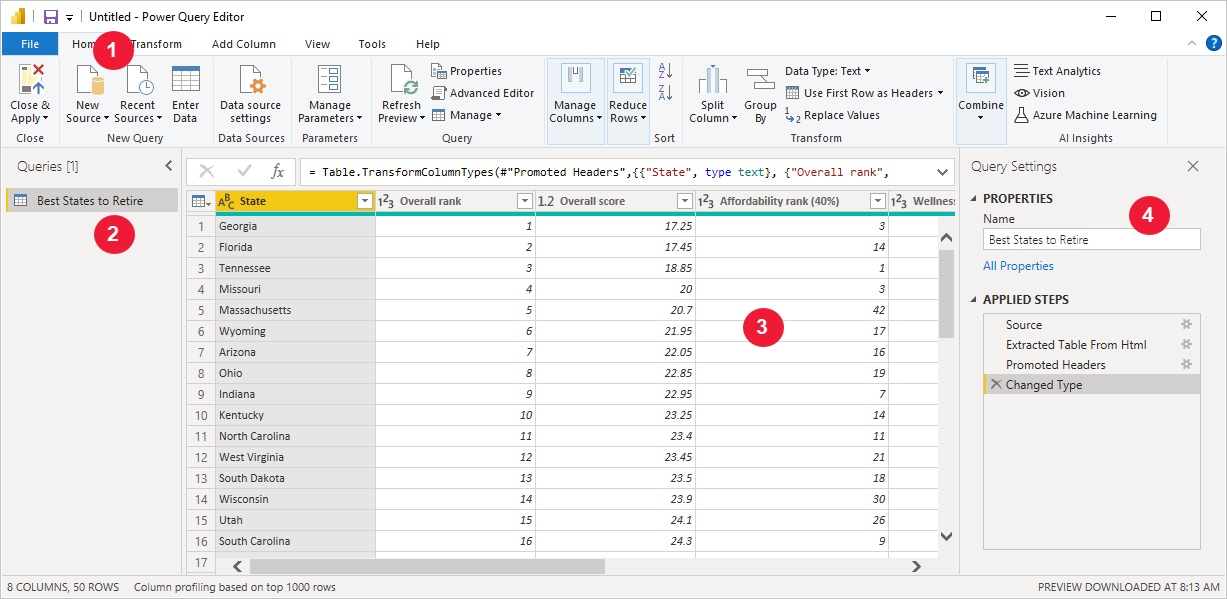
\includegraphics[width=\textwidth]{obrazky/PBIteorie/query-overview-with-data-connection.png}
    \caption{Ukázka nástroje Power Query. \\1 -- Možné interakce s~daty. 2 -- Seznam nahraných tabulek, případně proměných \\a funkcí. 3 -- Ukázka vybraných dat. 4 -- Seznam kroků a vlastností. 
    Zdroj: \cite{bib:PBI}.}
    \label{obr:PBI:PQ}
\end{figure}

\subsubsection*{Míry}

\emph{Míry}, někdy nazývané \emph{metriky} v~Power BI umožňují uživateli reportu sledovat ukazatele, které jsou relevantní pro zkoumaná data. Jedná se o výpočty na datech vytvářené pomocí jazyka DAX. Vypočítaná hodnota míry se mění podle toho, které konkrétní řádky tabulek vstupují do výpočtu, tj. jaké je vizuálu zvolená agregace a vstupní pole. K~přepočítávání dochází automaticky při interakci s~daty v~reportu. Vytvořené metriky jsou zobrazeny vedle seznamu tabulek a sloupců, které se nachází v~datovém modelu. Pro přehlednost jsou ale označeny ikonou. Z~důvodu přehlednosti je ale lepší míry přiřadit do samostatné tabulky, které neobsahuje vstupní data, ale pouze vytvořené míry.

Základní dvě možnosti jak vytvořit metriku jsou -- napsat do řádku vzorců výraz v~jazyce DAX nebo vytvořit tzv. rychlou míru pomocí dialogového okna. Rychlé míry mají ale tu nevýhodu, že nabízí pouze základní operace s~daty jako např. průměr, rozptyl, extrémy, matematické operace nebo převody datumů. 
Při vkládání dat do vizuálu jsou k~dispozici automatické míry, které se neukládají do seznamu měr v~reportu, ale vstupují pouze do vybraného vizuálu. Velmi častou používaná je míra pro počet záznamů, nebo unikátní počet záznamů.

Míru lze buď přímo vložit jako vstup do vizuálu nebo ji použít v~definici jiné míry.

\subsubsection*{Typy vizuálů}

Aplikace nabízí přes dvacet základních vizuálů a stovky vizuálů dostupných ke stažení. V~následující části jsou představeny vybrané vizuály, které jsou použité v~reportu pro data analyzovaná v~této práci. 

Základní graf je graf sloupcový, případně pruhový, které lze dále rozlišit na skládaný, skupoinový a 100\% skládaný graf. Rozdíly mezi těmito grafy jsou na obr. \ref*{obr:PBI:grafy}. Se sloupcovým grafem souvisí i graf kombinovaný, který obsahuje jak sloupce s~hodnotami, tak spojnici pro zobrazení jiných hodnot. Takový graf má tedy dvě rozdílné osy $y$, které mohou mít různá měřítka, ale pouze jednu společnou osu $x$.

\begin{figure}[h!]
    \centering
    \captionsetup{justification=centering}
    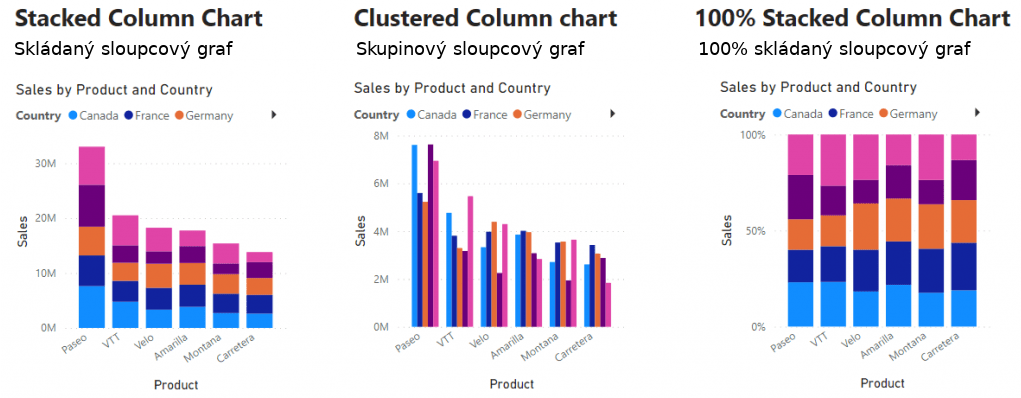
\includegraphics[width=\textwidth]{obrazky/PBIteorie/sloupcove_grafy.png}
    \caption{Základní typy sloupcových grafů. 
    Zdroj: \cite{bib:PBIgrafy}, upraveno.}
    \label{obr:PBI:grafy}
\end{figure}

Další klasický graf je graf bodový, který zobrazuje body v~průsečíku číselných hodnot $x$  a $y$. Osy mohou mít opět různá měřítka. Z bodového grafu vychází tzv. bublinový graf, který ale navíc může zobrazit ještě třetí rozměr v~datech, a to v~podobě velikosti bodů -- bublin. Tvar a poměr velikostí zobrazených bodů, resp. bublin je možné upravovat, stejně tak jejich barvu. Ukázka je na obr. \ref*{obr:PBI:grafybod}.

\begin{figure}[h!]
    \centering
    \captionsetup{justification=centering}
    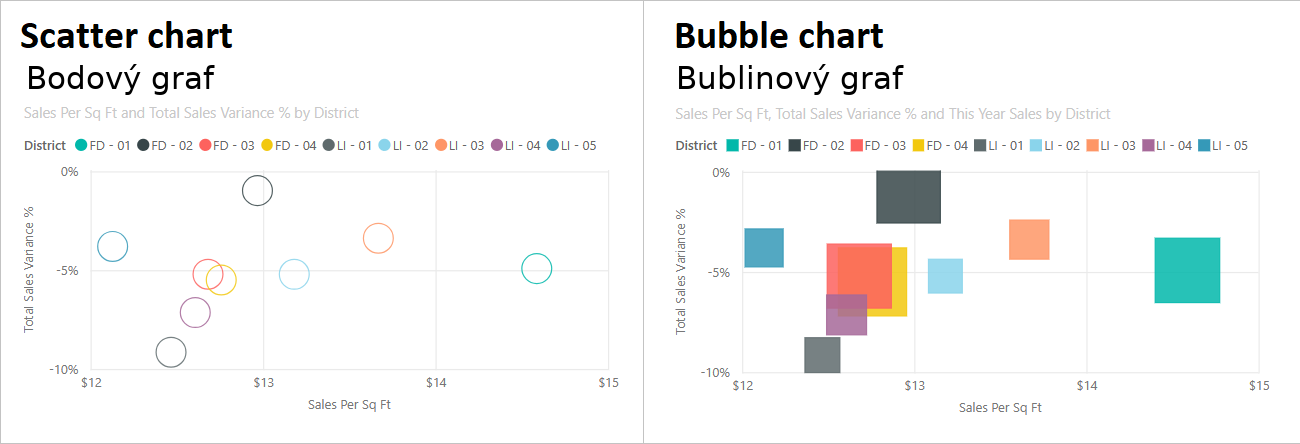
\includegraphics[width=.9\textwidth]{obrazky/PBIteorie/power-bi-compare-charts.png}
    \caption{Základní typy bodových grafů. 
    Zdroj: \cite{bib:PBI}, upraveno.}
    \label{obr:PBI:grafybod}
\end{figure}

Zajímavým vizuálem je mapa stromové struktury. Díky tomuto vizuálu je možné zachytit hierarchická data a poměrové zastoupení kategorií v~datech. Každá kategorie je reprezentována jako obdélník, označuje se pojmem větev. Každý obdélník může obsahovat své podkategorie, označené jako listy. Příklad je na obr. \ref*{obr:PBImapa}.

Formou vizuálu jsou i tabulky, matice a tzv. karty - jednočíselné nebo víceřádkové. Karty se používají pro zobrazení sledované celkové hodnoty, např. celkový počet produktů. Dále karta může obsahovat název sledované hodnoty. Příklad je uveden na obr. \ref*{obr:PBIkarty}. 
Rozdíl mezi tabulkou a maticí je ten, že tabulce lze předávat pouze sloupce a případné číselné hodnoty se spočítají podle agregace v~předchozích sloupcích. Tabulka může obsahovat záhlaví a řádek s~celkovými součty. Matice na rozdíl od obyčejné tabulky umožňuje stupňovité nahlížení na data. Pokud definujeme více vstupních sloupců z~dat jako řádky matice, lze pak záhlaví jednotlivých názvů řádků rozbalit pro větší detail. Příklad tabulky je na obr. \ref*{obr:PBItab.}. 
Příkladem vizuálu jsou i filtry, které lze zobrazit přímo vedle jiných vizuálů a které mohou ovlivnit vizuály na dané stránce. Filtr může být v~podobě dlaždic, seznamu nebo osy v~případě, že se jedná o filtrování časových údajů.

\begin{figure}[hbtp!]
    \centering
    \begin{minipage}{.4\textwidth}
        \centering
        \captionsetup{justification=centering}
        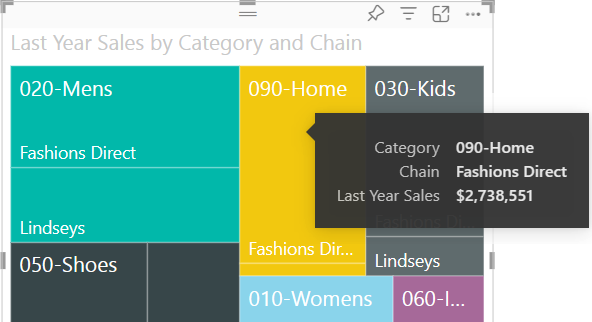
\includegraphics[width=\textwidth]{obrazky/PBIteorie/power-bi-treemap-category-tooltip.png}
        \caption{Mapa stromové struktury s~tooltipem. Zdroj: \cite{bib:PBI}.}
        \label{obr:PBImapa}
    \end{minipage}%
    \hspace*{0.4em}
    \begin{minipage}{.2\textwidth}
        \centering
        \captionsetup{justification=centering}
        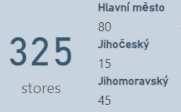
\includegraphics[width=\textwidth]{obrazky/PBIteorie/kartastoresSFF.png}
        \caption{Ukázka vizuálů jednořádková karta (vlevo) a víceřádková karta (vpravo). Zdroj: vlastní.}
        \label{obr:PBIkarty}
    \end{minipage}%
    \hspace*{0.4em}
    \begin{minipage}{.4\textwidth}
        \centering
        \captionsetup{justification=centering}
        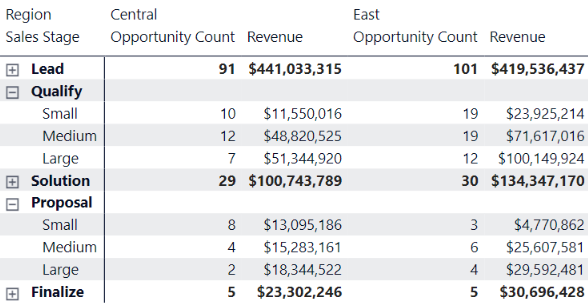
\includegraphics[width=\textwidth]{obrazky/PBIteorie/power-bi-expansion-state.png}
        \caption{Ukázka vizuálu matice. Zdroj: \cite{bib:PBI}.}
        \label{obr:PBItab.}
    \end{minipage}
\end{figure}

\subsubsection*{Vybrané funkcionality}

Ve vizuálech je možnost tooltipu, tedy zobrazení doplňující informace po najetí kurzorem myši na příslušné datové pole, viz obr. \ref*{obr:PBImapa}. Hodnoty, které se zobrazují si uživatel definuje sám. Další velmi výhodnou funkcionalitou Power BI je přechod k~podrobnostem více polí a jednoho pole. První možnost je znázorněna na obr.     \ref*{obr:PBIdrillall}. V~tomto případě se při kliknutí na ikonu $\downdownarrows$ na vizuálu zobrazí data pro další úroveň hierachie. Druhý způsob zobrazí další úroveň hierarchie, která se týká pouze jednoho vybraného pole. Pro zapnutí této volby u vizuálu je třeba zvolit volbu přechodu k~podrobnostem pro jedno pole a poté pole vybrat kurzorem myši. Stejného efektu lze docílit kliknutím pravého tlačítka myši na pole a vybrat příslušnou volbu, tím se přechod rovnou provede. Ikona $\uparrow$ v~obou případech přechází na vyšší hierarchii.

\begin{figure}[h!]
    \centering
    \captionsetup{justification=centering}
    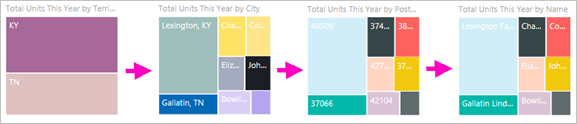
\includegraphics[width=.9\textwidth]{obrazky/PBIteorie/power-bi-drill-path.png}
    \caption{Přechod k~podrobnostem více polí. 
    Zdroj: \cite{bib:PBI}.}
    \label{obr:PBIdrillall}
\end{figure}

Křížové filtrování je další důležitá funkcionalita Power BI. Při kliknutí kurzorem myši na určité pole v~jednom vizuálu se křížově vyfiltrují pole v~ostatních vizuálech na stránce. Jinými slovy jsou odebrána všechna datová pole ve vizuálech, která se netýkají hodnoty ve vybraném poli a dojde k~přepočítání zobrazených měr a ukazatelů. Vedle křížového filtrování existuje ještě křížové zvýraznění. V~takovém případě pole ostatních, nevybraných dat z~vizuálů nezmizí, ale potlačena a vybraná data zvýrazněna. 

Nástroj Power BI disponuje mnoha dalšími funkcionalitami a vizuály, které umožňují analyzovat data a  vytvářet komplexní business intelligence reporty. Přehled všech funkcionalit této aplikace není ale předmětem této práce.

% !!!! TODO:



% \subsection{Genetický algoritmus}

% Genetický algoritmus byl inspirovaný evoluční teorií a přirozeným výběrem. Je založený na teorii, že jedinci, kteří jsou lepší než ostatní mají větší šanci na to, předat svou genetickou informaci dál. Jejich geny tk budou základem nové generace. Podobně jako ve zmíněné teorii, algoritmus používá následující informace: genetickou reprezentaci pomocí bitového  řetězce, funkci pro vyhodnocení tzv. fitness funkci, kombinování genů a mutaci. 

% Nejprve se vytvoří náhodná populace. Od této inicializační populace se postupně se iteruje dokud již další změny nevedou k~lepšímu řešení, nebo dokud neskončí počet iterací. Jedna iterace je analogií k~jedné evoluční generaci.

% Bitový řetězec populace se vyhodnotí pomocí cílové funkce (objective function). Hodnota cílové funkce pak určuje hodnotu fitness daného řešení. Fitness je možné uvažovat jako minimalizační nebo maximalizační kritérium.

% Dále se vyberou dva rodiče podle své fitness hodnoty, kteří se mezi sebou zkříží a jejich potomek vstoupí do další iterace. Jeden ze způsobů výběru je vybrat k~náhodných populací a znich vybrat populaci s~nejvyšším fitness. Křížení rodičů je pravděpodobnostní, takže v~některých případech ,ůže vzniknout potomek stejný jako jeho rodič. Obvykle se hyperparametr pro křížení se nastavuje na vyšší hodnoty např. 80 nebo 90 \%. Dalším parametrem je mutace, ta určuje zda přenesený bit zmutuje nebo ne. Jeho hodnota se nastavuje jako $1/L$, kde $L$ je délka řetězce.





\input{poznamky.tex}

\chapter{Zpracování dat}

Tato kapitola se zabývá popisem práce s konkrétní datovou sadou, kterou jsem obdržela. Z důvodu ochrany dat se v textu nevyskytují přesná pojmenování, ani není možné zobrazit přesnou strukturu uložení dat. 
% TODO, TBD

\section{Popis obdržených dat}

Všechna data poskytnutá společností jsou uložena v databázi, ke které byl zhotoven omezený přístup pro účely získání dat pro analýzy shrinku produktů společnosti. Zároveň s možností přístupu jsem obdržela i tabulku, která stručně komentuje všechny tabulky v databázi a sloupce v jednotlivých tabulkách. Celkem se v databázi nachází přes čtyři sta tabulek, z nichž bylo potřeba vybrat pouze ty, které obsahují relevantní data pro úlohu shrinků.

Z důvodu ochrany dat nelze uvádět přesné názvy tabulek, nicméně pro lepší orientaci v textu, každé použité tabulce přiřadím název, který odpovídá obsaženým datům v tabulce.

\subsubsection{Číselníky}

Základní číselník s údaji o produktech, se nachází v tabulce \texttt{produkt} se 27 sloupci. Pro analýzu vzniku shrinků jsem z této tabulky vybrala jako možné významné údaje následující sloupce:

\begin{itemize}
    \itemsep0em 
    \item \textbf{ID produktu}
    \item \textbf{ID prodejní varianty} -- Určuje o jaký typ balení daného produktu se jedná    
    \item \textbf{Expirace} -- Expirace produktu ve dnech (hodnoty 0, 999 a NULL označují neomezenou expiraci)
    \item \textbf{ID kategorie} -- Kategorie produktu v číselné struktuře (pro lepší interpretaci, o jakou kategorii zboží se jedná, je vhodnější použít strukturu podle úrovní, kterou lze získat napojením na tabulku \texttt{produkt\_kategorie}.)
    \item \textbf{Aktivní} --  Zda je tento produkt stále aktivní v portfoliu, nebo se jedná o produkt, který se již neprodává
\end{itemize}

Tabulka \texttt{produkt\_kategorie} obsahuje převod z číselné struktury do struktury pomocí produktové hierarchie. V obdržených datech má produktová hierarchie šest úrovní. Hierarchie produktů tvoří tedy strom se šesti úrovněmi. Nejvyšší úroveň, tj. úroveň číslo 1 má šest kategorií.

V tabulce \ref*{tab:d:4Bzast} jsou uvedeny počty podkategorií pro každou z kategorií z nejvyšší úrovně. Také je uvedeno procentuální zastoupení kategorií v nejvyšší úrovni v rámci produktového portfolia vybrané společnosti. Zastoupení je odvozeno podle počtu produktů v kategorii.

\begin{table}[hbtp!]
    \captionsetup{justification=centering}
    \begin{center}
    \caption{Počet podkategorií na jednotlivých úrovních a zastoupení \\ nejvyšší kategorie v rámci produktového portfolia.}
    \label{tab:d:4Bzast}
    \begin{tabular}{rp{4cm}  r r r r r  c}
        & Název kategorie & \multicolumn{5}{c}{Počty kategorií} &      Zastoupení kategorie      \\
        \midrule

        Úroveň: & 1       & 2    & 3   & 4   & 5    & 6    &  \\

        \midrule
        & Nepotravinářské    & 1     & 7    & 27   & 76    & 179   & 76,12\%              \\
        & Suché         & 3     & 13   & 33   & 147   & 494   & 7,28\%               \\
        & Kosmetika a drogerie        & 1     & 4    & 21   & 59    & 193   & 7,07\%               \\
        & Čerstvé       & 5     & 11   & 27   & 111   & 469   & 4,27\%               \\
        & Velmi čerstvé & 6     & 10   & 31   & 92    & 271   & 4,04\%               \\
        & Ostatní     & 4     & 4    & 4    & 5     & 5     & 1,06\%               \\
        & Tabák    & 1     & 1    & 1    & 3     & 8     & 0,17\%   \\
    \end{tabular}
    \end{center}
    \end{table}

Poslední, šestá úroveň hierarchie je přímo napojená na hodnotu číselné struktury, která je uvedena v číselníku produktů (v tabulce \texttt{produkt}). Pro získání všech úrovní kategorizace po úrovních k danému produktu je třeba vyhledat v tabulce \texttt{produkt} číselné ID kategorie daného produktu a napojit jej na poslední úroveň v tabulce produktové hierarchie (\texttt{produkt\_kategorie}). V této tabulce je pak uvedena rodičovská kategorie z úrovně 5. Poté je potřeba opět vyhledat v tabulce \texttt{produkt\_kategorie} tuto hodnotu a zjistit její nadřazenou kategorii. Takto se postupuje dokud není dosaženo nejvyšší úrovně. Tyto operace jsem provedla SQL příkazem přímo nad databází. Použila jsem vnitřní spojení na každou úroveň hierarchii na sloupce kategorie a rodičovská kategorie.

Další tabulka, se kterou jsem pracovala obsahuje informace o velikosti a hmotnosti produktů. Tato tabulka je důležitá z toho důvodu, že některé položky jsou vážené. Pokud se udává jejich množství udává se v gramech, zatímco nevážené položky jsou uvedeny v kusech. Aby bylo možné porovnávat oba číselné údaje, ke každému váženému produktu existuje přepočet na počet kusů (ozn. SKU). K tomu jsou využity údaje o počtu kusů na jednu vychystávací jednotku (dále označeno jako $SKU_{\mathrm{VJ}}$) a hmotnost jedné vychystávací jednotky daného produktu (ozn. $m_{\mathrm{VJ}}$). Vychystávací jednotka je jednotka množství používaná pro vychystávání produktů -- jeho balení a transport. Postup pro přepočet hmotnosti produktu na počet kusů ($SKU_{\mathrm{v}}$) je následovný: $$SKU = \frac{m}{m_{\mathrm{VJ}}} \cdot SKU_{\mathrm{VJ}},$$
kde $m$ je hmotnost produktu. Ze vzorce vyplývá, že může vejít neceločíselný počet kusů. Vzhledem k tomu, že tento přepočet se použije k porovnávání velikosti objemů, nikoli k objednávání zboží, tak tato skutečnost není problém.

Číselník prodejen je obsažen v tabulce \texttt{prodejny}. Vybrala jsem z tabulky následující sloupce.
\begin{itemize}
    \itemsep0em 
    \item \textbf{ID prodejny} -- Označení prodejny nebo skladu
    \item \textbf{Název} -- Název prodejny, který obsahuje název města, kde se prodejna nachází.
    \item \textbf{ID kategorie prodejny} -- Do jaké kategorie prodejna nebo sklad patří - zda se jedná o malou nebo velkou prodejnu nebo o sklad.
\end{itemize}

S číselníkem prodejen souvisí číselník pro jejich zařazení do skupin \texttt{prodejny\_skupiny}. Skupiny se mohou v čase měnit. Pro analýzu jsou relevantní tyto sloupce:
\begin{itemize}
    \itemsep0em 
    \item \textbf{ID prodejny} -- Označení prodejny nebo skladu
    \item \textbf{ID skupiny prodejen} -- Prodejny jsou sdruženy do skupin. Ty se například používají pro hromadné objednávání, nebo pro plánování promoakcí.
\end{itemize}    

Promoakce se nachází v tabulce \texttt{promoakce}. Z této tabulky jsou pro následnou analýzu potřebné údaje o ID produktu, počátečním a koncovém datu promoakce a ID skupiny prodejen, na kterých promoakce platí. Promoakce nejsou přiřazené na konkrétní prodejny, ale na skupiny prodejen. Pro další analýzy shrinků je třeba zjistit, zda byl konkrétní zaznamenaný shrink v době záznamu v promoakci, nebo ne. Z tohoto důvodu bylo potřeba tabulky spojit pomocí příkazu \texttt{JOIN} s číselníkem \texttt{prodejny\_skupiny} podle ID prodejny.

\subsubsection{Tabulky transakcí}
V tabulce \texttt{transakce} se nachází údaje o všech provedených transakcích, a to jak skladové transakce, tak prodeje a další pohyby na prodejnách. V případě prodejů prodejen jsou údaje agregované podle prodejny, konkrétního produktu a dne transakce, tzn. v této tabulce nelze rozlišit konkrétní prodeje na jednotlivých pokladnách, ale pouze souhrn za jeden den. Tabulka obsahuje údaje za posledních dvanáct měsíců.

Tabulka transakcí obsahuje 21 sloupců, jako možné podstatné sloupce pro analýzu jsem vybrala následující sloupce:

\begin{itemize}
    \itemsep0em
    \item \textbf{ID transakce} -- Jedinečné pro každou transakci.
    \item \textbf{ID produktu} -- Produkt kterého se transakce týká. Každá transakce obsahuje údaje pouze o jediném produktu. 
    \item \textbf{ID prodejny} -- Transakce je takto přiřazená prodejně, případně skladu. % Z důvodů ochrany dat jsem původní ID převedla na hodnoty od 0 do $p$, kde $p$ je počet prodejen. %TODO TBD (jo chci to tam?)
    \item \textbf{Datum transakce} -- Jedná se o obchodní datum, pokud samotná transakce proběhne až po půlnoci uvedeného dne, tak se posílá s datem z předchozího dne, neboť obchodně patří do toho dne.
    \item \textbf{ID promoce} -- Příznak zda a v jaké promoční akci se produkt nacházel v čase uvedeném v datu transakce. V rámci zpracování dat vyplynulo, že tento příznak není zcela věrohodný 
    \item \textbf{ID shrinku} -- Obsahuje označení jednotlivých typů shrinků viz sekce \ref*{sec:shrinkyTypy}. Celkem je identifikováno sedmnáct typů shrinků. V databázi tento sloupec označuje i jiná ID než ta, která se týkají shrinků, z toho plyne, že bylo třeba vyfiltrovat pouze ta data, která obsahují sedmnáct identifikačních čísel označující shrinky. % Z důvodu anonymity dat jsem původní ID přečíslovala na celočíselné hodnoty od 0 až do počtu shrinků (pro obě hlavní kategorie). %TODO TBD (jo chci to tam?)
    \item \textbf{Objem} -- Množství produktu uvedené v transakci. U kusových produktů se jedná o celočíselný údaj u vážených to je desetinné číslo.
    \item Hodnota transakce v nákladové ceně (desetinné číslo).
    \item Hodnota transakce v prodejní ceně včetně DPH -- v případě prodejů se jedná o skutečnou cenu, u zbylých transakcích je uvedena odpovídající cena podle ceníku.
\end{itemize}

Tabulku, která obsahuje údaje o jednotlivých prodejích na prodejnách společnosti, jsem pro účely této práce nazvala \texttt{transakce\_prodeje}. Celkem obsahuje třináct sloupců. Tato tabulka je vhodná pro analýzu shrinků typu snížení ceny, analýzou tohoto typu se tato práce nezabývá. Pro ostatní typy, není tato tabulka relevantní. Stejně tak není třeba zkoumat ceník jednotlivých produktů, protože v souhrnné tabulce transakcí je již uvedená hodnota transakce v prodejní ceně.

\subsubsection{Další datové zdroje}

Dále jsem pracovala s daty z databáze Českého statistického úřadu \cite{bib:czso}. Na webové stránce úřadu je dostupný odkaz ke stažení souboru ve formátu xlsx. Soubor obsahuje údaje o 237 českých městech za posledních několik desítek let. Některá města obsahují záznamy až sto let nazpět, jiné nemají tak dávno zaznamneanou historii. Dataset obsahuje údaje o lokalite, o počtu obyvatel, o sňatcích, rozvodech, stěhování obyvatel a další. V rámci přípravy dat bylo potřeba napojit prodejny k údajím o okresu, kraji a počtu obyvatel, kteří žijí v okolí prodejny. Soubor s demografickými údaji bylo třeba převést do tabulkové struktury, kde každý řádek patří jednomu městu, protože původní struktura byla nastavená, co list v souboru, to jedno město. Navíc stejné informace nejsou vždy umístěné stejně na každém listu. 


% \subsection{Období jednoho roku}

% 
Sledovala jsem tři různé veličiny, kterými lze hodnotit transakce - počet záznamů (tj. počet řádků) v tabulce \texttt{transakce}, celkové množství produktů a celková nákladová cena produktů. 

Z databáze jsem vybrala všechny transakce za rok 2022, u kterých byl evidován nějaký typ shrinku. Celkem se jednalo o %doplnit!!!
záznamů. Data jsem agregovala po jednotlivých měsících a pro každý měsíc vypočítala pomocí nástroje pivottables.


typ shrinku v závislosti na expiraci
typ shrinku v závislosti hlavní kategorii produktu
typ shrinku v závislosti na dni v měsíci
typ shrinku v závislosti na dni v týdnu

typ shrinku v závislosti na prodejně, neboli typu prodejny nebo v závislosti na centrálním skladu.
Závislost mezi prodejnami a typem produktu


\subsubsection*{Celkový přehled}

Nejprve jsem určila zastoupení jednotlivých shrinků během celého roku, a to bez uvažování závislosti na jiných faktorech. Poměr rozdělení lze vidět na obrázku \ref*{obr:rok:g:celkemD}.
Největší zastoupení, z pohledu všech tří sledovaných charakteristik, má shrink označující prošlé a zkažené zboží. Z pohledu počtu záznamů činí $70{,}24$ \% ze všech shrinků typu damage, což odpovídá 13 milionům řádkům záznamů. V případě množství neprodaných kusů produktů bylo v roce 2022 odepsáno 40 milionů kusů (tj. $65{,}67$  \%). Podle nejdůležitějšího ukazatele - nákladové ceny - tento shrink měl za následek ztrátu 635 milionů Kč (tj. $57{,}94$) \%.
Další damage shrinky, které mají zastoupení větší než 10  \% je shrink označující poškozené zboží a shrink s produkty, které byly odevzdány potravinové bance.
Zbylé shrinky mají v ročním pohledu malý počet výskytů a jejich výskyt bude analyzován v závislosti na dalších faktorech. 

\begin{figure}[hbtp!]
    \centering
    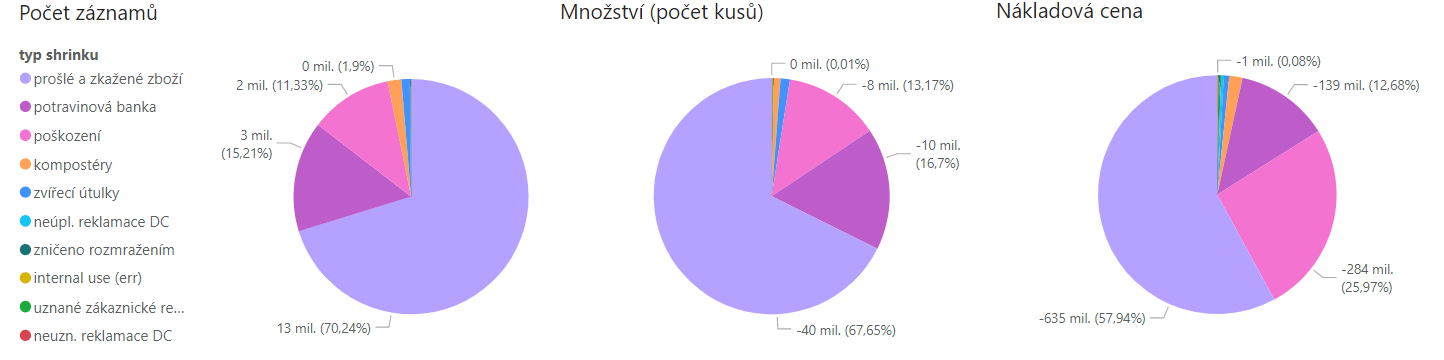
\includegraphics[width=\textwidth]{obrazky/grafy/Graf_celkem-D.png}
    \caption{Zastoupení shrinků typu damage v roce 2022.}
    \label{obr:rok:g:celkemD}
\end{figure}

\subsubsection*{Závislost typu shrinku na čase}

Porovnala jsem množství zaznamenaných shrinků v závislosti na dnech v týdnu, porovnání lze vidět na obr. \ref*{obr:rok:g:tydenD}. Jednotlivé typy jsou zastoupeny analogicky jako v souhrnném přehledu shrinků za jeden rok, tj. prošlé zboží, zboží zaslané do potravinové banky a poškozené zboží. Počty záznamů pro všechny dny jsou v rozmezí $1{,}6$ až $1{,}9$ milionů záznamů  za jeden rok. %!!! nebylo by lepsi tam dat prumer souctu za mesic za cely rok???

\begin{figure}[hbtp!]
    \centering
    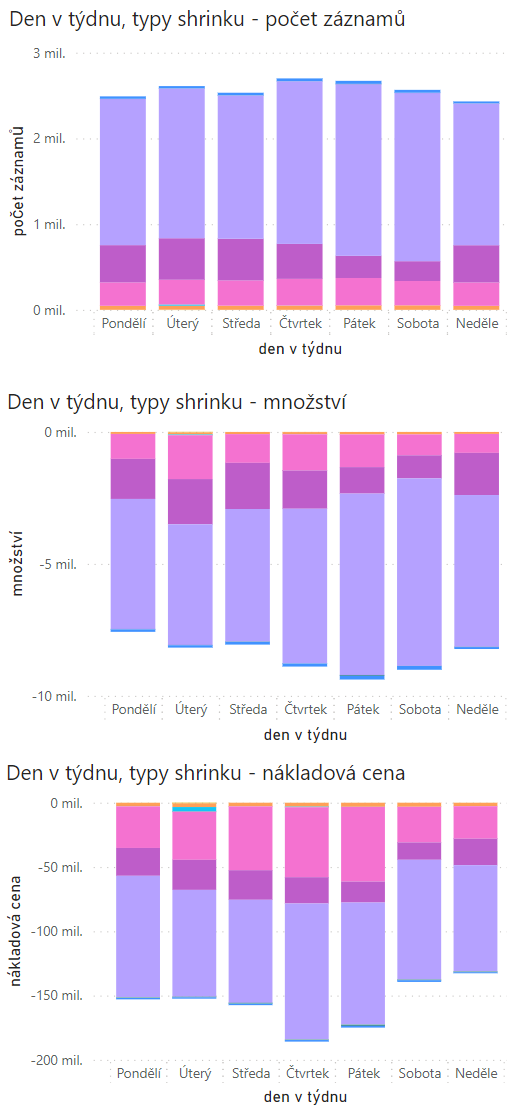
\includegraphics[width=0.5\textwidth]{obrazky/grafy/Grad_dny_tyden-D.png}
    \caption{Zastoupení shrinků typu damage v závislosti na dni v týdnu (údaje pro rok 2022).}
    \label{obr:rok:g:tydenD}
\end{figure}

\begin{figure}[hbtp!]
    \centering
    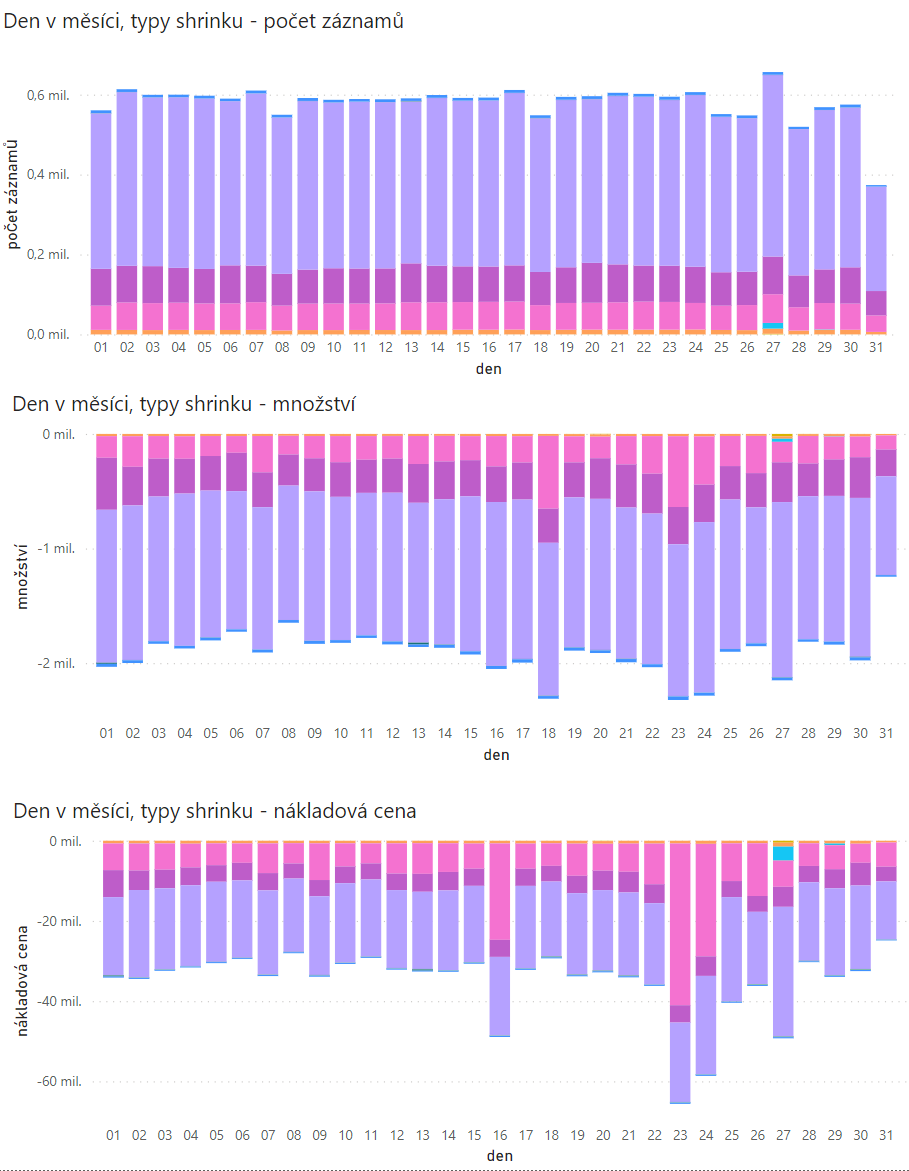
\includegraphics[width=\textwidth]{obrazky/grafy/Grad_dny_mesic-D.png}
    \caption{Zastoupení shrinků typu damage v závislosti na dni v měsíci (údaje pro rok 2022).}
    \label{obr:rok:g:mesicD}
\end{figure}

\subsubsection*{Závislost typu shrinku na hlavní kategorii zboží}

Kategorií, u které bylo evidováno nejvíce damage shrinků je kategorie produktů \emph{superfresh}. V rámci této kategorie je opět nejčastější příčinou odpisu zboží překročená doba expirace, u \emph{superfresh} produktů spíše viditelné zkažení zboží, neboť část \emph{superfresh} produktů nemá uvedenou dobu spotřeby. Druhý nejčastější shrink je shrink označující potravinovou banku. Zbylé shrinky jsou pro tuto kategorii již méně zastoupeny. Kategorie \emph{superfresh} má největší zastoupení většiny typů shrinků nad ostatními kategoriemi - přehled zastoupení jednotlivých shrinků odděleně je na obr. \ref{} %!!! udělat obrazek kde budou vedle sebe grafiký pro kazdy shrink


\subsubsection*{Závislost typu shrinku na typu prodejny}






Vzhledem k vysokému počtu dat pro jeden kalendářní rok, 
v roce 2022 bylo v databázi evidováno přes 32 milionů záznamů o týkající se shrinků
, jsem se rozhodla provést analýzu na měsíčním výběru dat z tohoto období. Jako zkoumaný měsíc jsem vybrala měsíc říjen, neboť v porovnání s letními měsíci a Vánocemi se v říjnu nevyskytují významné sezónní výkyvy.

% [2602933,
%  2439363,
%  2756406,
%  2618723,
%  2809775,
%  2624598,
%  2462898,
%  2545123,
%  2592480,
%  2712669,
%  2543758,
%  2524416]
% 31233142

Zkoumaná říjnová data obsahují $2\ 712\ 669$ řádků a patnáct sloupců. Každý řádek odpovídá jednomu záznamu v databázi shrinku daného produktu. Sledované údaje ve sloupcích jsou: 
% \subsubsection{Sledované údaje}
\begin{itemize}
    \item ID prodejny, kategorická proměnná,
    \item ID produktu, kategorická proměnná,
    \item datum transakce, kategorická proměnná,
    \item typ shrinku, kategorická proměnná,
    \item L1, kategorická proměnná,
    \item L2, kategorická proměnná,
    \item L4, kategorická proměnná,
    \item L5, kategorická proměnná,
    \item L6, kategorická proměnná,
    \item expirace, kategorická proměnná,
    \item množství, spojitá proměnná,
    \item ztracená nákladová cena, spojitá proměnná,
    \item den v týdnu, kategorická proměnná,
    \item číslo den, kategorická proměnná,
    \item období v měsíci (rozdělení měsíce na pět částí), kategorická proměnná.
\end{itemize}
Původní sloupec datum jsem rozdělila na tři jiné proměnné, a to den v týdnu, číslo dne a období v měsíci a sloupec datum jsem vynechala. Z důvodu vysokého počtu záznamů a odlišné povahy dvou typů shrinků jsem data dále rozdělila na shrinky typu damages a shrinky typu inventory. 


\subsection*{Damages shrinky}
Následující část text bude věnována rozboru dat pro shrinky typu damages.



\subsubsection{Výběr dat}
% výběr dle zastoupení shrinků a kategorií produktů a dle outlierů.

Nejprve jsem graficky analyzovala zastoupení shrinků v závislosti na vybraných proměnných pomocí nástroje Power BI, viz obr. \ref*{obr:rok:g:zastoupeni1}. V návaznosti na zjištěné zastoupení shrinků v datech jsem se rozhodla vybrat pouze ty typy shrinků, které tvoří více jak jedno procento z celkových nákladů (tj. náklady činily alespoň jeden milion korun). Vynechala jsem tedy shrinky s označením 5 až 9 a naopak shrinky 0 až 4 byly ponechány. Obdobně jsem přistupovala k záznamům i z hlediska kategorie produktu úrovně L1, jelikož z grafu je patrné, že majoritní zastoupení mají pouze dvě kategorie, a to kategorie superfresh a fresh produktů. Všechny záznamy se zbylými kategoriemi (HBC, others, nonfood, dry food a tobacco) jsem z datasetu odstranila. Těmito kroky jsem zredukovala původní počet řádků datasetu na $1\ 393\ 223$ řádků.

\begin{figure}[hbtp!]
    \centering
    \captionsetup{justification=centering}
    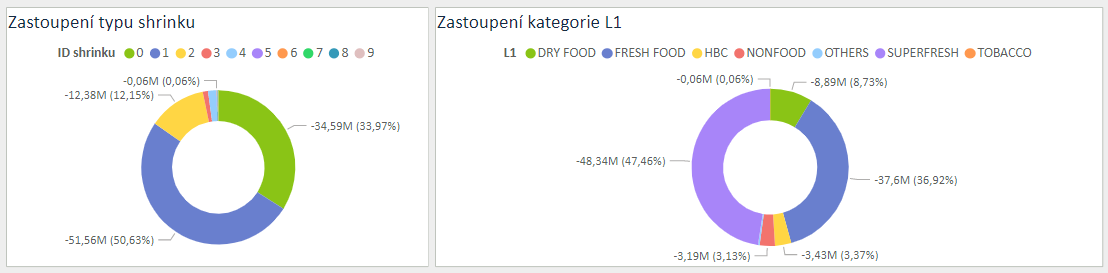
\includegraphics[width=\textwidth]{obrazky/grafy/zastoupeni1.png}
    \caption{Zastoupení shrinků typu damage a zastoupení kategorie L1 v datech \\ z října roku 2022.}
    \label{obr:rok:g:zastoupeni1}
\end{figure}

Jako cílové sloupce (\emph{target} sloupce) jsem určila sloupec s typem shrinku, množstvím produktu a nákladovou cenou. Zbylých jedenáct sloupců slouží jako vysvětlující pro-\linebreak měnné, dále budou označovány jako příznaky pro cílový sloupec. Všechny vybrané příznaky jsou kategorické proměnné, které lze dále rozdělit na nominální a ordinální. Nominální proměnné jsou ID prodejny, ID produktu, kategorie L1, L2, L4, L5 a L6. Ordinální proměnné jsou expirace, den v týdnu, číslo dne a období měsíce. Ordinální příznaky jsem přeznačila tak, aby každá obsahovala pouze hodnoty od nuly do $n_p$, kde $n_p$ je počet kategorií v $p$-tém příznaku. 

Pro další výpočty bylo vhodné přesunout se z nominálních kategorických hodnot na číselné hodnoty. Pro tyto účely jsem zvolila metodu \emph{target encoding}.  %!!! odkaz do teorie, princip meotdy je vysvětlený v kapitole...
Neboť toto kódování na numerické hodnoty zachovává velikost datového souboru, to je klíčové vzhledem k tomu, že nominální proměnné ve zkoumaných datech obsahují velký počet kategorií. Např. počet unikátních produktů v datech je $19\ 026$, což odpovídá stejnému počtu kategorií pro tuto proměnnou. Pokud bych použila one-hot kódování\footnote{One-hot kódování převádí kategorické hodnoty na numerické takovým způsobem že pro každou kategorii vytvoří samostatný sloupec s binárními hodnotami, kde 1 odpovídá dané kategorii a 0 zbylým kategoriím.}  mohlo by dojít k zásadnímu zvýšení počtu sloupců v datech, v tomto případě až o desítky tisíc. \emph{Target kódování} je podobné převodu, který jsem použila pro ordinální proměnné, ale na rozdíl od toho hodnota, která je kategorii přiřazena, souvisí se zastoupením této skupiny v cílovém sloupci a nesouvisí s uspořádáním hodnot uvnitř příznaku. Nevýhodou je, že takto upravená data mohou být náchylná na overfitting, proto je potřeba při predikování použít křížovou validaci.\cite{encoding}

% warehouse_id 339
% product_id 19026
% date_of_transaction 31
% motive_type 10
% cost_value 173409
% L1 7
% L2 20
% L4 141
% L5 450
% L6 1369
% expirace 330
% amount 48634
% weekday 7
% day 31
% quarter_of_month 5

Dále jsem se zabývala identifikací odlehlých hodnot. Nejprve jsem vizualizovala hodnoty pomocí grafu, obrázky \ref*{obr:rok:g:outlierN} a \ref*{obr:rok:g:outlierO}. Z grafu je patrné, že problémová je proměnná $warehouse\_id$, která označuje ID prodejny. Prodejny, které tvoří outliery mohou být malé prodejny, které kvůli menšímu počtu celkových produktů neevidují větší počet shrinků. % !!! jakeho grafu 

\begin{figure}[hbtp!]
    \centering
    \begin{minipage}{.5\textwidth}
        \centering
        \captionsetup{justification=centering}
        
        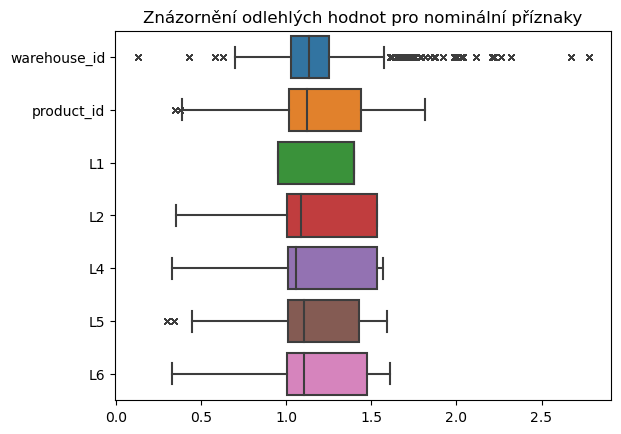
\includegraphics[width=.96\textwidth]{obrazky/zntb/box_nominal.png}
        \caption{Znázornění odlehlých hodnot pro nominální příznaky.}
        \label{obr:rok:g:outlierN}
    \end{minipage}%
    \begin{minipage}{.5\textwidth}
        \centering
        \captionsetup{justification=centering}

        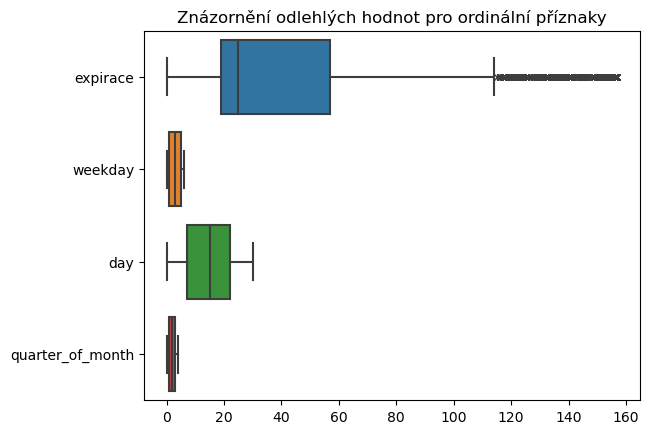
\includegraphics[width=.98\textwidth]{obrazky/zntb/box_ordinal.png}
        \caption{Znázornění odlehlých hodnot pro nominální příznaky.}
        \label{obr:rok:g:outlierO}
    \end{minipage}
\end{figure}

Pomocí Tukeyho testu jsem identifikovala přes $150\ 000$ outlierů pro příznak ID prodejny (\texttt{warehouse\_id}), čímž se dataset zredukoval na $1\ 218\ 453$ řádků. S tímto krokem klesl i počet ostatních outlierů.

V dalším kroku jsem se zaměřila na míru korelace mezi proměnnými. Vizualizovala jsem data pomocí scatter matice pro všechny proměnné, matice je možné vidět na obr. č. \ref*{obr:nb:scatter}. Z této matice můžeme na první pohled vidět, že příznaky odpovídající 4BOX kategorizaci a ID produktu vykazují závislost, což plyne z definice uspořádání této hierarchické kategorizace. V následujících krocích je cílem vybrat tu kategorii, která nejlépe popisuje data ve vztahu k shrinkům.

\begin{figure}[h!]
    \centering
    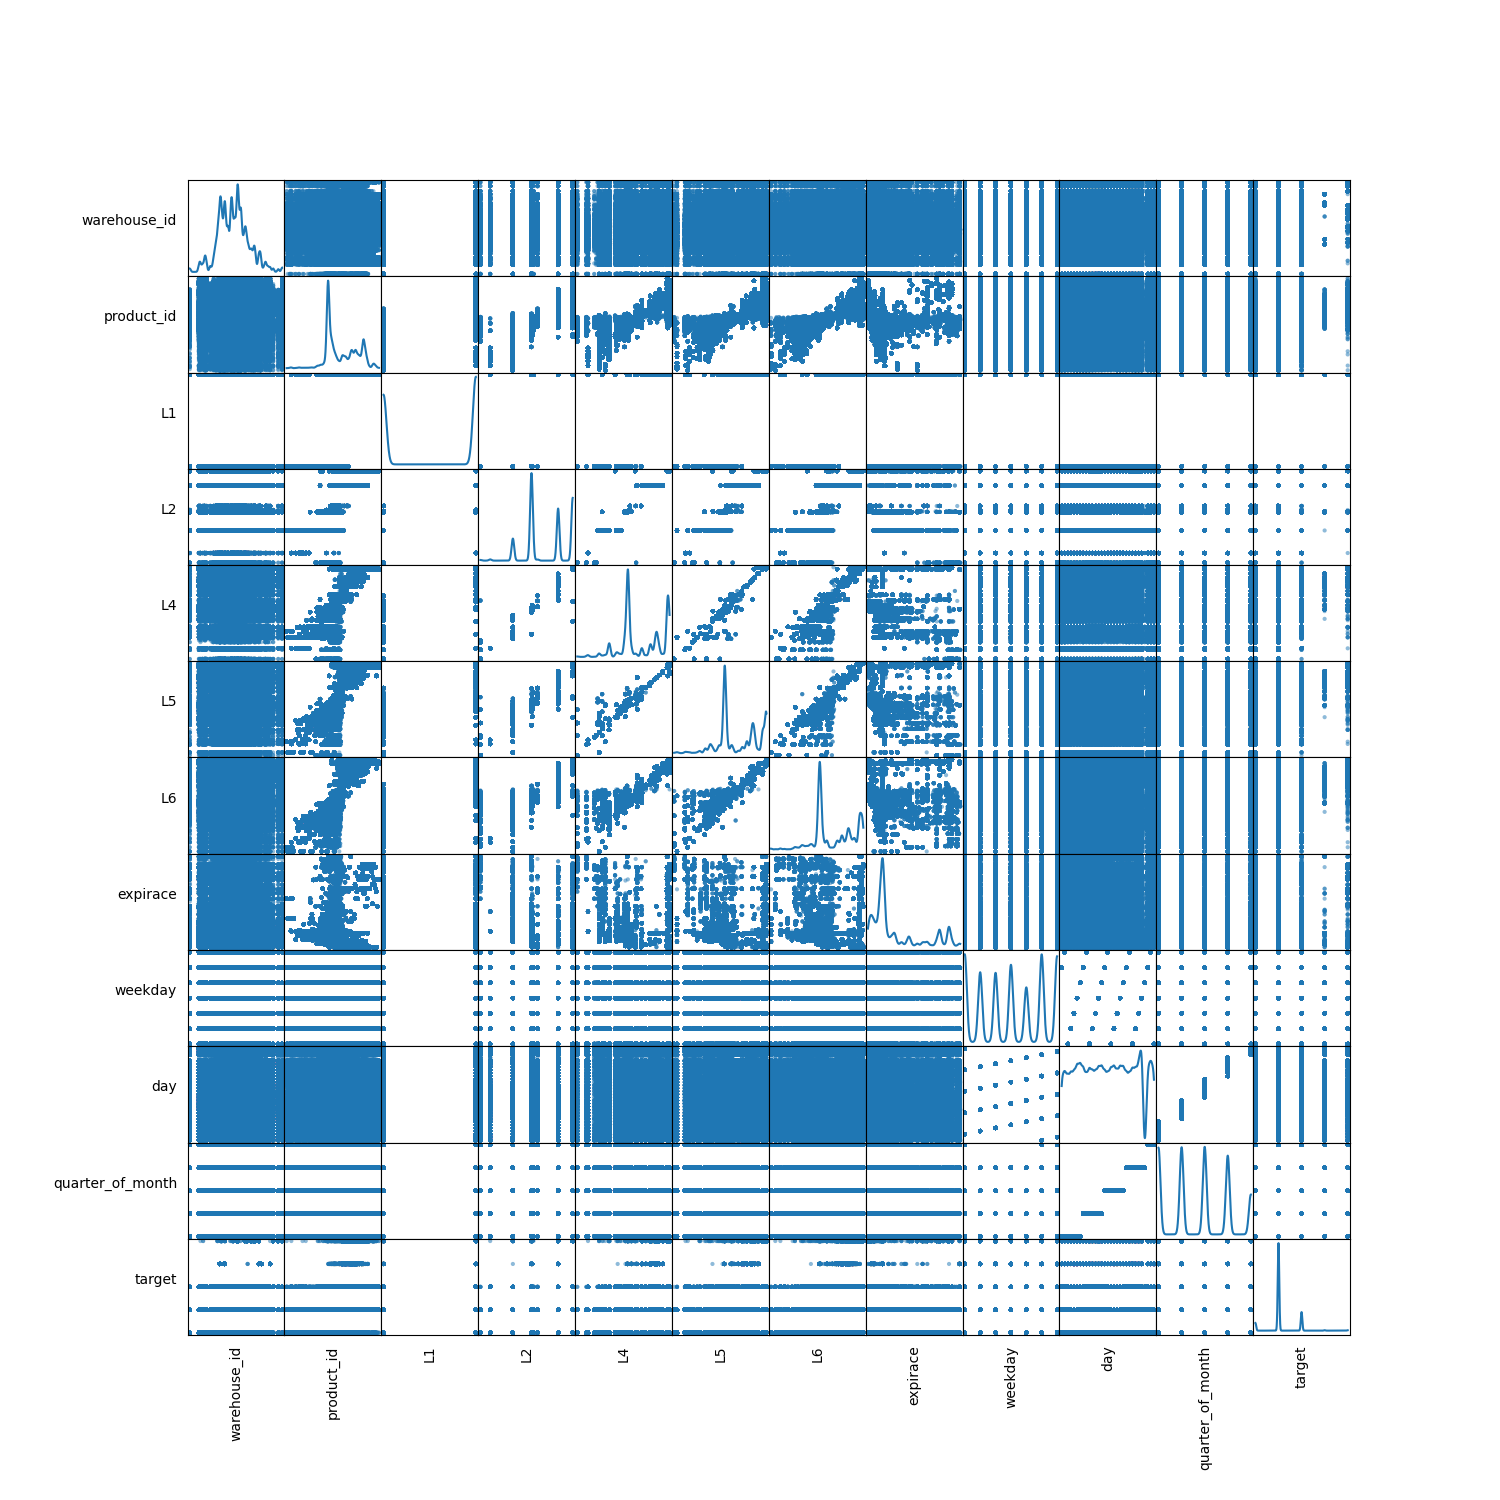
\includegraphics[width=.8\textwidth]{obrazky/zntb/MyScatter.png}
    \caption{Scatter matice příznaků.}
    \label{obr:nb:scatter}
\end{figure}
 
Jako první metodu jsem zvolila $\chi^2$ test. Vzhledem k vysokému počtu dat je matice příliš řídká, a proto nejsou výsledné hodnoty vypovídající a test je tedy pro tuto úlohu nespolehlivý.
Jiným měřítkem pro korelaci mezi proměnnými je Pearsonův korelační koeficient. %!!! odkaz na teorii
Výslednou matici popisující korelační vztahy mezi příznaky jsem vizualizovala teplotní mapou, která je zobrazena na obrázku \ref*{obr:nb:pearson}. Z výsledků je opět patrné, že mezi jednotlivými kategoriemi produktů a produkty je silná korelace. Toto zjištění je zcela logické, neboť se jedná o stromovou strukturu kategorií. Zároveň existuje korelace mezi produktovými kategoriemi a expirací produktu. p-hodnota odpovídající jednotlivým koeficientům byla vždy nulová, kromě pro koeficient týkající se dvojice proměnných expirace a ID prodejny a expirace a pořadí dne v týdnu. Je tedy možné považovat výsledky (kromě těchto dvou výjimek) za statisticky významné.

\begin{figure}[hbtp!]
    \centering
    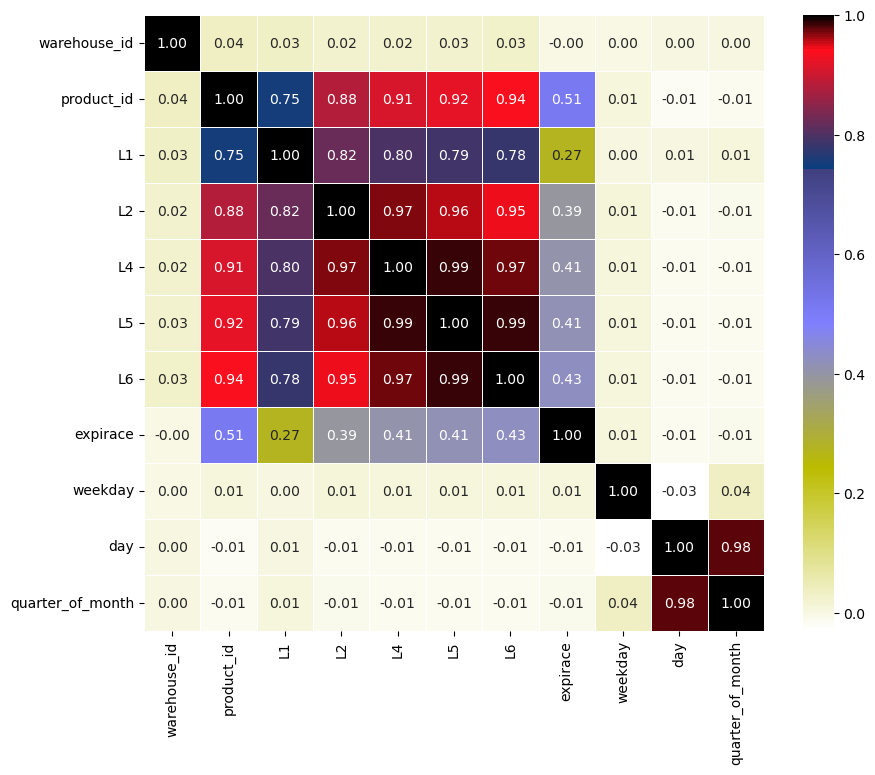
\includegraphics[width=.8\textwidth]{obrazky/zntb/pearson.png}
    \caption{Matice korelačních koeficientů mezi příznaky.}
    \label{obr:nb:pearson}
\end{figure}

Dále jsem použila výpočet koeficientů vzájemné informace \footnote{\emph{mutual information}}, který říká, jaká je podobnost mezi dvěma proměnnými \cite{bib:scikit}. % !!! odkaz na teorii
Matice vypočítaných koeficientů je na obr.\ref*{obr:nb:MI}, jelikož se jedná o symetrickou vlastnost, jsou vynechány hodnoty pod vedlejší diagonálou. Z výsledků je opět vidět zřejmé, že ID produktu sdílí úrovněmi kategorizace tím více, čím je kategorizace jemnější.

\begin{figure}[hbtp!]
    \centering
    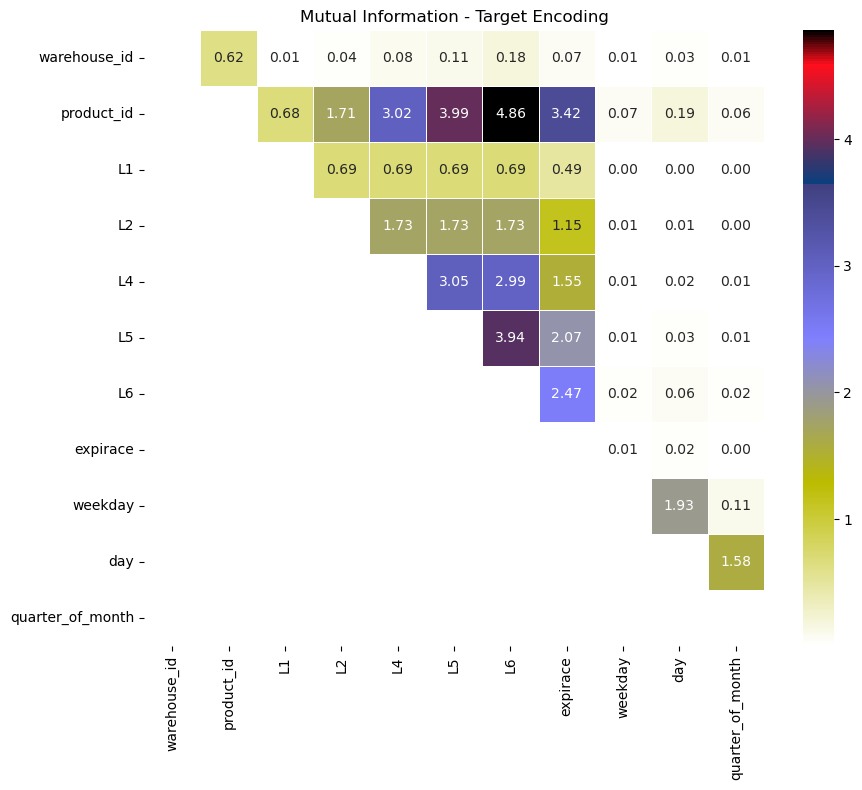
\includegraphics[width=.8\textwidth]{obrazky/zntb/MI_TE.png}
    \caption{Matice koeficientů vzájemné informace mezi příznaky.}
    \label{obr:nb:MI}
\end{figure}

%https://www.statology.org/interpret-cramers-v/
Dále jsem pro znázornění vztahu mezi proměnnými použila koeficient Cramerovo V. Koeficient jsem postupně počítala pro každou dvojici příznaků. Koeficient nabývá hodnot mezi 0 a 1. Číslo blízké nule indikuje, že mezi proměnnými není asociace, číslo blízké jedničce vysokou závislost \cite{bib:statology}. Na obr. \ref*{obr:nb:cramers} lze vidět, že pro kategorie L1 až L6 je hodnota koeficientu  po zaokrouhlení rovna jedné. Vysoká závislost je pak i mezi příznakem expirace a ID produktu a kategorií L1. Dále logicky mezi číslem dne a dnem v týdnu a obdobím v měsíci.
%!!! dopsat co to je %!!!zdroj, odkaz na teorii
\begin{figure}[hbtp!]
    \centering
    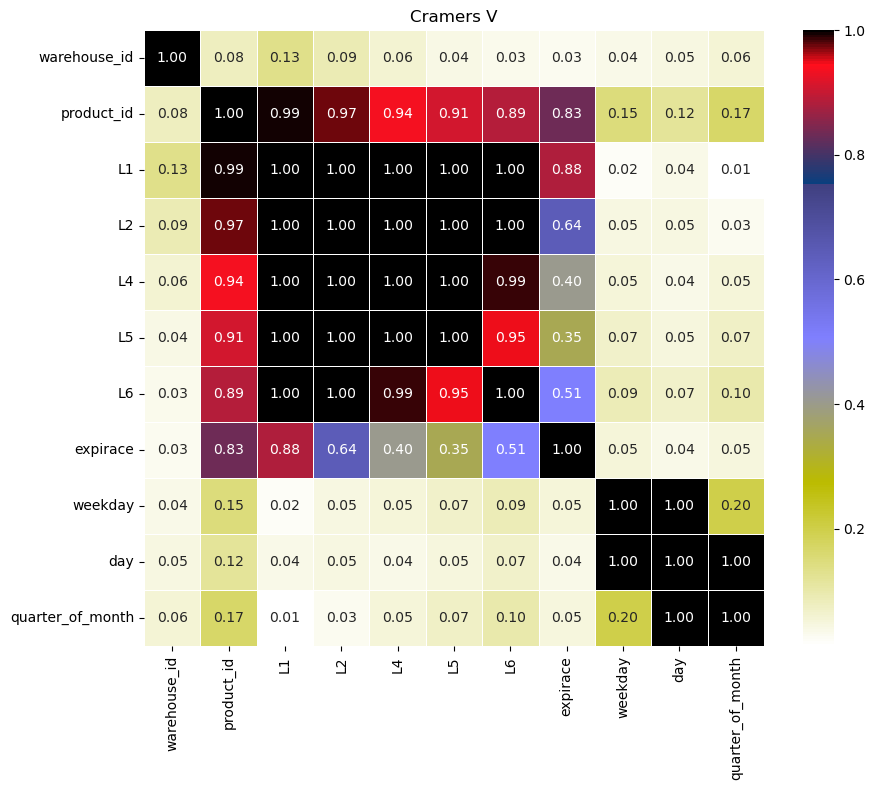
\includegraphics[width=.8\textwidth]{obrazky/zntb/cramers_u.png}
    \caption{Matice koeficientů Cramerovo V mezi příznaky.}
    \label{obr:nb:cramers}
\end{figure}

Další statistikou spočtenou na datech je Theilovo U (neboli koeficient nejistoty), který opět nabývá hodnot mezi 0 a 1 a měří vztah mezi dvěma proměnnými. Na rozdíl od předchozích statistik tento koeficient není symetrický a z výsledků lze vyvodit, ze které proměnné ze dvou zkoumaných můžeme vyvodit informaci o druhé proměnné \cite{bib:correl}. Z výsledků zobrazených v matici na obr. \ref*{obr:nb:thiels} plyne, že z ID produktu lze vyvodit část informace o kategoriích a expiraci. Zatímco úrovně L1 a L2 o ID produktu mnoho informace nenesou. Jak bylo ukázáno i v předchozích statistikách a jak vyplývá z logiky pro získání dne v týdnu a období měsíce, číslo dne nese informaci o těchto dvou příznacích.


\begin{figure}[hbtp!]
    \centering
    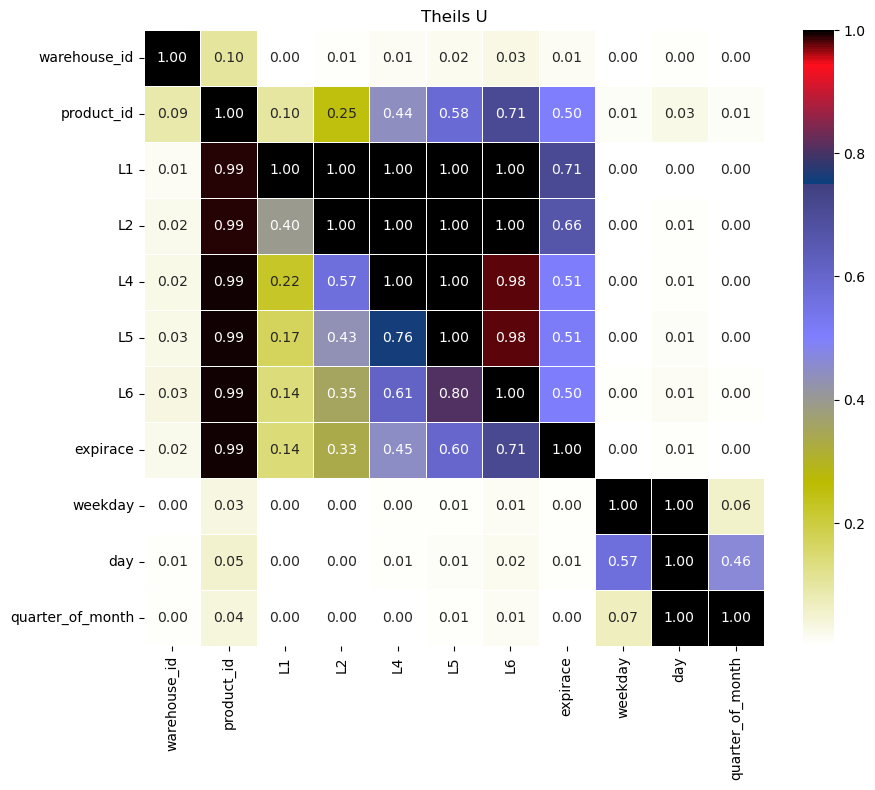
\includegraphics[width=.8\textwidth]{obrazky/zntb/theils_u.png}
    \caption{Matice koeficientů Theilovo U mezi příznaky.}
    \label{obr:nb:thiels}
\end{figure}

Z vypočítaných statistik na datasetu je patrné, že některé příznaky jsou významně závislé, a proto je třeba je z dat odstranit. Kandidáti na vynechání jsou kategorie L2, L4, L6 a číslo dne. V dalších testech budou také vybráni kandidáti a v závěru vyhodnotím, které příznaky byly podle aplikovaných metod vybrány jako vhodné k vynechání a které nikoli.

V dalším testu jsem otestovala multikolinearitu dat pomocí rozptylového inflačního faktoru (VIF). Jako hraniční faktor jsem zvolila hodnotu 40 VIF. Vysvětlující proměnné jsem odebírala z datasetu postupně a odebírání jsem ukončila až, když hodnota VIF nebyla nižší než hraniční.
Tímto došlo k redukci příznaků z jedenácti na pět, a to na kategorii L1, číslo dne, období měsíce, ID prodejny a den v týdnu. Hodnoty koeficientu VIF na datech jsou na obr. \ref*{obr:nb:vif}. 

\begin{figure}[h!]
    \centering
    \begin{minipage}{.5\textwidth}
      \centering
      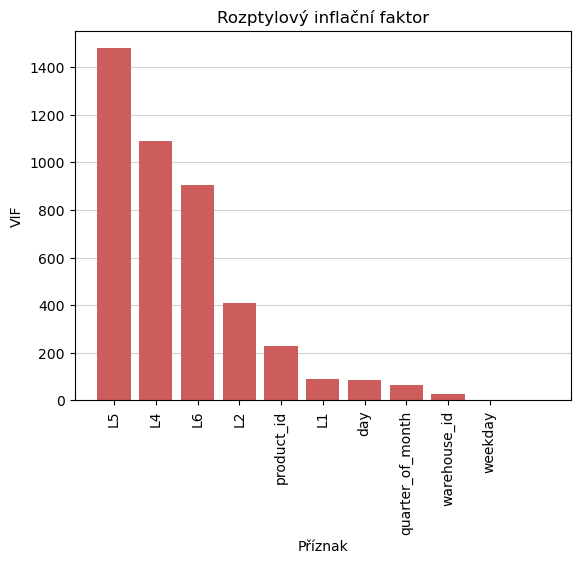
\includegraphics[width=.8\textwidth]{obrazky/zntb/VIF.png}
      \caption{Rozptylový inflační faktor.}
      \label{obr:nb:vif}
    \end{minipage}%
    \begin{minipage}{.5\textwidth}
      \centering
      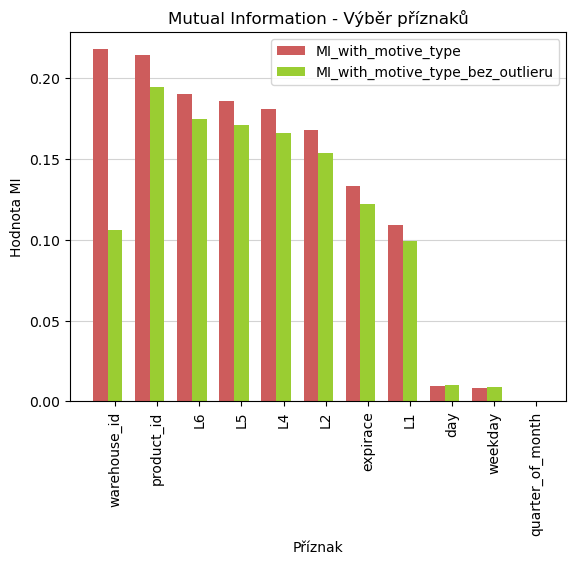
\includegraphics[width=.8\textwidth]{obrazky/zntb/MI_feature_selection.png}
      \caption{Koeficienty vzájemné informace mezi příznaky a cílovým sloupcem typ shrinku.}
      \label{obr:nb:MI_FS}
    \end{minipage}
    \end{figure}

Jako další metodu po výběr příznaků jsem vypočítala hodnotu koeficientů vzájemné informace mezi všemi příznaky s cílovým sloupcem - ID shrinku. Na obrázku \ref*{obr:nb:MI_FS} lze vidět, jak jednotlivé proměnné souvisí s cílovým sloupcem. Pro výpočet tohoto koeficientu jsem použila jak data bez outlierů, tak tenotkrát data před jejich odstraněním. Zde můžeme vidět, že významnost příznaku ID prodejny klesla o téměř polovinu. Nejvíce informace je sdíleno s ID produktu, kategorií L6, dále L5, L4, L2 a expirace. Příznaky související s časovými údaji podle tohoto kritéria nenesou mnoho společné informace.

Jako hlavní metodu pro výběr proměnných jsem se rozhodla použít metodu PCA, tuto metodu je možné použít protože kategorické proměnné jsem převedla na číselné hodnoty v předchozích krocích. Alternativou by bylo použití metody MCA, která se používá pro kategorické datasety, viz dále.
Ve své práci jsem využila implementaci PCA v knihovně \emph{Prince} v jazyce Python. 
Předtím než jsem metodu aplikovala jsem otestovala předpoklad homoskedasticity, tedy shodnost rozptylů v datech, pomocí Bartlettova testu implementovaného v knihovně \emph{factor\_analyzer}. Nulová hypotéza o shodnosti rozptylů nebyla vyvrácena (p-hodnota vyšla nulová). Metodu PCA je proto možné použít.

Na obrázcích \ref*{obr:nb:pca_roztyl_komponetn} a \ref*{obr:nb:pca_kum_roztyl_komponetn} je znázorněno prvních deset komponent a rozptyl který v datech vysvětlují. Na základě hodnot jsem vybrala prvních pět komponent. Již pátá komponenta (označená č. 4) spolu s předchozími vysvětluje více jak 95 \% variability dat. V dalším kroku jsem vypočítala příspěvky příznaků k těmto pěti komponentám a vybrala jsem ty příznaky, které přispívají nejvíce k prvním pěti komponentám. Jejich příspěvek je znázorněný na obr. \ref*{obr:nb:pca_prispevek}. Na základě výsledků analýzy hlavních komponent byly vybrány jako vhodné příznaky pro další práci s daty příznaky - příznaky ID prodejny, den v týdnu, expirace, den a období v měsíci.

\begin{figure}[h!]
    \centering
    \begin{minipage}{.5\textwidth}
      \centering
      \captionsetup{justification=centering}

      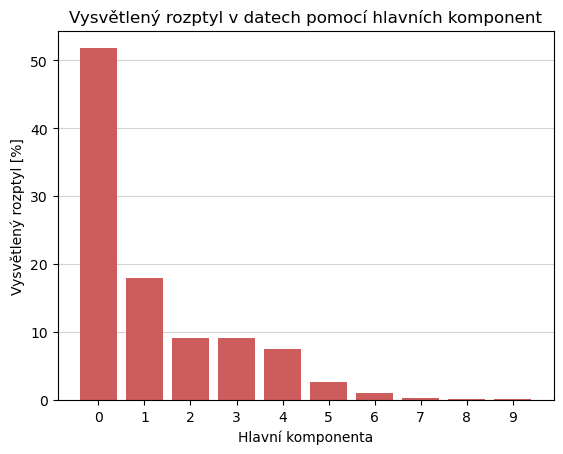
\includegraphics[width=.8\textwidth]{obrazky/zntb/pca-roztyl_komponetn.png}
      \caption{PCA - vysvětlený \\ rozptyl hlavních komponent.}
      \label{obr:nb:pca_roztyl_komponetn}
    \end{minipage}%
    \begin{minipage}{.5\textwidth}
      \centering
      \captionsetup{justification=centering}

      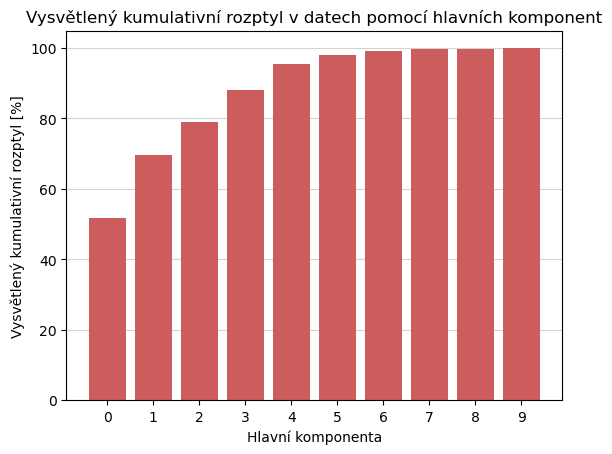
\includegraphics[width=.8\textwidth]{obrazky/zntb/pca-kum_roztyl_komponetn.png}
      \caption{PCA - kumulativní vysvětlený rozptyl hlavních komponent.}
      \label{obr:nb:pca_kum_roztyl_komponetn}
    \end{minipage}
    \end{figure}

\begin{figure}[hbtp!]
    \centering
    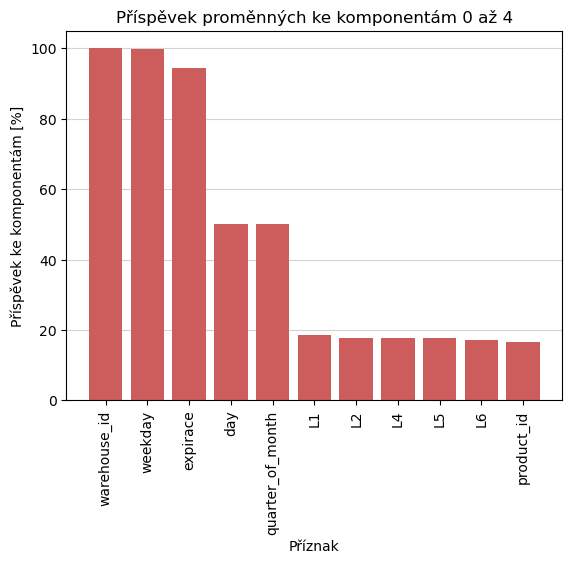
\includegraphics[width=.8\textwidth]{obrazky/zntb/pca-prispevky.png}
    \caption{Příspěvek proměnných ke komponentám 0 až 4.}
    \label{obr:nb:pca_prispevek}
\end{figure}
    
Jak již bylo zmíněno pro redukci dimenzionality u kategorických dat lze použít metodu MCA, opět jsem využila implementaci z knihovny \emph{Prince}. V této implementaci jsou nominální kategorické hodnoty kódovány tak, že narůstá počet sloupců, a proto bylo nutné, vzhledem k nárokům na paměť k uložení matice, omezit množství dat. Vybrala jsem náhodný 20\% vzorek dat, na které jsem MCA aplikovala. Vypočítala jsem prvních pět komponent, které dohromady popisují 79 \% variability dat. Jelikož byla každá kategorie chápána jako samostatná proměnná příspěvky jednotlivých příznaků ke komponentám byly rozmístěny mezi všechny kategorie, nikoli k jednotlivým příznakům. Po agregaci podle původních příznaků největší příspěvek mělo ID produktu, kategorie L6, L5, L4, zatímco nejmenší ID prodejny, L1, den v týdnu a období měsíce. Tyto výsledky je třeba brát se zvážením neboť výpočty probíhali na řádově menším vzorku než u předchozích metod.

% warehouse_id        0.024256
% product_id          1.147270
% L1                  0.035793
% L2                  0.355452
% L4                  0.841652
% L5                  0.911692
% L6                  0.930902
% expirace            0.306007
% weekday             0.035521
% day                 0.362474
% quarter_of_month    0.048981



\chapter{Vizualizace dat}
\label{ch:vizualizace}

Očištěná data vybrané společnosti obsahující záznamy shrinků, které byly způsobeny škodami, jsem vizualizovala v~nástroji Power BI, který se používá pro business intelligence analýzu. Vytvořila jsem report, který umožňuje pomocí interaktivních grafů analyzovat data. První část této kapitoly se věnuje technickému popisu reportu, zatímco druhá část shrnuje výsledky analýzy plynoucí z~reportu.

\section{Popis řešení}
\label{sec:vizualizace:popis}

Report obsahuje pět stránek. První stránka nabízí základní přehled, dashboard, týkající se všech shrinků. Druhá stránka je věnována prodejnám a údajům o lokalitách.
Další stránky se již věnují pouze shrinkům zaviněných škodami a kategoriím Velmi čerstvé a Čerstvé z~produktové hierarchie úrovně 1. Třetí stránka zobrazuje hodnoty ukazatelů hodnoty shrinku a odvozených podílů. Na čtvrté a páté stránce jsou další přehledy z~pohledu konkrétních produktů, kategorií a typů promoakce. Poslední stránka týkající se reportingu je z~pohledu vybraného konkrétního produktu.

Do Power BI souboru jsem pomocí integrovaného nástroje PowerQuery nahrála upravená data z~databáze vybrané společnosti. Hlavní faktickou tabulkou je tabulka \emph{damages}, která obsahuje všechny zaznamenané shrinky z~kategorie shrinků, které byly způsobeny škodami. Druhá faktická tabulka má název \emph{revenue} a obsahuje tržby v~pozorovaném měsíci pro všechny prodejny, tržby jsou dále rozdělené podle kategorie z~úrovně 1 a do čtvrtin měsíce. Doménové tabulky jsou číselník produktů, číselník shrinků a číselník prodejen, dále také číselníkové tabulky, které spojují faktické tabulky -- čtvrtina měsíce a seznam kategorií úrovně 1. 

Datový model tabulek, které jsou vstupem do reportu je znázorněný na obrázku \ref{obr:datmod}. Mezi jednotlivými tabulkami jsou znázorněny vazby -- jejich mohutnost a směr. Tabulka \emph{metrics}, která není navázaná na žádnou jinou tabulku obsahuje výpočetní metriky, které vychází z~dat v~modelu, metriky se dále používají ve vizualizacích.

\begin{figure}[hbtp!]
    \centering
    \captionsetup{justification=centering}
    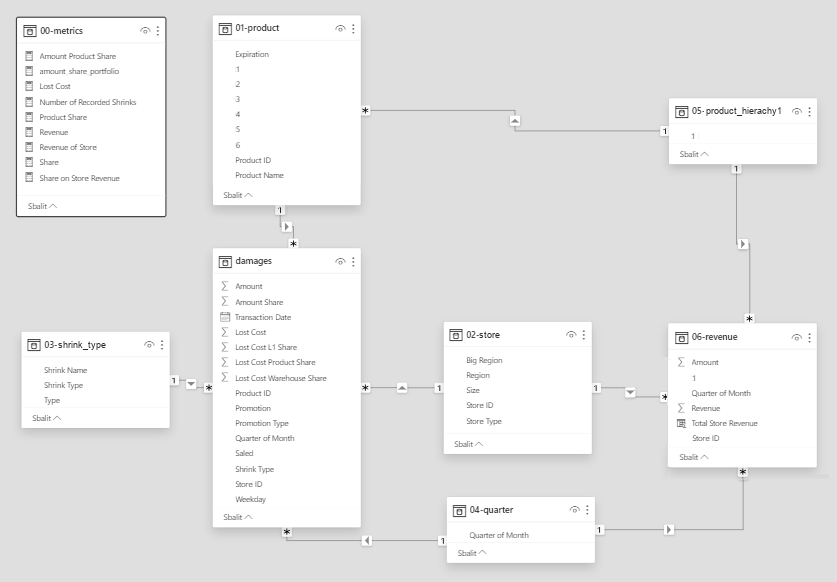
\includegraphics[width=\textwidth]{obrazky/PBI/datmodel.png}
    \caption{Datový model tabulek v~Power BI reportu.}
    \label{obr:datmod}
\end{figure}

Reporting je zpracován v~angličtině, takže i dříve popsané názvy kategorií nebo shrinků jsou přeložené. Překlad je uvedený v~příloze práce. Uvedené tržby v~reportingu odpovídají nekonkrétní peněžní jednotce -- z~důvodu ochrany dat vybrané společnosti byla skutečná čísla vynásobena jistým koeficientem. Poměry zobrazené v~reportu ale vstupním datům společnosti odpovídají.

\subsection{Metriky}

Power BI nabízí uživatelům reportu širokou interakci s~vizuály. Díky metrikám se zobrazené hodnoty přepočítávají podle aktuálních filtrů nebo podle vybraných dat. 

\begin{itemize}
    \itemsep-0.3em
    \item     \textbf{Lost Cost} -- Základní metrika s~hodnotou shrinku ze vstupních dat.
    \item     \textbf{Product Share} -- Základní metrika, obsahuje podíl shrinku na tržbách produktu (přímo ze vstupních dat). Pokud je ve vizuálu agregovaná např. na kategorii nebo prodejnu, vypočítá se její průměr.
    \item     \textbf{Share} -- Základní metrika, obsahuje podíl shrinku na tržbách produktu. Pokud je ve vizuálu agregovaná na prodejnu jedná se celkový evidovaný shrink prodejny dělený tržbou dané prodejny. Pokud je agregovaný podle typu shrinku jedná se o podíl součtu hodnot všech záznamů daného typu a tržeb všech prodejen. Bude-li agregace probíhat zároveň na typu shrinku a na kategorii z~úrovně 1, pak je podíl spočítaný vzhledem k této kategorii typu shrinku zároveň. 
    \item     \textbf{Share on Store Revenue} -- Základní metrika, obsahuje podíl shrinku na celkových tržbách produktu. Tj. pokud je agregace např. podle prodejny a podle kategorie jedná se o podíl všech shrinků produktu z~dané kategorie vydělený celkovými tržbami vybrané prodejny. (Zatímco v~předchozí metrice by se jednalo o tržby pouze za vybranou kategorii.)
    \item     \textbf{Revenue of Stores} -- Celková tržba prodejny za celé sledované období
    \item     \textbf{Revenue} -- Základní metrika s~hodnotou tržeb prodejny rozdělená podle části měsíce podle kategorií z~úrovně 1 a  ze vstupních dat.
    \item     \textbf{Number of Recorded Shrinks} -- Počet záznamů shrinků.
\end{itemize}

\subsection{Reporting}

\subsubsection*{Přehled}

První stránka obsahuje přehled týkající se všech typů shrinků v~rámci kategorie shrinky způsobené škodami, přehled je v~tabulce \ref*{tab:sh:dam} v~kapitole \ref*{ch:shrinky}. Na obr.~\ref*{obr:PBI:overview} je snímek této stránky, pro lepší orientaci při popisu jsem na snímek přidala označující čísla. Na této stránce jsou vyfiltrované všechny kategorie, shrinky i prodejny. V~levé části jsou uvedeny souhrnné informace pro vyfiltrované záznamy (tj. implicitně nic vyfiltrováno není, jedná se o celkové hodnoty) (č. 1). 

Na grafu označeném č. 2, je znázorněno jak velký podíl shrinku na tržbách mají jednotlivé kategorie. Zároveň je barevně označeno, jakou měrou je hodnota zastoupená na malých či velkých prodejnách. Defaultní nastavení vizuálu je zobrazení kategorií úrovně 1, díky funkcionalitě nástroje Power BI je možné postoupit v~hierarchii kategorií níže viz \ref*{obr:PBI:drill}. První graf zobrazuje defaultní pohled, na druhém je vidět výsledek pokud uživatel klikne na ikonu $\downdownarrows$ \emph{přechod k podrobnostem všech polí}. V~takovém případě se postoupí na další úroveň hierarchie napříč všemi kategoriemi. Třetí graf ukazuje stav, kterého uživatel docílí, pokud zaklikne ikonu $\downarrow$ \emph{přechod k podrobnostem jednoho pole}\footnote{Anglicky se přechod k podrobnostem jednoho pole v~nástroji Power BI označuje jako \emph{drill down}.}. V~takovém případě, poté co uživatel klikne na jednu z~kategorií v~grafu (její název nebo příslušný datový pruh), se zobrazí nižší úroveň hierarchie, ale pouze takové kategorie, které jsou podkategorií vybrané kategorie. 
Další graf (č. 3) ukazuje jaký je podíl shrinku na tržbách pro malé a velké prodejny. V~tomto vizuálu po zvolení přechodu k podrobnostem se rozbalí hodnoty podílu pro jednotlivé typy shrinků. Opět jako v~předchozím případě lze postupovat buď pouze pro jeden typ prodejen nebo oba.
Pokud uživatel nezvolí \emph{přechod k podrobnostem jednoho pole} ve vizuálu, ale klikne na datový element ve vizuálu, všechny vizuály na stránkau se křížově vyfiltrují nebo křížově zvýrazní. Rozdíl mezi těmito dvěma akcemi je v~sekci \ref*{sec:PBI}. 
\begin{figure}[h!]
    \centering
    \captionsetup{justification=centering}
    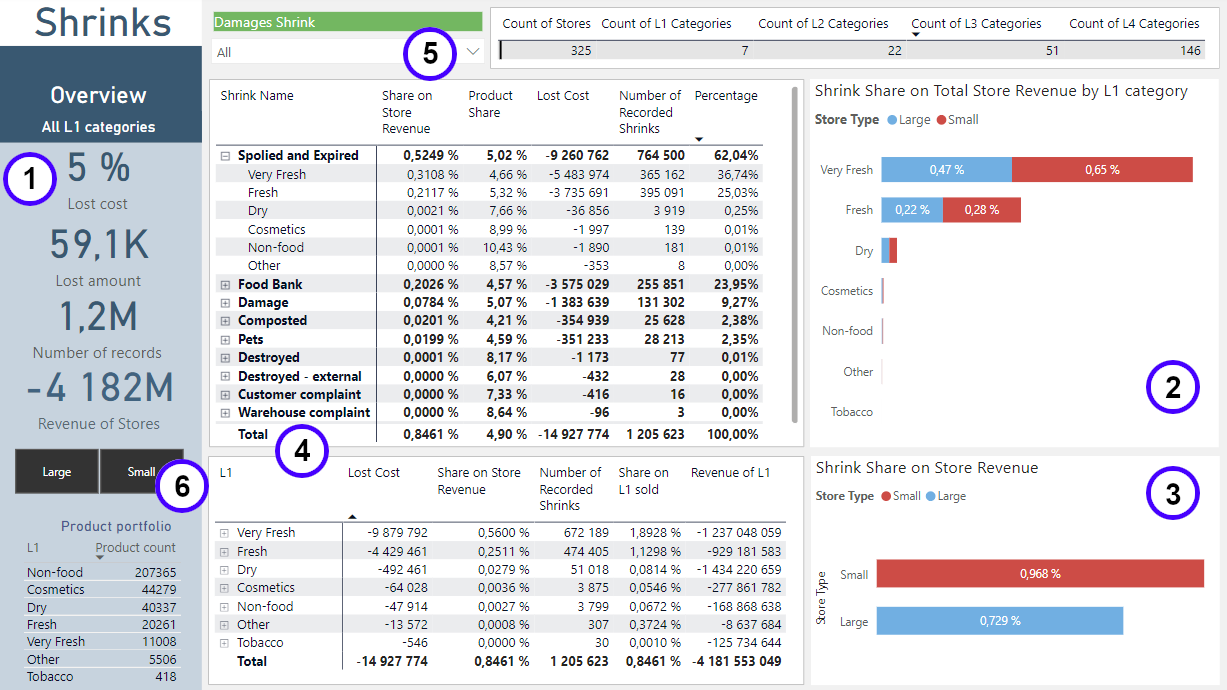
\includegraphics[width=\textwidth]{obrazky/PBI/overview.png}
    \caption{Power BI reporting pro zobrazení údajů o shrincích.}
    \label{obr:PBI:overview}
\end{figure}

Přehledová stránka dále obsahuje dvě tabulky. První tabulka sleduje vybrané ukazatele pro typy shrinků, které lze dále prozkoumat z~pohledu kategorií první úrovně. Druhá tabulka zobrazuje ukazatele z~pohledu kategorií, a to od nejvyšší úrovně po nejnižší, případně až na detail samotných produktů a jejich ID. Vzhledem k tomu, že tabulka může při detailním procházení zabírat více místa je možné přejít na její detail, který se zobrazí přes celou aktuální stránku. Ukázka této tabulky je na obr.~\ref*{obr:PBI:tab1}.
U čísel 5 a 6 jsou umístěny filtry -- pro typ prodejny a pro typ shrinku. Vyfiltrováním příslušného typu se hodnoty v~reportingu automaticky upraví. Všechny nevybrané kategorie nejsou zahrnuté do vizuálů, ani výpočtů hodnot. Např. pokud uživatel vybere pouze velké prodejny, celkové tržby se týkají již pouze všech velkých prodejen, nejde o celkové tržby všech prodejen z~datasetu.

\begin{figure}[h!]
    \centering
    \captionsetup{justification=centering}
    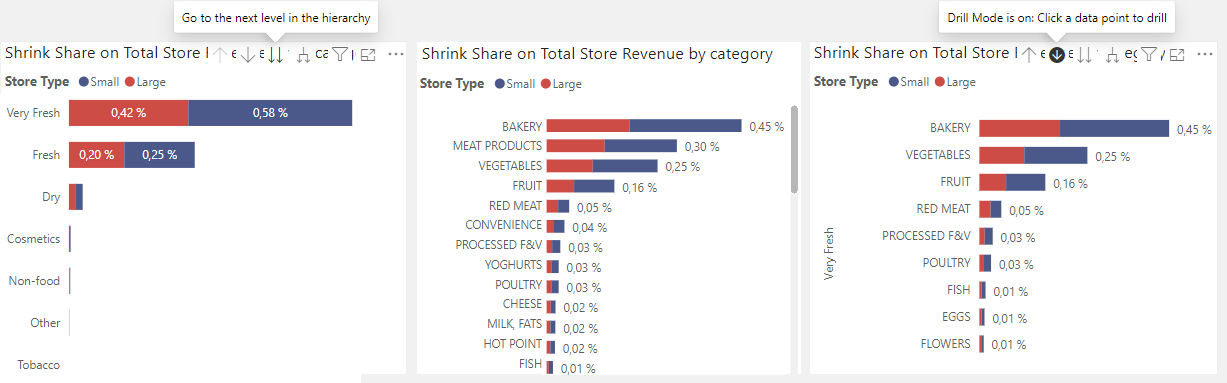
\includegraphics[width=\textwidth]{obrazky/PBI/Catdrilldown.png}
    \caption{Ukázka interakce grafu záznamů shrinku pro přístupy \\ k různým úrovním produktové hierarchie.}
    \label{obr:PBI:drill}
\end{figure}

\begin{figure}[h!]
    \centering
    \captionsetup{justification=centering}
    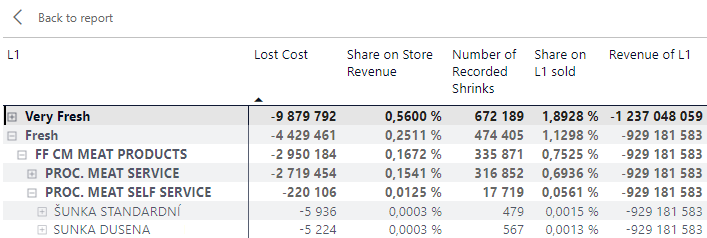
\includegraphics[width=\textwidth]{obrazky/PBI/tabulkaukzka.png}
    \caption{Detail tabulky vybrané ukazatele pro jednotlivé kategorie \\ v~produktové hierarchii.}
    \label{obr:PBI:tab1}
\end{figure}

\subsubsection*{Prodejny}

Další stránka zobrazuje prodejny a k nim příslušné ukazatele. Uživatel může filtrovat prodejny podle typu, kraje nebo okresu. Dále je možné filtrovat také podle kategorií. V~tabulce lze zobrazit údaje agregovaně podle lokalit nebo přímo pro jednotlivé prodejny. Sloupce tabulky jsou rozdělené na hodnoty týkající se malých nebo velkých prodejen a poté celkové hodnoty pro oba typy. Ukázka této stránky je na obr.~\ref*{obr:PBI:stores}.

\begin{figure}[h!]
    \centering
    \captionsetup{justification=centering}
    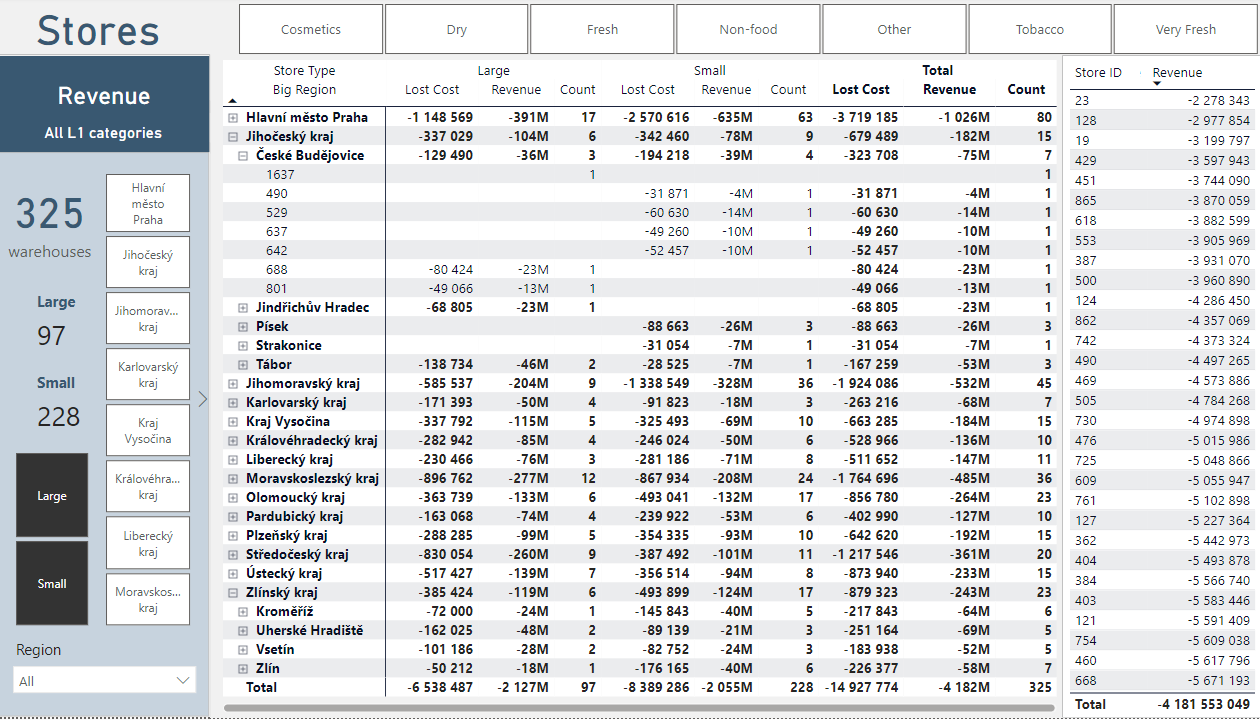
\includegraphics[width=\textwidth]{obrazky/PBI/stores.png}
    \caption{Power BI reporting pro zobrazení údajů o shrincích z~pohledu prodejen.}
    \label{obr:PBI:stores}
\end{figure}

\subsubsection*{Prodejny - Velmi čerstvé a Čerstvé}

Na této stránce reportu jsou vizuály pro analýzu chování shrinků z~hlediska prodejen již pouze pro kategorie Čerstvé a Velmi čerstvé viz obr.~\ref*{obr:PBI:storesSFF}. V~nastavení reportu v~sekci filtrů je možné vybrat i další kategorie, nicméně tato práce se věnuje především analýze těchto dvou kategorií, a tak jsou již předfiltrované tyto kategorie. Opět je možné filtrovat prodejny podle jejich atributů. Také je možné v~horní části stránky vybrat sledovaný shrink (č. 1) -- shrinky jsou pro lepší přehlednost barevně odlišené. 
Stránka dále obsahuje graf č. 2, který vizualizuje zastoupení shrinků podle hodnoty shrinku (tj. ztracené náklady), graf porovnání velkých a malých prodejen podle podílu shrinku na jejich tržbách (č. 3). Pod tímto grafem jsou prodejny porovnané podle jejich ztracených nákladů. Zároveň je datový pruh barevně rozdělený podle typu shrinku (barva je shodná s~barvou shrinku, kterou má přiřazenou nahoře na stránce). 

Graf označený č. 4 zobrazuje ztrátu vlivem shrinku podle velikosti měst, ve kterých se prodejny nachází. Graf umožňuje přejít k podrobnostem, a to typu prodejny a konkrétním prodejnám. Zbylé grafy na stránce zobrazují konkrétní prodejny podle ukazatelů - hodnota shrinku, podíl shrinku na celkových tržbách prodejny, podíl shrinku na tržbách kategorií Velmi čerstvé a čerstvé na sledované prodejně. Grafy jsou rozdělené podle typu prodejen, datové pruhy jsou opět poměrově rozdělené podle zastoupení typů shrinků.

\begin{figure}[h!]
    \centering
    \captionsetup{justification=centering}
    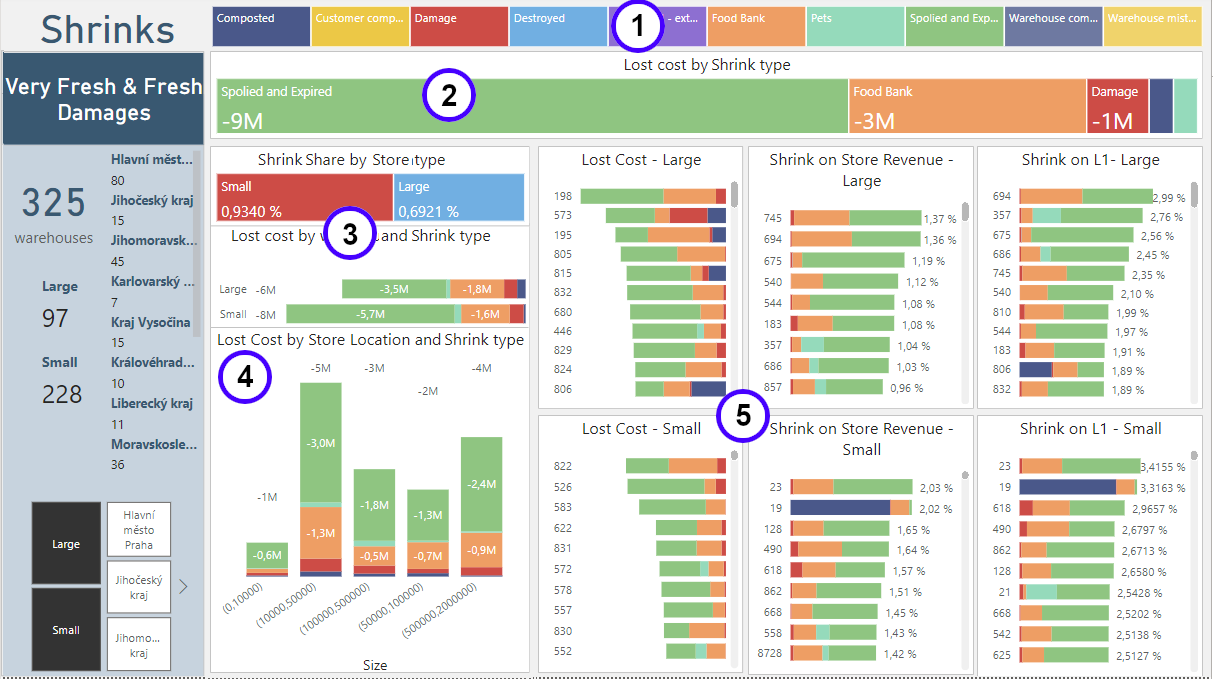
\includegraphics[width=\textwidth]{obrazky/PBI/storesSFF.png}
    \caption{Power BI reporting pro zobrazení údajů o shrincích kategorie \\ Čerstvé a Velmi čerstvé z~pohledu prodejen.}
    \label{obr:PBI:storesSFF}
\end{figure}

\subsubsection*{Kategorie - Velmi čerstvé a Čerstvé}

Další stránka zobrazuje data kategorií Velmi čerstvé a Čerstvé podle dalších příznaků. Grafy označené jedničkou zobrazují podíl shrinku na celkových tržbách z~pohledu typu promoakce a podle kategorie (z libovolné úrovně až k detailu produktu), zároveň je datovým pruhům přiřazeno zastoupení typu shrinku. Tabulka s~č. 2 říká, kolik unikátních produktů bylo shrinkováno podle typu prodejny, od typu jde dá-\\le přejít přes lokaci k samotným prodejnám. Graf č. 3. ukazuje počet záznamů evidovaných v~daný den v~týdnu, legenda zároveň určuje, v~které části měsíce to bylo. 

\begin{figure}[h!]
    \centering
    \captionsetup{justification=centering}
    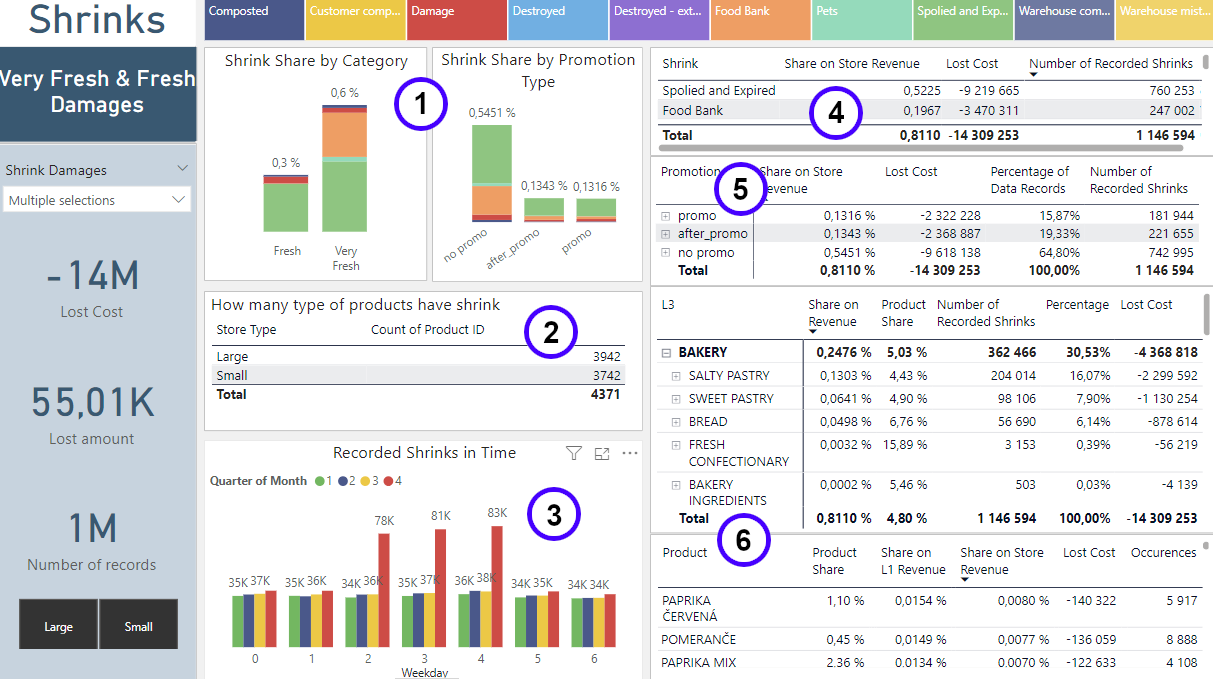
\includegraphics[width=\textwidth]{obrazky/PBI/levelsSFF.png}
    \caption{Zobrazení údajů o shrincích kategorie Čerstvé a Velmi čerstvé \\ se zaměřením na kategorie a produkty.}
    \label{obr:PBI:storesSFF}
\end{figure}

Tabulka č. 4 přiřazuje vybrané ukazatele k jednotlivým typů shrinku. Další tabulka má tyto údaje ale přiřazené podle typu promoakce produktu, který je evidován v~záznamu shrinku. Následující tabulky se týkají již konkrétních kategorií a produktů, z produktu se lze přesunout na další stránku věnující se detailu pouze jednoho produktu (viz obr.~\ref*{obr:PBI:drilldetail}). Sledován je podíl shrinku na tržbách prodejny, na tržbách produktu na prodejne, výskyt v záznamech, ztracená tržba a její procentuální zastoupení. Na stránce jsou i jako v předešlých případech filtry a souhrnné údaje.

\begin{figure}[h!]
    \centering
    \captionsetup{justification=centering}
    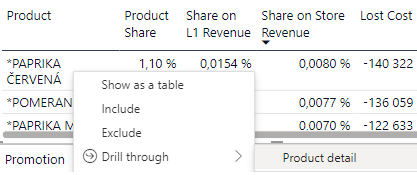
\includegraphics[width=0.45\textwidth]{obrazky/PBI/detaildrill.png}
    \caption{Proklik na stránku s detailem produktu.}
    \label{obr:PBI:drilldetail}
\end{figure}

\subsubsection*{Čas - Velmi čerstvé a Čerstvé}

Na další stránce jsou data porovnávána vzhledem k datumu záznamu -- ke dni v týdnu a části měsíce. Na této stránce, kromě filtrování typů jako v předchozích případech, může uživatel určit pro který ukazatel budou grafy zobrazeny. Vybrat lze ze ztracených nákladů, podílu shrinku na celkových tržbách prodejny a z podílu shrinku na tržbách v dané kategorie a případně v části měsíce, viz č. 1 na obr.~\ref*{obr:PBI:timeSFF}. Zbylé grafy jsou rozděleny na tři části -- podle typu shrinku, podle umístění prodejen a podle typu prodejny. V každé části je přehled, který říká v jakém poměru tyto příznaky jsou (v závislosti na zvoleném ukazateli). Dále jsou pro každou část je ukazatel z pohledu dne v týdnu nebo části měsíce, kdy byl shrink zaznamenán. 

\begin{figure}[h!]
    \centering
    \captionsetup{justification=centering}
    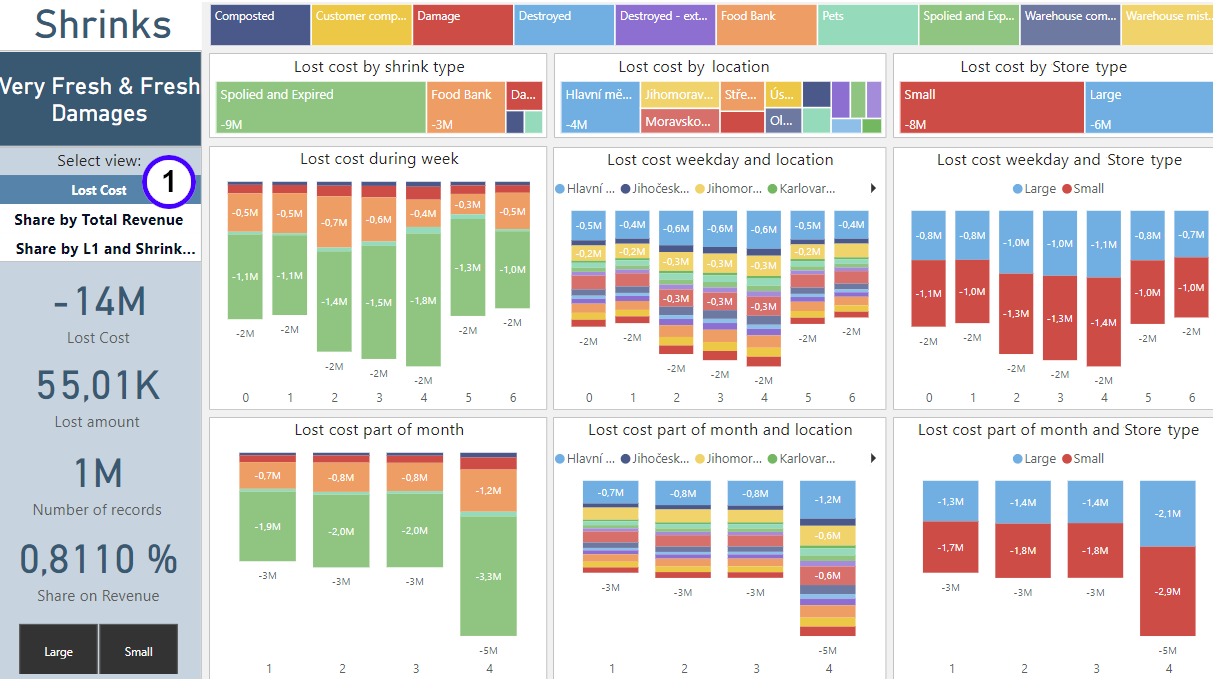
\includegraphics[width=\textwidth]{obrazky/PBI/timeSFF.png}
    \caption{Zobrazení údajů o shrincích kategorie Čerstvé a Velmi čerstvé se zaměřením na časové údaje.}
    \label{obr:PBI:timeSFF}
\end{figure}

\subsubsection*{Detail produktu}

Poslední stránka je věnovaná analýze konkrétního produktu, snímek je na obr. \ref*{obr:PBI:detail}. Je zobrazené zastoupení produktu podel typu prodejny a podle kraje z pohledu ztracených nákladů (č. 1). Dále je na této stránce tabulka (č. 2) se záznamy agregovaná podle data záznamu. Každý řádek s datem lze dále rozbalit pro detail o jaký typ shrinku se jednalo, k jednotlivým řádkům jsou napočítané vybrané ukazatele. Další tabulka (č. 3) ukazuje, jaký podíl na tržbách produktu a celkových tržbách má který typ shrinku. 

Zbylé grafy ukazují konkrétní prodejny, které měli největší podíl shrinku tohoto produktu na svých tržbách, opět celkových i produktových. Dále jak je shrink tohoto produktu rozložený do dní v týdnu, resp. do částí v měsíci (č. 4).

\begin{figure}[h!]
    \centering
    \captionsetup{justification=centering}
    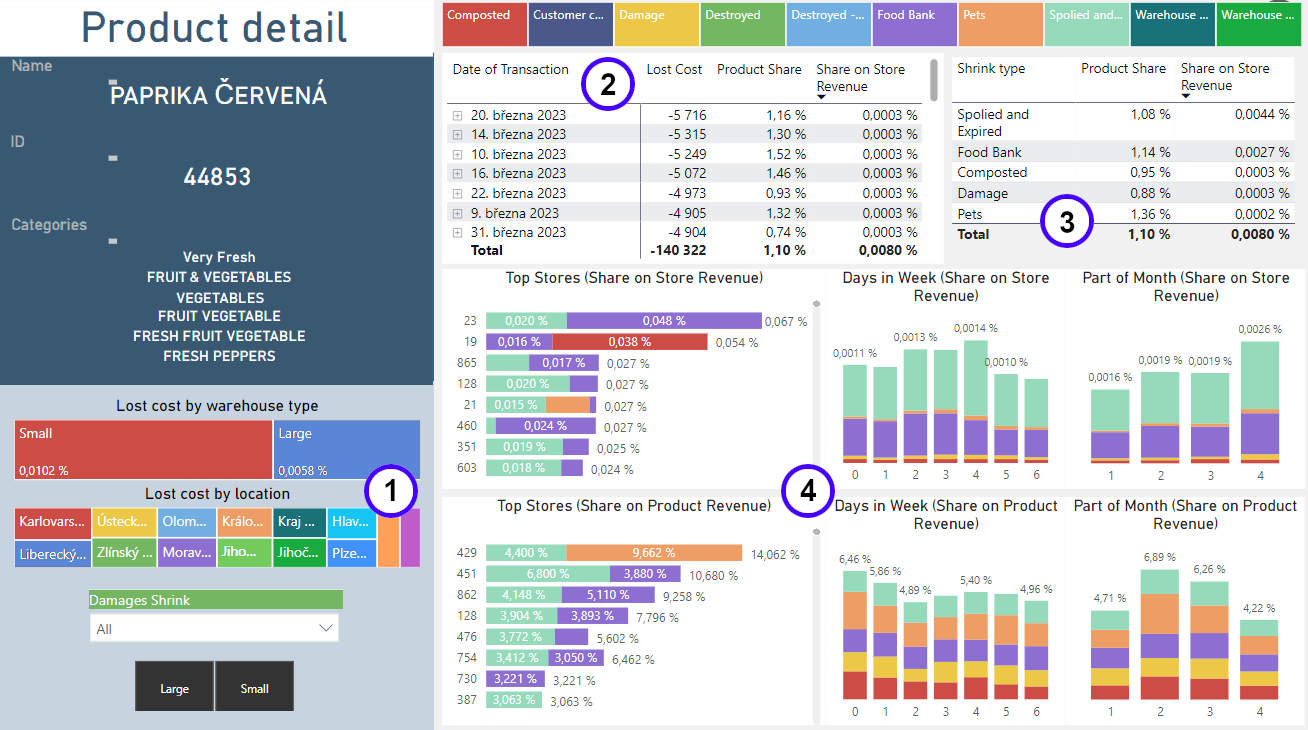
\includegraphics[width=\textwidth]{obrazky/PBI/productdetail.png}
    \caption{Power BI report -- Detail produktu.}
    \label{obr:PBI:detail}
\end{figure}

\section{Výsledky}


\label{sec:vizualizace:vysl}


\chapter{Korelační analýza}
\label{ch:korelacnianalyza}
Tato kapitola se věnuje popisu korelační analýzy pro zjištění důvodu shrinků produktů. Tuto analýzu je možné spustit na data libovolné společnosti, pokud obsahují vstupy, které jsou definované dále. Analýza byla napsána v~jazyce Python, jako sada funkcí sdružená do modulu. Ukázka volání funkcí pro spuštění analýzy je pak vytvořená v~Jupyter Notebooku. V~této kapitole je popsána implementace funkcí a princip analýzy. 

Na základě analýz dat popsaným v sekcích \ref*{sec:priprava}, \ref*{sec:vizualizace:vysl}, \ref*{sec:hypo} nebyl nalezen jednoznačný ukazatel, který by umožnil obecně charakterizovat příčiny vzniku shrinků pouze ze záznamů o jednom produktu. Proto vznikla myšlenka porovnávat zaznamenaný shrink  jednoho produktu s~jinými produkty, konkrétně s~ jejich začleněním do promoakcí v~ daném období a s~tržbami. 
Další analýza proto hodnotí korelaci mezi hodnotou shrinku a tržbami. Na základě získaných výsledků roztřídí produkty ve vstupních datech do několika kategorií, podle toho jaký vliv na ně mají ostatní produkty.

Je důležité mít na paměti, že korelace neznamená kauzalitu. Avšak z~ businessového pohledu na zkoumanou situaci si dovolíme předpokládat, že z~ hodnot korelace mezi sledovanými veličinami lze vyvodit alespoň částečnou příčinu vzniku shrinku produktu.

Pro účely této analýzy bylo potřeba získat z~ databáze tabulku týkající se všech prodejů za měsíc březen roku 2023 bez agregace na prodejny nebo části měsíce. 

% Je možné specifikovat úroveň kategorie, na které se analýza spočítá. Dále je třeba určit konkrétní název kategorie.

% https://mathstat.econ.muni.cz/media/12657/pear_cor.pdf
% https://is.muni.cz/www/98951/41610771/43823411/43823458/44159634/44707073/Pavlik_-_Biostatistika_-_kapitola_11.pdf

% úrovně 4, neboť nižší kategorie ve většině případů produkty již dále nedělí, ale pouze specifikují popis kategorie na   

\section{Postup}
\label{sec:kor:postup}
V rámci analýzy se porovnávají pouze záznamy produktů, které se vyskytují ve stejné kategorii. Jedno pozorování je na agregované na produkt, prodejnu a den záznamu. Základní hypotéza je, že shrink produktu může být ovlivněn promoakcemi jiných produktů v~kategorii.

Hodnotu shrinku jsem porovnávala s~následujícími ukazateli. 
\begin{itemize}
    \itemsep0em 
    \item Tržby daného produktu.
    \item Tržby daného produktu, které byly v~daný den v~promoakci - ukázalo se, že takové, až na výjimky nejsou.
    \item Součet tržeb všech ostatních produktů v~kategorii.
    \item Součet tržeb všech ostatních produktů v~kategorii, které byly v~daný den v~promoakci.
    \item Součet tržeb všech ostatních produktů v~kategorii, které byly v~daný den v~promoakci nebo byly v~rozmezí jednoho týdne po promoakci.
\end{itemize}

Ke každému ukazateli, jsem ještě vytvořila analogický ukazatel, který uvažoval zpoždění shrinku. V~takovém ukazateli, se nebrala hodnota prodeje ze stejného dne, jako byl den záznamu shrinku, ale hodnota z~předchozího dne. Důvodem pro vytvoření takových ukazatelů byla hypotéza, že shrink se může projevit až další den po uskutečněných tržbách. 
%Důvodem může být to, že 

Na základě korelační analýzy je možné roztřídit produkty v~kategorii do šesti skupin:
\begin{itemize}
    \itemsep0em 
    \item[] \textbf{Kategorie P} - Produkty, které si samy způsobují shrink.
    \item[] \textbf{Kategorie O} - Produkty, jejichž shrink je způsoben tím, že ostatní produkty v~kategorii jsou v~promoakci.
    \item[] \textbf{Kategorie X} - Produkty, jejichž shrink se nepodařilo vysvětlit pomocí korelační analýzy.
    \item[] \textbf{Kategorie V} - Produkty, které jsou úspěšné ve výprodejích. Produkt se hodně prodává a zároveň má malé shrinky.
    \item[] \textbf{Kategorie N} - Produkty, jejichž shrink je nezávislý na svých tržbách i tržbách ostatních produktů v~kategorii. Shrink zůstává v~podobném poměru, tj. pokud jsou tržby vyšší je i shrink vyšší, pokud jsou tržby nižší, je nižší i shrink.
    \item[] \textbf{Kategorie F} - Produkty, u nichž nebyl koeficient korelace statisticky významný.
\end{itemize}

Na obrázku \ref*{obr:ctg:g:kategorizace1} je znázorněno rozdělení produktů vzhledem ke korelačnímu koeficientu. Kategorie jsou pro lepší orientaci na obrázku oddělené i barevně, zároveň s~popisem je u každé části i písmenné označení kategorie. 

\begin{figure}[hbtp!]
    \centering
    \captionsetup{justification=centering}
    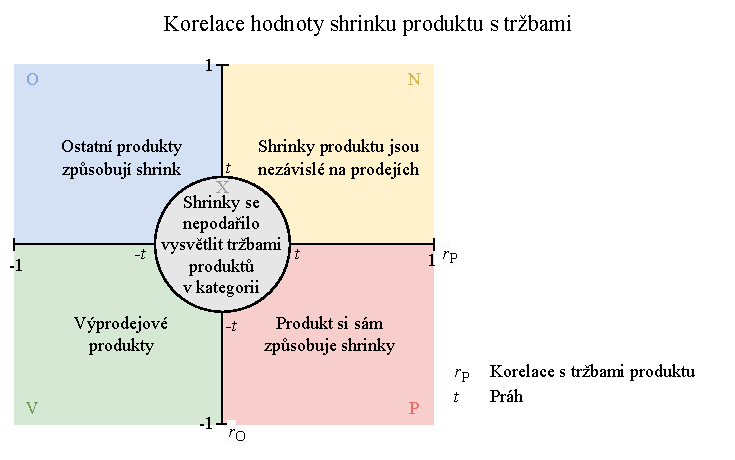
\includegraphics[width=\textwidth]{obrazky/grafy/matice_korelace_typy_DP.pdf}
    \caption{Kategorizace produktů podle korelace hodnoty shrinku s~tržbami.}
    \label{obr:ctg:g:kategorizace1}
\end{figure}

Hypotéza pro zařazení do kategorie P je následující:

Pokud je korelační koeficient zaznamenaného shrinku s~tržbami téhož produktu kladná, produkt si způsobuje shrinky sám.
Abych mohla tuto hypotézu potvrdit, nebo vyvrátit, je třeba statisticky otestovat významnost korelačního koeficientu. Formulovala jsem nulovou hypotézu $H_\mathrm{0}$ a alternativní hypotézu $H_\mathrm{A}$ pro koeficient $r_\mathrm{P}$, který měří korelaci mezi hodnotou shrinku a tržbami produktu.

\begin{equation*}
    \begin{aligned}
        H_\mathrm{0}: \quad & r_\mathrm{P} = 0 \qquad \mbox{Výběry nejsou korelované.}  \\
        H_\mathrm{A}: \quad & r_\mathrm{P} \neq 0 \qquad\mbox{Výběry jsou korelované.}\\
    \end{aligned}
\end{equation*}

Hypotéza pro zařazení do kategorie O je následující:

Pokud jsou kladně korelované hodnoty zaznamenaného shrinku a tržby ostatních produktů a zároveň korelace shrinků produktu s~vlastními tržbami je záporná, potom lze vyslovit hypotézu, že shrinky na produktu jsou způsobené ostatními produkty v~promoakci.
Pro toto tvrzení je opět nutné statisticky otestovat koeficienty korelace. Pro koeficient $r_\mathrm{P}$ je statistický test stejný jako v~předchozím případě. Pro koeficient $r_\mathrm{O}$ měřící, jak jsou korelované shrinky a tržby ostatních produktů, je třeba otestovat následující hypotézy.
\begin{equation*}
    \begin{aligned}
        H_\mathrm{0}: \quad & r_\mathrm{O} = 0 \qquad \mbox{Výběry nejsou korelované.}  \\
        H_\mathrm{A}: \quad & r_\mathrm{O} \neq 0 \qquad\mbox{Výběry jsou korelované.}\\
    \end{aligned}
\end{equation*}

Pokud na zvolené hladině významnosti zamítneme nulovou hypotézu pro zkoumané korelační koeficienty, můžeme tvrdit že s~danou pravděpodobností je koeficient statisticky významný. Na základě hodnoty korelace lze pak produkt zařadit do příslušné kategorie. Produkty, u kterých nelze zamítnout, není možné zařadit do tří uvedených kategorií.

Pro výpočet korelačního koeficientu je ještě třeba ověřit předpoklady. Pro Pearsonův korelační koeficient se jedná o~předpoklad normality dat, shodnost rozptylů a nezávislost dat. Pro Spearmanův korelační koeficient není třeba splňovat tyto předpoklady.

\section{Implementace}

V~této části je uveden přesný postup pro získání kategorizace produktů. Kód je napsaný v~jazyce Python verze 3.9. Součástí kódu je výběr kategorií, které jsou zkoumány, propojení dat shrinků, prodejů a promoakcí, výpočet korelace a ověření předpokladů, statistické testování a rozřazení produktů.

% UML diagram pro analýzu.

\subsection{Vstupy a výstupy}
\label{ss:vstupyvystupy}

Pro korelační analýzu zaznamenaných shrinků s~tržbami dalších produktů je třeba zajistit data, které se týkají zaznamenaných prodejů, produktů a~prodejen. V násle-\\dující části jsou popsány tabulková data, která jsou nezbytná pro správné spuštění analýzy. Dále jsou definované i vstupy, které musí definovat uživatel pro specifikování názvů konkrétních sloupců v~souborech a parametry pro analýzu.

Celkem jsou požadovány čtyři vstupní tabulky - \emph{záznamy shrinků, záznamy prodejů, záznamy o~promoakcích, číselník produktů s~rozdělením produktové hierarchie}. %a~rozdělení prodejen.
Tabulka se zaznamenanými shrinky musí obsahovat sloupec s~datem záznamu, ID produktu, ID prodejny, hodnotu zaznamenaného shrinku. Tabulka s~prodeji potřebuje stejné sloupce jako tabulka se shrinky s~výjimkou že hodnota prodejů je celková prodaná částka, která byla zaznamenaná na dané prodejně v~jeden den u daného produktu. Tabulka s~údaji o promoakcích by měla obsahovat ID produktu, kterého se promoakce týká, začáteční a koncové datum promoakce a ID prodejny, pro kterou promoakce platí.
Všechny záznamové tabulky musí pokrývat stejné časové období. Období může být libovolně dlouhé.
Tabulka produktové hierarchie obsahuje ID produktu, jeho název a libovolně hluboký strom hierarchií. Každá úroveň stromu má vlastní sloupec. Všechny úrovně jsou vyplněné pro každý produkt, tato podmínka je nutná jen pro kategorie, které bude chtít uživatel využít při analýze. 
Tabulka s~hierarchií produktů slouží k~tomu, aby mohla být napojena na ostatní tabulky a data se pak mohla vyfiltrovat pouze na záznamy týkající se vybrané kategorie.

Před spuštěním hlavní výpočetní části musí uživatel vypsat konkrétní pojmenování sloupců v~tabulce do proměnných. Sloupce, které v~různých tabulkách označují tytéž hodnoty, musí mít stejný název. 
% V~následujícím kódu \ref*{code:colnames} je ukázka zadání.
 V~komentářích je slovní popis o jaký sloupec se jedná. Sloupec by však měl být jasný přímo z~názvu proměnné.

% \begin{lstlisting}[language=Python, style=mystyle, label={code:colnames}, caption={Definice konkrétních názvů sloupců.}]
% product_col      = "product_id"             # Product ID column
% product_name_col = "name"                   # Product name column
% whs_id_col       = "warehouse_id"           # Store ID column
% date_col         = "date_of_transaction"    # Date of transactions column - for sales and shrinks tables
% value_col_shrink = "cost_value"             # Column with value of shrinks (shrink table)
% value_col_sales  = "cost_value"             # Column with value of total sales (sales table)
% promo_col_from   = "promotion_date_from"    # Starting date of promotion (promotion table)
% promo_col_to     = "promotion_date_to"      # Starting date of promotion (promotion table)
% categories       = ["L3","L4","L5","L6", "name"]  # Categories that we want to map to product ID (product hierarchy) 
% \end{lstlisting}

Uživatel dále zadefinuje formát data, který se používá v~datumových sloupcích, aby se tyto sloupce mohly převést z~textového řetězce na typ \texttt{datetime}. V~proměnné \texttt{category\_column} je třeba vybrat jednu kategorii (název sloupce). Na této úrovni se poté budou procházet jednotlivé kategorie, v~rámci každé z~nich se pak budou porovnávat a třídit produkty. V~dalších proměnných může uživatel změnit umístění tj. název složky, kam se ukládají výsledky kategorizace a grafy. Složky s~těmito názvy se vytvoří jako podsložky aktuální cesty.

% \begin{lstlisting}[language=Python,style=mystyle,, label={code:params},  caption={Definice parametrů.}]
% date_format = "%Y-%m-%d"                    # Format of date columns
% category_column = "L6"                      # Level od product hierarchy, on which to compare products (have to be in categories)
% \end{lstlisting}

\subsection{Spuštění analýzy}

Analýzu lze spustit pomocí předpřipraveného Jupyter Notebooku v~jazyce Python. V~první buňce notebooku se načítají potřebné balíčky a modul s~definovanými funkcemi pro analýzu.

V dalším buňce jsou definovány vstupní parametry do funkcí - názvy sloupců a úrovně produktové hierarchie.
V následující buňce se načítají potřebné datasety. Přehled potřebných vstupů je v~sekci \ref*{ss:vstupyvystupy}. V~závislosti na konkrétních datech je třeba specifikovat, jak se mají tabulková data načíst - jedná se např. o parametry pro oddělovač hodnot v~řádku, nebo značení desetinné čárky v~datech. Pokud nahrané datasety pro prodeje, shrinky a promoakce mají pouze sloupec ID produktu s~nenapojenou produktovou hierarchií, je třeba ji připojit.

V další buňce se spouští samotná analýza. Nejprve se spustí funkce, která vrátí seznam kategorií, které jsou nejrizikovější. Je třeba definovat na které úrovni hierarchie se budou kategorie prohledávat a také, kolik kategorií budeme chtít prozkoumat.
Nalezené kategorie se dále prochází v~cyklu.

Z datasetů se vyfiltrují pouze záznamy dané kategorie. Pokud jsou v~prodejích záznamy, kde je prodej kladný, tak se tyto záznamy vynechají. V~dalším kroku se k~údajům o prodejích navážou promoakce. Poté je spuštěna korelační analýza, lze definovat, jaká metoda se má použít s~jakou alternativní hypotézou. Případně zda uživatel chce zkoumat shrinky oproti zpožděným prodejům a zda se má analýza zabývat pouze promočními prodeji, nebo i popromočními.

Vypočítané korelační koeficienty se kategorizují a výsledky se uloží do souboru. Zároveň se pro zkoumanou kategorii uloží i graf závislosti shrinků na promočních prodejích.


\subsection{Popis funkcí a struktura kódu}

Kód pro korelační analýzu je umístěn ve složce \texttt{shrink\_categorization}, struktura složky je vidět na obrázku \ref*{obr:strukturaslozky}.

\begin{figure}[hbtp!]
    \captionsetup{justification=centering}
    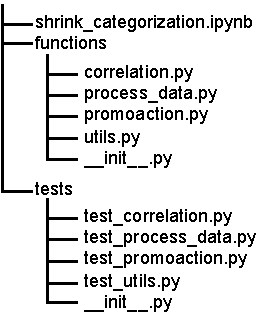
\includegraphics[width=.3\textwidth]{obrazky/strukturaslozky.pdf}
    \caption{Struktura souborů pro kód zpracovávající korelační analýzu.}
    \label{obr:strukturaslozky}
\end{figure}

Funkce jsou rozčleněny do modulů podle toho, na jaký výpočet jsou zaměřené. Každá funkce má je zdokumentovaná pomocí docstring obsaženého ve své definici. Dokumentace funkce se skládá ze stručného popisu, co funkce dělá, jaké má vstupní parametry a jaký je jejich význam a co funkce vrací. Funkce jsou otestované pomocí unit testů.

Pro práci s~tabulkovými daty, které jsou hlavním vstupem, jsem použila balíček \emph{pandas} jazyka Python. 
Pro otestování důležitých funkcí jsem použila knihovnu \emph{pytest}. 


% \emph{V~závorce je nástin toho, co budu popisovat (TBD)}

% \begin{itemize}
%     \item Výběr kategorie (Aby se nemuselo zadávat, přesné názvy kategorií systém vybere prvních $n$ nejsilnějších kategorií z~pohledu shrinků.)
%     \item Propojení dat
%     \item Korelace (Pearsonův, Spearmanův korelační koeficient) (ověření předpokladů (Kolmogorov-Smirnov test pro IID), testování statistické významnosti)
%     \item Kategorizace (Nastavení prahu pro velikost korelačního koeficientu)
%     \item Pomocné funkce
% \end{itemize}

\subsubsection*{Funkce pro přiřazení kategorií k~produktům}

Jak je uvedeno na začátku sekce \ref*{ss:vstupyvystupy}, uživatel musí specifikovat názvy sloupců kategorií, které bude v~analýze používat. Seznam těchto kategorií je pak parametrem pro funkci \texttt{assign\_levels}. Další parametry jsou DataFrame, kam se mají kategorie napojit a DataFrame odkud se kategorie napojují. Tyto DataFramy musí mít společný sloupec, podle kterého se napojení provede. Defaultně se jedná o sloupec s~ID produktu. Defaulně se provádí \emph{left join}, aby nedošlo ke ztrátě dat, kdyby nějaký produkt neměl v~DataFramu kategorií zastoupení. Funkci je také možné předat další argumenty, které se dají volat ve funkci \texttt{merge} knihovny \emph{pandas}. V~analýze shrinků jeden řádek dat odpovídá transakci jednoho produktu, proto byl zvoleno ID produktu jako propojovací sloupec.

\subsubsection*{Funkce pro vytipování rizikových kategorií}

Funkce \texttt{define\_risk\_categories} vybere prvních $n$ kategorií v~dané produktové hierarchii, kde suma hodnot v~dané kategorii, je nejvyšší, resp. nejnižší. Funkce vrací seznam těchto kategorií. Prvním vstupní parametrem je DataFrame, který obsahuje minimálně tři sloupce. Tyto sloupce je třeba definovat jako další parametry funkce. Jedná se o~sloupec \texttt{value\_column}, ve kterém jsou hodnoty, které ohodnocují řádky DataFramu a kategorie. Další sloupec je jedna z~úrovní produktové hierarchie, ve sloupci se nachází názvy, nebo jiné označení, kategorií. Posledním povinným parametrem je počet kategorií, které má funkce vrátit. Pokud je zadán tento počet tak, že je větší než je počet unikátních kategorií, vrátí se všechny kategorie seřazené od nejrizikovější. Dale je funkci možné předat keyword argumenty, které se předají funkci \texttt{sort\_values} z~knihovny \emph{pandas}. Jedná se např. o~parametr pro vzestupné, nebo sestupné řazení. Defaultní řazení je vzestupné, což znamená, že se vezmou kategorie s~nejnižší hodnotou. V~této analýze sledujeme vyhozené množství, resp. peníze. Tento ukazatel je záporný, tedy vzestupné řazení vybere ty kategorie, jejichž ztráta byla nejvyšší. Vrácený seznam kategorií je tedy seřazen od nejrizikovější kategorie.

\subsubsection*{Funkce pro výběr pouze dané kategorie ze všech záznamů}
Ve funkci \texttt{select\_category} jsou vstupem DataFrame, název kategorie a úroveň, ve které se daná kategorie nachází. Funkce vrací DataFrame pouze s~těmi řádky, kde je obsažena jmenovaná kategorie. V~případě, že tato kategorie v~datech není, je vrácen prázdný DataFrame.

Tato funkce je volána ve funkci \texttt{process\_dataframes}. Vstupy jsou totožné, avšak namísto jednoho DataFramu je možné jich zadat více jako samostatné parametry. 
% Tělo funkce je v~kódu \ref*{code:processdf}. 
Funkce vrací seznam všech vstupních DataFramů, a to pouze řádky, které obsahují zadanou kategorii.

% \begin{lstlisting}[language=Python,style=mystyle, label={code:processdf},  caption={Funkce pro výběr pouze dané katageorie z~více DataFramů.}]
% def process_dataframes(category: str, category_column: str, *dataframes) -> list[pd.DataFrame]:
%     result_dataframes = []

%     print("Sizes of dataframes: ")

%     for df in dataframes:
%         result_df = select_category(df, category, category_column)
%         print("Shape of original df: " , df.shape, "Shape of new df: " , result_df.shape)
%         result_dataframes.append(result_df)

%     return result_dataframes
% \end{lstlisting}

\subsubsection*{Funkce pro přiřazení promoakcí}

V rámci korelační analýzy bylo potřeba přiřadit k~jednotlivým zaznamenaným transakcím, zda byl produkt v~den záznamu v~promoakci nebo nikoli. V~ideálním případě by tento příznak mohl být již uvedený u každého záznamu. Pokud tomu tak, ale není, je nutné data o promocích provázat na základě data, produktu a prodejny podle číselníku promoakcí. Data vybrané společnosti, na jejíchž datech analýza probíhá, nemají promoakce přímo napojené na již proběhlé, zaznamenané transakce. Data o promoakcích jsou uložená v~číselníku promoakcí. Ten obsahuje ID produktu, prodejny, začátek a konec promoakce a prioritu promoakce. V~jeden den může být více promoakcí, v~takovém případě platí ta s~nejvyšší prioritou.

Základní funkce pro přiřazování promoakcí k~záznamům s~transakcemi se nazývá \texttt{map\_all\_promotions}. Tato funkce propojí DataFrame s~promoakcemi s~druhým DataFramem s~transakcemi. Může se jednat jak o záznamy shrinků, tak i o~prodeje. Důležité je, že tento DataFrame má sloupec s~datem, protože díky datu pak lze identifikovat správnou promoakci. Nalezení správné promoakce je implementováno až ve funkci \texttt{promo\_}, viz dále v~této sekci. Funkce \texttt{map\_all\_promotions} nejprve provede vnitřní spojení (neboli \emph{inner join}) obou vstupních DataFramů podle definovaných sloupců v~parametrech funkce. Tyto sloupce jsou vzhledem k~datům společnosti - sloupce s~ID produktu a ID prodejny. Tím je docíleno toho, že z~promoakcí získáme pouze ty záznamy pouze těch produktů, které se prodali, a které zároveň byly v~promoakci. Duplicitní záznamy se vynechají. U každého takového záznamu spočítá, kolikrát byl k~němu byla přiřazeno promoakce (tj.~kolik bylo promoakcí ve sledovaném období pro daný produkt a prodejnu) a ke~každému záznamu toto číslo přiřadí. Spolu s~číslem se přiřadí i identifikátor promoakce pro dvojici produkt-prodejna (viz tabulka C), tím je určena skupina k~sobě patřících záznamů. Takto označené záznamy se připojí k~původnímu DataFramu s~transakcemi. Záznamy, kde není žádná promoakce je počet promoakcí roven nule, zbylé hodnoty nejsou definované.
Dále se identifikátor upraví tak, že dokáže rozlišit unikátní promoakci na trojici produkt-prodejna-datum (viz tabulka D). V~tabulce \ref*{tab:tabulkypromoakceukaz} jsou umělá ukázková data, na kterých je znázorněno spojování dat.

\begin{table}[hbtp!]
    \centering
    \captionsetup{justification=centering}
    \caption{Umělá data pro znázornění přiřazování promoakcí k~transakcím.}
    \begin{tabular}{llll}
    \multicolumn{4}{c}{Tab. A: Tabulka promoakcí } \\
    \toprule
    ID produktu & Prodejna & Začátek promoakce & Konec promoakce  \\
    \midrule
    0001 & 01 & 2023-03-01 & 2023-03-05 \\
    0001 & 01 & 2023-03-15 & 2023-03-25 \\
    0002 & 02 & 2023-03-15 & 2023-03-25 \\
    0003 & 10 & 2023-03-15 & 2023-03-25 \\
    0004 & 02 & 2023-03-15 & 2023-03-25 \\
    \bottomrule
    \end{tabular}
\bigskip
    \begin{tabular}{lll}
        \multicolumn{3}{c}{Tab. B: Tabulka transakcí} \\
        \toprule
        Produkt & Prodejna & Datum transakce  \\
        \midrule
        0001 & 01 & 2023-03-02  \\
        0001 & 01 & 2023-03-09  \\
        0002 & 02 & 2023-03-15 \\
        0003 & 02 & 2023-03-15 \\
        0004 & 10 & 2023-03-15 \\
        0004 & 11 & 2023-03-30 \\
        \bottomrule
    \end{tabular}
\bigskip
    \begin{tabular}{llp{2cm}p{2.2cm}p{2cm}p{2cm}}
        \multicolumn{6}{c}{Tab. C: Tabulka souhlasných dvojic promoakce-produkt} \\
        \toprule
        Produkt & Prodejna & Začátek promoakce & Konec \newline promoakce& Identifikátor dvojice & Počet \newline  promoakcí\\
        \midrule
        0001 & 01 & 2023-03-01 & 2023-03-05 & 1 & 2\\
        0001 & 01 & 2023-03-15 & 2023-03-25 & 1 & 2\\
        0002 & 02 & 2023-03-15 & 2023-03-25 & 2 & 1\\
        \bottomrule
    \end{tabular}
\bigskip
    \begin{tabular}{llp{2cm}p{2cm}p{2.1cm}p{1.2cm}p{1.3cm}}
        \multicolumn{7}{c}{Tab. D: Tabulka souhlasných trojic promoakce-produkt-datum} \\
        \toprule
        Produkt & Prodejna & Datum transakce & Začátek promoakce & Konec \newline promoakce& Identi-\par fikátor trojice & Počet \newline promo-\par akcí\\
        \midrule
        0001 & 01 & 2023-03-02 & 2023-03-01 & 2023-03-05 & 1A & 2 \\
        0001 & 01 & 2023-03-02 & 2023-03-15 & 2023-03-25 & 1A & 2 \\
        0001 & 01 & 2023-03-09 & 2023-03-01 & 2023-03-05 & 1B & 2 \\
        0001 & 01 & 2023-03-09 & 2023-03-15 & 2023-03-25 & 1B & 2 \\
        0002 & 02 & 2023-03-15 & 2023-03-15 & 2023-03-25 & 2A & 1 \\
        0003 & 10 & 2023-03-15 & NaN & NaN & NaN & 0 \\
        0004 & 10 & 2023-03-15 & NaN & NaN & NaN & 0 \\
        0004 & 11 & 2023-03-30 & NaN& NaN & NaN & 0 \\
        \bottomrule
    \end{tabular}
    \label{tab:tabulkypromoakceukaz}
\end{table}

Z ukázky a z~popsaného postupu plyne, že výsledný DataFrame může mít více řádků než ten původní, ke kterému se přidávali promoakce. V~dalším kroku je tedy potřeba určit, která z~přiřazených promoakcí probíhala ve stejný čas jako je čas transakce. K~tomu jsem vytvořila funkci \texttt{label\_date\_with\_promo}. V~této funkci je každý řádek promoakce označen jednou ze tří možností: \texttt{no promo, promo, after promo}. Tedy zda je datum transakce během promoakce, nebo nikoli, nebo zda je v~rozmezí týden po evidované promoakci. Vzniklý příznak byl pojmenován jako typ promoakce. Ve~funkci se pracuje pouze se záznamy u nichž byla nalezena alespoň jedna možná promoakce, tj. transakce, kde dvojice produkt-prodejna existuje i v~promoakcích. Zbylé řádky tato funkce neoznačuje. V~tabulce \ref*{tab:tabulkalabely} jsou podle těchto pravidel označené jednotlivé řádky\footnote[1]{Zbylé sloupce jsou vynechané, protože pro ukázku příznaku nejsou podstatné.}.
 
\begin{table}[hbtp!]
    \centering
    \captionsetup{justification=centering}
    \caption{Tabulka transakcí a promoakcí s~přidaným příznakem typ promoakce.}
    \begin{tabular}{llp{2cm}p{2.1cm}p{2cm}p{2.5cm}}
        \toprule
        Produkt & Prodejna & Datum transakce & Začátek promoakce & Konec \newline promoakce& Typ \newline promoakce\\
        \midrule
        0001 & 01 & 2023-03-02 & 2023-03-01 & 2023-03-05 & promo \\
        0001 & 01 & 2023-03-02 & 2023-03-15 & 2023-03-25 & no promo \\
        0001 & 01 & 2023-03-09 & 2023-03-01 & 2023-03-05 & after promo \\
        0001 & 01 & 2023-03-09 & 2023-03-15 & 2023-03-25 & no promo \\
        0002 & 02 & 2023-03-15 & 2023-03-15 & 2023-03-25 & promo\\
        0003 & 10 & 2023-03-15 & NaN & NaN & no promo \\
        0004 & 10 & 2023-03-15 & NaN & NaN & no promo \\
        0004 & 11 & 2023-03-30 & NaN & NaN & no promo \\
        \bottomrule
    \end{tabular}
    \label{tab:tabulkalabely}
\end{table}

V dalším kroku je třeba vybrat pouze jednu přiřazenou promoakci o to se stará funkce \texttt{find\_duplicated\_records}. Tato funkce vrací seznam indexů řádků DataFramu, které se mohou zahodit. Algoritmus je znázorněný na obr. \ref*{label} \emph{TBD: obrázek UML}.
Postupně se prochází každý řádek DataFramu. v~pomocné proměnné se zaznamenává aktuální identifikátor určující jednoznačnou trojici produkt-prodejna-datum. Nejdříve se do pomocného seznamu nahrají všechny indexy řádků, které mají aktuální identifikátor. Potom se iteruje přes všechny tyto vybrané řádky. Pokud je typ promoakce iterovaného řádku typu \texttt{promo}, běh se zastaví a tento řádek se vybere ze skupiny záznamů, uloží se a pokračuje se na další skupinu. Pokud typ promoakce nebyl \texttt{promo}, ale \texttt{after promo}, tak se vybere tato promoakce, následné kroky jsou analogické předchozímu případu. Pokud nenastala ani jedna z~možností zbývá situace, kdy typ promoakce je \texttt{no promo}. Až jsou takto prohledané všechny záznamy, na základě seznamu vybraných řádkových indexů se vytvoří seznam indexů ke smazání jako rozdíl všech indexů v~DataFramu a indexů s~vybranými promoakcemi.

Funkce \texttt{match\_promo\_to\_sales} sdružuje dříve popsané funkce, které zpracovávají promoakce. Vstupními parametry funkce jsou DataFramy transakcí a promoakcí a názvy sloupců. Názvy sloupců mají předdefinovanou hodnotu, kterou lze změnit. v~dalším volitelném parametru je možné specifikovat formát datumu. Všechny slou-\\pce obsahující datumy se převedou na typ \texttt{datetime}. Poté se zavolá funkce \texttt{map\_all\_\\promotions}, která spojí transakce s~promoakcemi. Může vzniknout DataFrame, který má více řádků než původní. Výsledný DataFrame se předá funkci \texttt{label\_date\_\\with\_promo}, kde se označí u napojených promoakcích typ promoakce. Dále se pomocí funkce \texttt{find\_duplicated\_records} vyberou všechny řádky, které obsahují redundantní záznamy. Tyto řádky se odstraní z~DataFramu s~namapovanými promoakcemi. Ke všem řádkům, ke kterým neexistuje promoakce v~číselníku promoakcí, je přiřazen příznak \texttt{no promo}. Na závěr funkce zobrazí souhrn o velikostech dílčích DataFramů, aby měl uživatel informaci o počtech duplicitních záznamů. Během výpočtu jsou procesy iterování sledovány pomocí knihovny \emph{tqdm}.

\subsubsection*{Funkce pro korelační analýzu}

Funkce \texttt{aggregate\_sum} je pomocná funkce použitá v~kategorizaci produktů. Funkce zagreguje vstupní DataFrame podle uvedených sloupců a sečte hodnoty ve všech numerických sloupcích. Ve~výsledném DataFramu resetuje označení řádků a vrátí ho.

Hodnoty korelačních koeficientů se počítají ve funkci \texttt{correlation}. Funkci je předán DataFrame a sloupce, kterých se korelace týká. Tato analýza je zaměřena na korelaci hodnoty shrinku s~dalšími ukzateli, proto je jedním vstupem název sloupce se shrinky a dalším vstupem je seznam sloupců ostatních ukazatelů. Obecně se nemusí jednat o~sloupec shrinků, základní myšlenkou ale je, že korelace je počítána pro každý sloupec ze seznam sloupců s~právě tímto jedním shrink sloupcem. Jedním z~volitelných parametrů funkce je určení metody pro získání korelačního koeficientu. Implementovány jsou dvě metody Pearsonův korelační koeficient a Spearmanův korelační koeficient. Pro výpočet jsou využité metody z~knihovny \emph{scipy}. Těmto metodám lze předat argument, zda se má uvažovat jednostranná nebo oboustranná alternativní hypotéza. Defaultní metodou je Pearsonův korelační koeficient a oboustranná alternativní hypotéza \cite{bib:scipyPearson}.

Před spuštěním výpočtů korelací jsou sloupce testované pro předpoklady IID. Pro testování, zda dva zkoumané sloupce patří do stejného rozdělení byl použitý Kolmo-\\gorov-Smirnovův test implementovaný v~knihovně \emph{scipy}. Pro nezávislost Ljung-Boxova metoda implementovaná v~knihovně \emph{statsmodels}.

Pro každý vypočtený koeficient je spočtena i $p$-hodnota, díky které lze hodnotu koeficientu označit za statisticky významnou, nebo ne. Pro určení významnosti byla implementována pomocná funkce \texttt{significance}. Ta vrací \texttt{True}, resp. \texttt{False} pro statisticky významné, resp. nevýznamné výsledky, tedy pokud je $p$-hodnota menší, resp. větší než $\alpha$. Předpokládaná hladina významnosti $\alpha$ je 5~\%. Výši hladiny lze změnit v~parametru funkce pro výpočet korelace, odtud se předá funkci pro určení významnosti. Vypočtené koeficienty a boolovský příznak o jejich významnosti se ukládají do dvou seznamů, které funkce vrací. Oba seznamy mají takový počet hodnot, jaká je délka vstupního seznamu sloupců.

V parametru \texttt{days} funkce \texttt{correlation} lze specifikovat, zda se má  korelace spočítat pouze mezi sloupcem shrinků se všemi sloupci ze seznamu sloupců anebo navíc se všemi sloupci ze seznami, kde jsou ale hodnoty v~tomto sloupci posunuté o parametr \texttt{days}. Pokud například \texttt{days=1}, pak k~hodnotě shrinku zaznamenané v~jistý den nebude náležet hodnota prodejů v~témže dni, ale hodnota ze dne předchozího. Tato volba byla přidána na základě hypotézy, že shrink se může projevit se zpožděním. Pokud jsou data takto posunutá, je třeba nahradit data na začátku sledovaného období. 
% v~současné implementaci jsou data nahrazená nulou, do budoucna by mohla být zvolena vhodná 

Funkce \texttt{product\_sales\_correlation} je zastřešující funkcí pro korelační analýzu na datových vstupech. Vstupními daty jsou DataFrame se záznamy shrinků a se záznamy prodejů včetně informace o promoakcích. K tomu je třeba definovat názvy  sloupců potřebných pro analýzu. Jedná se o sloupec s~hodnotami shrinků, hodnotou prodejů, ID produktů, ID prodejen a daty transakcí. Názvy sloupců mají defaultní hodnotu, kterou je samozřejmě možné změnit podle zkoumaných dat. Dále má funkce volitelný parametr \texttt{after\_promo}, jehož defaultní hodnota je \texttt{False}, který zohledňuje, zda se pro analýzu s~promočními prodeji použijí jen prodeje uskutečněné přímo během promoakce nebo i prodeje, které nastaly týden po promoakci. Další parametry jsou volitelné parametry, které se předávají funkcím, které jsou volány v~rámci zastřešující funkce (metoda, alternativní hypotéza, hladina významnosti, počet dní posunu). 

Funkce vrací tři proměnné. První je DataFrame, který obsahuje seznam produktů a ke každému z~nich napočítané korelační koeficienty hodnoty shrinku s~ukazateli a statistickou významnost tohoto koeficientu. Déle je vrácen seznam produktů, které neměly žádný promoční prodej ve sledovaném období a případně i produktů, které neměly žádný prodej.

Funkce nejprve vytiskne hlášku, která metoda pro výpočet korelace se použije. Poté se inicializují názvy sloupců pro ukládání korelací a příznaku o statistické významnosti. Počet sloupců se liší v~závislosti na tom, zda se v~analýze zkoumá i varianta se zpožděním shrinku oproti prodejům. Sloupce jsou seřazené tak, aby sloupce týkající se korelace s~jedním ukazatelem byly vedle sebe v~následujícím pořadí: korelační koeficient, statistická významnost, korelační koeficient se zpožděním, statistická významnost pro koeficient se zpožděním. Takto budou hodnoty uložené ve výsledném DataFramu. Pro všechny ukazatele se čtveřice (v případě zpoždění) nebo dvojice (bez zpoždění), opakuje. Dále se inicializuje prázný DataFrame pro ukládání výsledků s~názvem sloupce pro ID produktu spolu s~nově vytvořenými názvy. 

Dále je třeba ze vstupního DataFramu prodejů vybrat pouze záznamy produktů, které se prodaly během promoakce. Pokud je parametr \texttt{after\_promo} je \texttt{True}, pak se kromě záznamů produktů v~promoakci vyberou i ty, kde produkty byly prodány v~rámci týdne po promoakci. Dále se inicializují prázdné seznamy pro uchování produktů, které nemají žádné prodeje, resp. promoční prodeje.

Následně probíhá iterace přes všechny unikátní produkty, pro které byl zaznamenaný shrink. Počet zkoumaných produktů se vytiskne. Na začátku každé iterace je třeba z~DataFramů shrinků vybrat pouze záznamy s~daným produktem. DataFrame se potom agreguje podle sloupců datum transakce a ID prodejny. Stejný postup se aplikuje pro DataFrame s~prodeji. Navíc se obdobný postup aplikuje i na DataFramy s~promočními záznamy a se všemi prodeji s~tím rozdílem, že se vyhledají záznamy všech produktů kromě iterovaného produktu. Výsledné DataFramy se potom sloučí do jednoho podle sloupců ID prodejny a datumu. Jelikož může nastat situace, že ne všechny hodnoty jsou definované na každém řádku, nahradí se nedefinované hodnoty nulou.

Na složený DataFrame se použije funkce \texttt{correlation}, které se předají příslušné parametry. Výsledky se pak vloží jako nový řádek do DataFramu pro ukládání výsledků. Pokud nebylo možné spočíst korelace, z~důvodu, že rozptyl hodnot byl nulový - nastane pokud produkt nemá žádné prodeje -  nahradíme nedefinovanou korelaci nulou, která indikuje, že mezi veličinami není závislost.

Výsledný DataFrame s~korelací je vstupem do funkce \texttt{categorization}.  Dalšími vstupy je název sloupce, který obsahuje korelačními koeficienty shrinků produktu s~jeho vlastními tržbami a sloupce s~koeficienty shrinků produktu s~prodeji ostatních produktů. Ve funkci se vytvoří nový DataFrame pro uložení výsledků kategorizace. Jeho indexem jsou ID produktů. Samotná kategorizace se získá spuštěním funkce \texttt{categorize\_products}, která vrací seznam kategorií pro každý řádek vstupního DataFramu. Funkce \texttt{categorize\_products} roztřídí produkty do pěti kategorií: \texttt{itself, other, sellout, independent, none}. V~textu se o těchto kategoriích mluví jako o kategoriích P, O, V, N, X. Postup roztřídění produktů do těchto kategorií je popsaný v~sekci \ref{sec:kor:postup}.

Poté, co má každý produkt přiřazenou kategorii se ve funkci \texttt{categorization} označí každý produkt s~kategorií, zda je výsledek statisticky reprezentativní, nebo ne. Rozhodující hodnota je získána pomocí funkce \texttt{unsignificant\_rows}. Která vrací logickou hodnotu výroku:
$$ \mbox{Významnost}(r_i) \lor ( (\mbox{Koeficient(korelace produktu se sebou)} \leq 0) $$ 
$$ \land  \mbox{Významnost(korelace produktu s~ostatními)} ) $$
Funkce pak vrátí DataFrame s~takto označenými a kategorizovanými produkty.
\texttt{categorization}, \texttt{categorize\_products}, \texttt{unsignificant\_rows}, 

\subsubsection*{Pomocné funkce}

Funkce \texttt{create\_folder} vytvoří složku se zadaným jménem v~aktuální cestě, pouze pokud již taková složka neexistuje. Další pomocná funkce je \texttt{format\_date}, která využívá funkci z~knihovny \emph{pandas} \texttt{to\_datetime}. 
Pro základní vizualizaci korelace mezi sloupci jsem vytvořila funkci, která pomocí knihovny \emph{matplotlib} vytváří bodový graf dvou proměn-\\ných. Graf je buď uložen nebo zobrazený při spuštění funkce. Funkci lze předat DataFrame a názvy dvou sloupců, které reprezentují vstupy pro osy $x$ a $y$ grafu. Další vstupy jsou názvy os a grafu, případně název souboru, pokud uživatel graf uložit.

Pro vizualizaci výsledků byla implementována funkce \texttt{create\_waffle\_chart}, pomocí knihovny \emph{plotly}. Tato knihovna umožňuje vytvářet interaktivní grafy pro pro-\\ středí Jupyter Notebook. Výsledky jsou zobrazené pomocí tzv. vaflového grafu. Jednotlivé produkty jsou zobrazeny jako buňky v~mřížce. Jsou barevně odlišené podle   typu kategorie, do které byl produkt klasifikován. Výhodou tohoto typu grafu je, že na první pohled lze vidět relativní četnost jednotlivých kategorií. Při najetí na pole mřížky se zobrazí tooltip (při zobrazení grafu v~Jupyter Notebooku, ve kterém je vytvoření grafu spouštěno) s informacemi o produktu. Vedle grafu je zobrazena legenda, která kromě názvu příslušné kategorie zobrazuje kolik procent tato kategorie v~ dané skupině produkt tvoří. Ukázka se nachází v~ sekci s~výsledky na obr. \ref*{obr:kor:vyslMASO}.

% \textbf{Testování}

% Pro testování důležitých funkcí jsem použila knihovnu \emph{pytest} jazyka Python. 
% Testy lze spustit příkazem \texttt{python -m pytest tests} v~kořenovém adresáři projektu.


\section{Výsledky}

Analýza se týká pouze dat jednoho měsíce a kategorií produktů první úrovně \emph{Velmi čerstvé}, zastoupena 48~\% a \emph{Čerstvé}, zastoupena 52~\% ve vybraných datech. Data obsahují pouze jeden typ shrinku -- prošlé a zkažené zboží, který zaujímá téměř 65~\% shrinků pro dané kategorie. Zastoupení typů shrinků, které zabírají v datech více jak dvě procenta se nachází v tabulce \ref*{tab:shrinkyZastoupeni}.
Zaměřila jsem se na kategorie ze čtvrté úrovně, a to prvních deset kategorií s~nejvyšší hodnotou shrinků (tj. s~nejvyšší zaznamenanou ztrátou). V práci jsou popsány výsledky pouze tří kategorií -- Masné výrobky -- pultový prodej, Slané pečivo a Plodová zelenina. Na třetím místě byla kategorie Sladké pečivo, ale kvůli podobnosti s~druhou kategorií, jsem zvolila následující kategorii v~pořadí vzhledem k~hodnotě shrinku.
V tabulce \ref*{tab:lostcost4} jsou procentuální hodnoty zastoupení čtyř kategorií mezi ostatními kategoriemi úrovně 4 podle velikosti shrinku. 

\begin{table}[h!]
    \begin{center}
            \captionsetup{justification=centering}
    \caption{Zastoupení vybraných shrinků ve zkoumaných datech \\(kategorie Čerstvé a Velmi čerstvé).}
    \begin{tabular}{l r}
        Typ shrinku & Zastoupení v~kategoriích [\%]\\
        \midrule
        Prošlé a zkažené zboží & $64{,}97$ \\
        Potravinová banka & $23{,}72$ \\
        Poškození & $6{,}26$ \\
        Zvířecí útulky & $2{,}69$ \\
        Kompostéry &  $2{,}36$ \\
        \end{tabular}
    \label{tab:shrinkyZastoupeni}
\end{center}
\end{table}

\begin{table}[h!]
    \centering
    \captionsetup{justification=centering}
    \caption{Tabulka čtyř kategorií ze čtvrté úrovně produktové hierarchie podle zastoupení zaznamenané hodnoty shrinku na všech evidovaných shrincích.}
    \begin{tabular}{l r}
        Kategorie & Zastoupení [\%] \\

    \hline
    Masné výrobky -- pultový prodej &$ 26{,}27$ \\
    Slané pečivo&  $12{,}12$\\
    Sladké pečivo&   $6{,}82$\\
    Plodová zelenina&   $5{,}65$\\
    \end{tabular}
    \label{tab:lostcost4}
    \end{table}

Měřila jsem postupně korelaci velikosti shrinku s~různými ukazateli pro celkové tržby ostatních produktů. Pro určení míry korelace jsem zvolila Spearmanův korelační koeficient, jelikož data nesplňují předpoklady, které jsou nutné pro použití Pearsonova korelačního koeficientu - data nejsou nezávislá a stejně rozdělená. Data vybrané společnosti, také nesplňují podmínku normality, to může být dáno tím, že data pochází z~reálného světa a zaznamenávají jev, který závisí na mnoha, těžce predikovatelných faktorech. Nejprve jsem zvolila 5\% hladinu významnosti pro testování statistické významnosti koeficientů korelace $r_\mathrm{P}$ a $r_\mathrm{O}$. Výsledky ovšem ukázaly, že alespoň hodnoty třetiny produktů ve zkoumaných kategoriích  byly neprůkazné. Rozhodla jsem se tedy zvýšit hladinu významnosti na 10~\%. Zvýšení hladiny významnosti zvýšilo pravděpodobnost vzniku chyby druhého druhu, nicméně případné zařazení produktu do špatné kategorie nemá z~businessového hlediska fatální následky.

Na obrázcích~\ref*{obr:kategCorrPorovnani} až~\ref*{obr:kategCorrPorovnaniZel} jsou porovnání výsledků kategorizace pro zmíněné tři kategorie. Pokaždé bylo spuštěno šest výpočtů. Korelace byla měřena mezi shrinky a tržbami ostatních produktů, ostatních produktů, kde prodeje byly posunuté o jeden den, dále mezi shrinky a tržbami produktů v~promoakci a produktů v~promoakci s~posunem prodejů. Varianty s~promoakcemi dále byly jak pro shrinky produktů během promoakce, tak pro během i po promoakci. Na obrázcích jsou zobrazené výsledky pro variantu během i po promoakci, protože zachytila stejně nebo více případů než varianta záznamů pouze během promoakce. 

Z~uvedených počtů produktů u jednotlivých kategoriích pro různé ukazatele, je patrné, že výsledky se příliš neliší. Pokud bychom se ale zaměřovali na celkové prodeje, nikoli promoční, tak získáváme větší množství produktů, u~nichž nebylo možné vysvětlit shrink pomocí korelace. Avšak hypotézy pro rozřazení produktů uvažují právě promoční prodeje nikoli celkové prodeje. Další popis se věnuje výsledkům korelace mezi shrinky a promočními a popromočními prodeji, které měly stejný den záznamu jako shrink, na obrázcích ~\ref*{obr:kategCorrPorovnani} až~\ref*{obr:kategCorrPorovnaniZel} se jedná o poslední řádek s~výsledky.
% Nejvíce zařazených produktů bylo pro kategorie 

\begin{figure}[h!]
    \centering
    \captionsetup{justification=centering}
    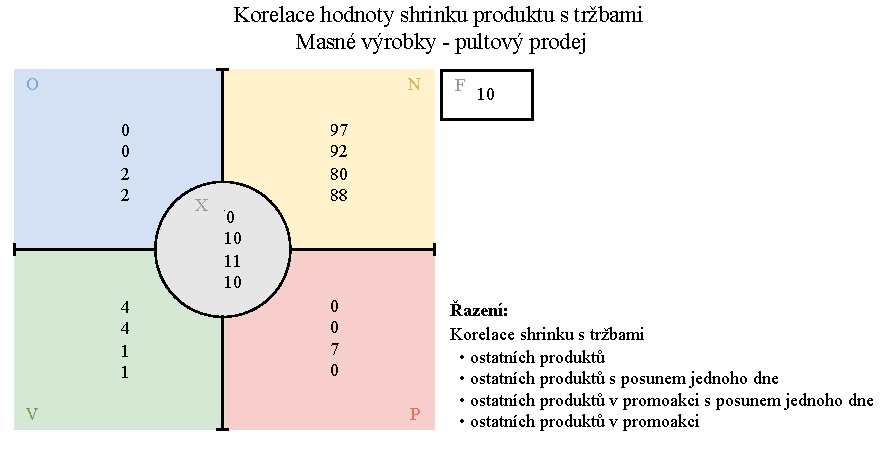
\includegraphics[width=\textwidth]{obrazky/kor_maso.pdf}
    \caption{Počet produktů z~kategorie Masné výrobky -- pultový prodej roztříděné pomocí korelační analýzy v~závislosti na různých ukazatelích.}
    \label{obr:kategCorrPorovnani}
\end{figure}

\begin{figure}[h!]
    \centering
    \captionsetup{justification=centering}
    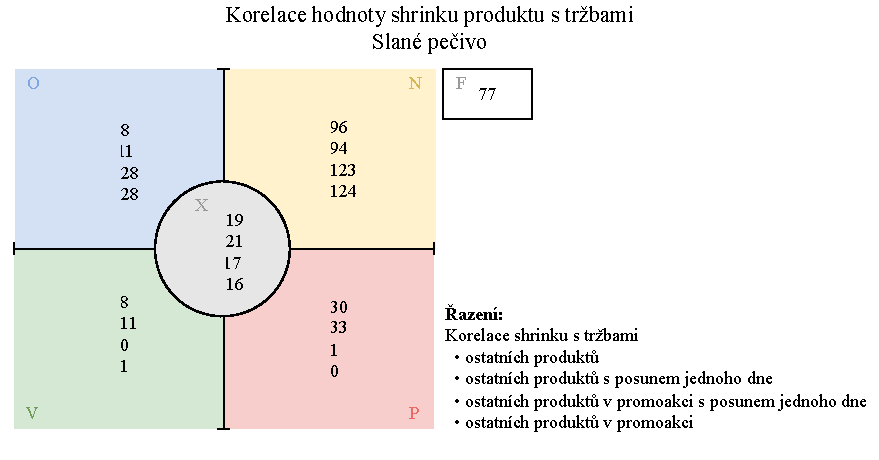
\includegraphics[width=\textwidth]{obrazky/kor_pec.pdf}
    \caption{Počet produktů z~kategorie Slané pečivo roztříděné pomocí korelační analýzy v~závislosti na různých ukazatelích.}
    \label{obr:kategCorrPorovnaniPec}
\end{figure}

\begin{figure}[h!]
    \centering
    \captionsetup{justification=centering}
    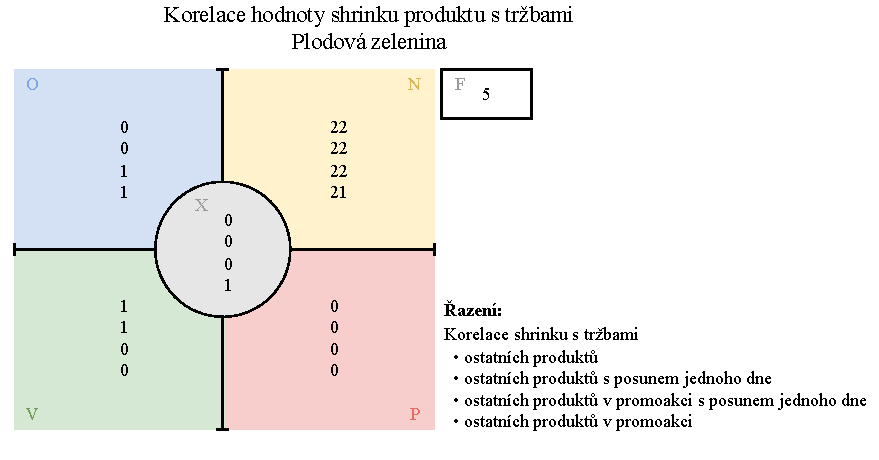
\includegraphics[width=\textwidth]{obrazky/kor_zel.pdf}
    \caption{Počet produktů z~kategorie Plodová zelenina roztříděné pomocí korelační analýzy v~závislosti na různých ukazatelích.}
    \label{obr:kategCorrPorovnaniZel}
\end{figure}

% \begin{table}[hbtp!]
%     \centering
%     \captionsetup{justification=centering}
%     \caption{Počet produktů v~kategoriích v~závislosti na různých ukazatelích. Kategorizace proběhla na základě Spearmanova korelačního koeficientu}
%     \begin{tabular}{l *{6}{r}}
%     \toprule
%     \multicolumn{1}{l}{} & \multicolumn{6}{c}{Korelace s~tržbami ostatních produktů} \\
%     \multicolumn{1}{l}{} & \multicolumn{2}{c}{Všechny prodeje} & \multicolumn{2}{c}{Prodeje v~promoakci}  & \multicolumn{2}{c}{Prodeje v~a po promoakci} \\
%     Kategorie & Stejný den & Další den & Stejný den & Další den & Stejný den & Další den \\
%     \midrule
%     \multicolumn{7}{c}{Masné výrobky -- pultový prodej} \\
%     \midrule
%     P           & 96   & 96   & 96   & 96   & 96   & 96   \\
%     O           & 1     & 1   & 2   & 2   & 2   & 2   \\
%     X           & 3     & 3   & 2   & 2   & 2   & 2   \\
%     Nevýzn.     & 11    & 11   & 11   & 11   & 11   & 11   \\
%     \midrule
%     \multicolumn{7}{c}{Slané pečivo} \\
%     \midrule
%     P           & 131   & 131   & 131   & 131   & 131   & 131   \\
%     O           & 9     & 13   & 24   & 24   & 24   & 24   \\
%     X           & 16    & 12   & 1    & 1    & 1    & 1    \\
%     Nevýzn.     & 90    & 90   & 90   & 90   & 90   & 90   \\
%     \bottomrule
%     \end{tabular}
%     \label{tab:kategCorrPorovnani}
% \end{table}

\textbf{Masné výrobky -- pultový prodej}

Shrink byl zaznamenaný u 111 produktů v~této kategorii úrovně 4. 88 produktů bylo klasifikováno jako kategorie N, deset jako kategorie X, dva jako kategorie O, jeden jako V. U zbylých deseti produktů nebyl koeficient korelace statisticky významný, a proto nejde u těchto produktů vyslovit hypotézu pro jejich zařazení. Korelace mezi hodnotou shrinku a promočními tržbami je na obr. \ref*{obr:corr:maso}.

\begin{figure}[h!]
    \centering
    \captionsetup{justification=centering}
    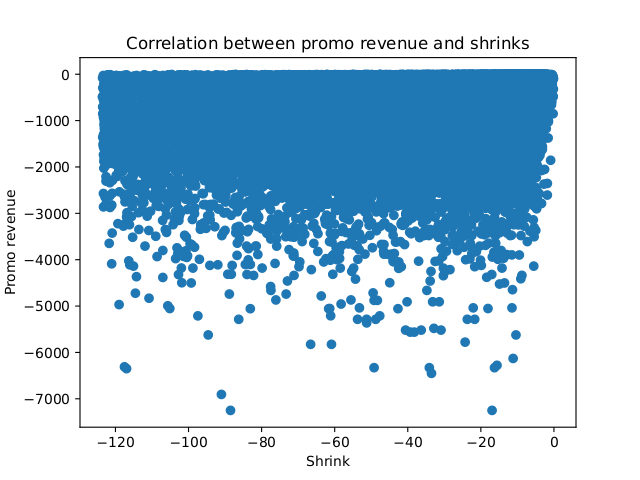
\includegraphics[width=.8\textwidth]{obrazky/grafy/categorization_charts/categorization_charts_L4_PROCMEAT.png}
    \caption{Závislost mezi tržbami produktu a tržbami ostatních produktů \\ v~kategorii během promoakce (Masné výrobky -- pultový prodej).}
    \label{obr:corr:maso}
\end{figure}

Produkty, které patří do kategorie O: Velikonoční klobása a Velikonoční šunka - jedná se zcela jistě o sezónní výrobky. Produkt, který byl označen jako výprodejový jsou Párky (Kuřecí striptýzky). Šest produktů z~kategorie nemělo během sledovaného období žádné evidované prodeje, všechny byly klasifikovány jako kategorie X, tedy hodnota koeficientu korelace neznamenala závislost. %{TODO: vyjmenovat i další produkty, které si způsobují samy, ale je to většina produktů a salámy, šunky, z~kategorie...} 

Dále jsem zkoumala podkategorie Masných výrobků. Porovnávala jsem prodeje v~rámci kategorií na šesté úrovni produktové hierarchie. V~podkategorii Salámy s~krátkou dobou spotřeby se kategorizace potvrdila. Pro kategorii, do níž patří sezónní výrobky - Netučné masné výrobky, nově z~této podkategorie byl jako kategorie O označen i produkt Kladenská pečeně.

Na obr. \ref*{obr:kor:vyslMASO} se nachází vizualizace získaných výsledků vygenerovaný pomocí Python knihovny \emph{plotly}. Při najetí na příslušné políčko (v~Jupyter Notebooku) se zobrazí údaje o produktu.

\begin{figure}[h!]
    \centering
    \captionsetup{justification=centering}
    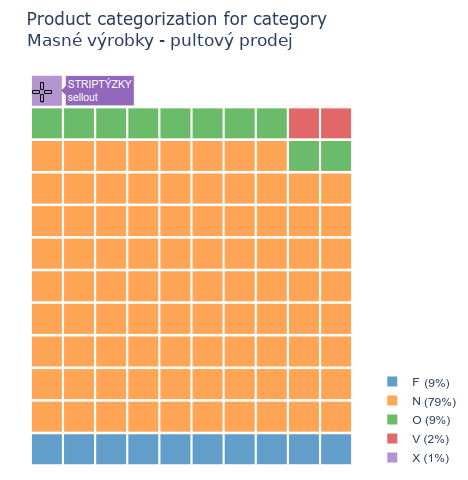
\includegraphics[width=.7\textwidth]{obrazky/zntb/vysledekMASO.png}
    \caption{Vizualizace výsledků rozdělení přiřazených kategorií \\ pro kategorii produktů Masné výrobky -- pultový prodej.}
    \label{obr:kor:vyslMASO}
\end{figure}


\textbf{Slané pečivo}

Shrink byl zaznamenaný u 246 produktů. 124 produktů bylo klasifikováno jako kategorie N, 16 jako kategorie X, 28 jako kategorie O, jeden jako P. Pro 77 produktů nebyl koeficient korelace statisticky významný. Jako produkt, který si způsobuje shrinky sám, byl označený obyčejný rohlík. Rohlík se tedy vyhazuje více čím vyšší jsou jeho vlastní tržby. Celkově patří tento produkt mezi ty s~největšími shrinky.

Produkty, které byly zařazeny do kategorie X, tj. takové, u kterých nebyl koeficient korelace dostatečně velký, byly produkty, které neměly během sledovaného období žádný prodej (promoční, či nepromoční).

% Produkty, které patří do kategorie O:
% pletýnka adélka, pletýnka malena, pletýnka sypaná mákem, pletýnka sypaná solí a km., bramborové pečivo s~cibulí, veka cupeko kb, rohlík grahamový aspec, rohlík pivní ora, rohlík staročeský, rohlík obilný mam, rohlík na strouh.karlova, rohl.n str.penam, houska mašek, houska raženka, bageta rust.poh., bageta s~grahamem, bageta chlebová, banketka cereální, dalamánek, kostka cereál malena, ciabatta mini natural, twistr se sýrem a špenatem, anglický rohlík, 

% \textbf{Sladké pečivo}

% % čokorolka, závin mák , skořicový vrut, donut bílý se sušnkami, závitek cereální nugátový, rohlík lístový s~ořech. náp, kobliha vanilková šiška, kobliha vanilková v~koš, kobliha s~jablky a skořicí, kobliha s~lísko.náp.a pol, koblih kapsa s~jablky, koláč wellartův, koláč tlač. vícezrnný, koláč šátek makový, koláč s~ovocnou nápl, koláček švestkový , koláček meruňkový , koláček borůvkový, koláč rohový tři náplně , koláč s~makovou náplní, koláč s~tvarohovo nápl, máslový koláč tvaroh, šátek kyn. tvarohová nápl, šáteček s~náplní višňovou , šáteček s~tvaroh.náplní, šátek makový, loupák o., loupák v., loupák m., závin tvaroh , závin kvásk. makový, bavorská hvězdice, makovka pletená mašek, croissant máslový

\textbf{Plodová zelenina}

Shrink byl zaznamenaný u 28 produktů v~této kategorii. 21 produktů bylo klasifikováno jako kategorie N, jeden produkt jako X a jeden jako O. U ostatních pěti produktů nebyl koeficient dostatečně významný. Produkt, který v~této kategorii neměl žádné prodeje byl pouze Lilek Bio, pro který koeficient korelace byl označen jako nevýznamný. Produkt, z~kategorie O, byla Cherry rajčata. Zatímco produkt z~ktegorie X, byl Paprika barevná Mix.

% product_id	warehouse_id	date_of_transaction	amount	cost_value	motive_type	weekday	quarter	warehouse_type	region	...	amount_share	whs_cost_value_share	promotion_type_1_id	promo	L1	L3	L4	L1_cost_value_share	L5	L6
% 0	24293174	644	2023-03-01	-0.47	-52.29	4	2	1	SM	Praha	...	0.1423	0.000005	NaN	no promo	SUPERFRESH	SF CM RED MEAT	RED MEAT	0.000060	MIX OF RED MEAT CHILLED	READY TO COOK RED MEAT CHILLED
% 1	26973548	644	2023-03-01	-2.00	-49.00	4	2	1	SM	Praha	...	0.0667	0.000005	NaN	no promo	SUPERFRESH	SF CM PROCESSED F&V	FRESH PROCESSED FV	0.000056	FRESH PROCESSED VEGETABLES	FRESH PROCESSED VEGETABLES SNACK
% 2	20428587	644	2023-03-01	-27.00	-44.55	4	2	1	SM	Praha	...	0.0076	0.000004	NaN	no promo	SUPERFRESH	SF CM BAKERY	SALTY PASTRY	0.000051	FRESH PASTRY BASIC	BUNS & KAISERKA
% 3	20480905	644	2023-03-01	-66.00	-106.26	4	2	1	SM	Praha	...	0.0082	0.000010	NaN	no promo	SUPERFRESH	SF CM BAKERY	SALTY PASTRY	0.000121	FRESH PASTRY BASIC	ROLL BASIC
% 4	23309074	644	2023-03-01	-1.00	-43.17	4	2	1	SM	Praha	...	0.1429	0.000004	NaN	no promo	SUPERFRESH	SF CM BAKERY	FRESH CONFECTIONARY	0.000049	FRESH CONFECTIONARY DESSERTS	FRESH DESSERTS
% 5 rows × 24 columns

% (811526, 24)
% product_id	promotion_type_1_id	promotion_date_from	promotion_date_to	warehouse_id	L3	L4	L5	L6	name
% 0	27630563	1	2023-02-22	2023-03-07	526	NaN	NaN	NaN	NaN	NaN
% 1	27653944	1	2023-02-22	2023-03-07	526	SF CM RED MEAT	RED MEAT	BEEF MEAT CHILLED	READY TO COOK RED MEAT CHILLED	BIO MASOVÉ KULIČKY 300G
% 2	27669921	1	2023-02-22	2023-03-07	526	FF CM CONVENIENCE	CHILLED PRODUCT SELF SERVICE	FRESH DELI PESTO & SAUCES SELF SERVICE	FRESH DELI VEGETARIAN SAUCES	NP VE BIO ORIENTAL TASTE 300G
% 3	27692653	1	2023-02-22	2023-03-07	526	FF CM CONVENIENCE	CHILLED PRODUCT SELF SERVICE	FRESH DELI PICKLED PRODUCTS SELF SERVICE	FRESH DELI PICKLED VEGETABLE	NP VE BIO KIMCHI NEPÁLIVÉ 350G
% 4	21817410	1	2023-02-22	2023-03-07	526	SF CM RED MEAT	RED MEAT	BEEF MEAT CHILLED	JOINT BEEF CHILLED	NP BIO HOV.ZADNÍ BK NA PEČENÍ
% (5539222, 10)
% product_id	warehouse_id	date_of_transaction	amount	cost_value	promotion_id	position_type	document_type_id	L3	L4	L5	L6	name	warehouse_type
% 0	20008963	820	2023-03-23	-1.0	-88.00	\N	2	150	NaN	NaN	NaN	NaN	NaN	HM
% 1	20013059	152	2023-03-14	-1.0	-25.38	\N	0	150	NaN	NaN	NaN	NaN	NaN	HM
% 2	20013059	152	2023-03-17	-4.0	-101.52	\N	0	150	NaN	NaN	NaN	NaN	NaN	HM
% 3	20013059	152	2023-03-19	-1.0	-25.38	\N	0	150	NaN	NaN	NaN	NaN	NaN	HM
% 4	20013059	152	2023-03-23	-1.0	-25.38	\N	0	150	NaN	NaN	NaN	NaN	NaN	HM
% (36575915, 14)

% ====================================================================================================================================================
% ====================================================================================================================================================
% ====================================================================================================================================================
% ====================================================================================================================================================
% MEAT
% % \begin{itemize}
% %     \itemsep0em 

% %     \item oboustranná: korelace je nenulová,
% %     \item jednostranná (menší než nula): korelace je záporná
% %     \item jednostranná (větší než nula): korelace je kladná
% % \end{itemize}

% %  MEAT PRODUCTS
% % Catgeorization:  correlation_with_other_products:
% % itself    96
% % False     11
% % None       3
% % other      1
% % Catgeorization:  correlation_with_other_products_past:
% % itself    96
% % False     11
% % None       4
% % Catgeorization:  correlation_with_other_products_promo:
% % itself    96
% % False     11
% % other      2
% % None       2
% % Catgeorization:  correlation_with_other_products_promo_past:
% % itself    96
% % False     11
% % other      2
% None       2

% Analyzing category: SALTY PASTRY of L4 category level.
% ======================================================
% Sizes of dataframes with obly the selected category: 
% Shape of df:  (104427, 22)
% Shape of df:  (8944, 10)
% Shape of df:  (480412, 14)
% Labeling promotions.
% 234020it [01:02, 3733.68it/s]
% Searching for duplicate records.
% 234020it [00:36, 6353.39it/s] 
% Count of rows to drop:  104772
% Shapes of dataframes: Sales:  (477631, 14) Promotions:  (8944, 10) Sales with promo:  (582403, 19) Sales with promo no duplicates:  (477631, 17)
% Calculating  spearman  correlation coefficient.
% Number of products in category:  246

% Products that had no sales during promotion:  223 products.
% Products that had no sales at all:  18 products.
% [22459466, 23194175, 26109718, 27344064, 22095022, 26627342, 21488931, 21976056, 21976124, 22045751, 26627328, 26778808, 25773071, 27735190, 27684436, 27740767, 27710340, 27740750]
% Catgeorization:  correlation_with_other_products:
% itself    131
% False      90
% None       16
% other       9

% Catgeorization:  correlation_with_other_products_past:
% itself    131
% False      90
% None       14
% other      11

% Catgeorization:  correlation_with_other_products_promo:
% itself    131
% False      90
% other      24
% None        1

% Catgeorization:  correlation_with_other_products_promo_past:
% itself    131
% False      90
% other      24
% None        1

% Analyzing category: FRUIT VEGETABLE of L4 category level.
% =========================================================
% Sizes of dataframes with obly the selected category: 
% Shape of df:  (34680, 22)
% Shape of df:  (5556, 10)
% Shape of df:  (179351, 14)
% Labeling promotions.
% 114262it [00:30, 3747.84it/s]
% Searching for duplicate records.
% 114262it [00:13, 8487.78it/s] 
% Count of rows to drop:  49439
% Shapes of dataframes: Sales:  (177703, 14) Promotions:  (5556, 10) Sales with promo:  (227142, 19) Sales with promo no duplicates:  (177703, 17)
% Calculating  spearman  correlation coefficient.
% Number of products in category:  28

% Products that had no sales during promotion:  16 products.
% [20444853, 20445836, 20698171, 26398969, 24363303, 20452094, 20445553, 21497513, 20446086, 27299395, 24228862, 24391078, 26977775, 23930742, 27227947, 27333501]
% Products that had no sales at all:  1 products.
% [27333501]
% Catgeorization:  correlation_with_other_products:
% itself    20
% False      8

% Catgeorization:  correlation_with_other_products_past:
% itself    20
% False      8

% Catgeorization:  correlation_with_other_products_promo:
% itself    20
% False      8

% Catgeorization:  correlation_with_other_products_promo_past:
% itself    20
% False      8

% Analyzing category: SWEET PASTRY of L4 category level.
% ======================================================
% Sizes of dataframes with obly the selected category: 
% Shape of df:  (48701, 22)
% Shape of df:  (16131, 10)
% Shape of df:  (634294, 14)
% Labeling promotions.
% 304122it [01:18, 3892.35it/s]
% Searching for duplicate records.
% 304122it [00:41, 7351.05it/s]
% Count of rows to drop:  24675
% Shapes of dataframes: Sales:  (632724, 14) Promotions:  (16131, 10) Sales with promo:  (657399, 19) Sales with promo no duplicates:  (632724, 17)
% Calculating  spearman  correlation coefficient.
% Number of products in category:  386

% Products that had no sales during promotion:  331 products.
% Products that had no sales at all:  10 products.
% [22055101, 27729915, 26159140, 26778860, 21976186, 26778846, 27738740, 27737170, 21976209, 27636015]
% Catgeorization:  correlation_with_other_products:
% False     197
% itself    155
% None       34

% Catgeorization:  correlation_with_other_products_past:
% False     197
% itself    155
% None       30
% other       4

% Catgeorization:  correlation_with_other_products_promo:
% False     197
% itself    155
% other      34

% Catgeorization:  correlation_with_other_products_promo_past:
% False     197
% itself    155
% other      34

% Analyzing category: RED MEAT of L4 category level.
% ==================================================
% Sizes of dataframes with obly the selected category: 
% Shape of df:  (17391, 22)
% Shape of df:  (29066, 10)
% Shape of df:  (332815, 14)
% Labeling promotions.
% 390190it [01:35, 4092.89it/s]
% Searching for duplicate records.
% 390190it [00:50, 7735.99it/s] 
% Count of rows to drop:  174298

% Products that had no sales during promotion:  65 products.
% [24293174, 24560115, 25720938, 24125499, 27725788, 24646864, 26040561, 26042824, 22840400, 26044910, 26566849, 26123615, 26130309, 26045061, 26045016, 27669778, 26045030, 26159881, 27166031, 22840387, 25881493, 26123677, 22257628, 26045115, 26124872, 26915975, 25960051, 26044811, 27712375, 25615036, 26872667, 26277202, 26770987, 26725192, 26044927, 26277226, 26177038, 27712399, 26044989, 27557235, 26770901, 27522660, 26643885, 26771007, 26771120, 27133279, 26157870, 26125275, 27743164, 26835846, 26871677, 26157733, 27102176, 26954905, 27260081, 27098868, 27103715, 27260265, 27738474, 27100912, 27425893, 27738481, 26566856, 27743157, 26771137]
% Products that had no sales at all:  17 products.
% [27725788, 26123615, 26130309, 26159881, 27166031, 26123677, 26124872, 26044989, 27133279, 26125275, 27743164, 26157733, 27098868, 27103715, 27738474, 27738481, 27743157]
% Catgeorization:  correlation_with_other_products:
% itself    96
% False     39
% None       3


% Catgeorization:  correlation_with_other_products_past:
% itself    96
% False     39
% None       3


% Catgeorization:  correlation_with_other_products_promo:
% itself    96
% False     39
% other      3


% Catgeorization:  correlation_with_other_products_promo_past:
% itself    96
% False     39
% other      3

% % https://docs.scipy.org/doc/scipy/reference/generated/scipy.stats.spearmanr.html
% % https://statistics.laerd.com/statistical-guides/spearmans-rank-order-correlation-statistical-guide-2.php There is no [monotonic] association between the two variables [in the population].






% Analyzing category: PROC. MEAT SERVICE of L4 category level.
% ============================================================
% Sizes of dataframes with obly the selected category: 
% Shape of df:  (303847, 22)
% Shape of df:  (70584, 10)
% Shape of df:  (555853, 14)
% Labeling promotions.
% 1679273it [08:33, 3270.31it/s]
% Searching for duplicate records.
% 1679273it [04:13, 6615.74it/s]
% Count of rows to drop:  1165224
% Shapes of dataframes: Sales:  (554305, 14) Promotions:  (70584, 10) Sales with promo:  (1719529, 19) Sales with promo no duplicates:  (554305, 17)
% Method:  pearson  after promo:  False
% Calculating  pearson  correlation coefficient.
% Number of products in category:  111

% Products that had no sales during promotion:  40 products.
% [20454081, 20454111, 25666854, 25961225, 26872896, 23180666, 20453978, 23373204, 24888967, 25478198, 25726787, 25961164, 26831718, 26831817, 27254783, 27571781, 27627761, 25726299, 25961140, 27150054, 25726046, 25726015, 25842371, 27571774, 20402082, 26835587, 25959000, 27722930, 27571798, 27736982, 27254486, 25726060, 27739174, 27737033, 27738504, 26835624, 27738733, 27611357, 25842579, 26831824]
% Products that had no sales at all:  6 products.
% [27722930, 27736982, 27739174, 27737033, 27738504, 27738733]
% Method:  pearson  after promo:  False
% Catgeorization:  correlation_with_other_products:
% itself    100
% False       9
% None        2


% Catgeorization:  correlation_with_other_products_past:
% itself    100
% False       9
% None        2


% Catgeorization:  correlation_with_other_products_promo:
% itself    100
% False       9
% other       1
% None        1


% Catgeorization:  correlation_with_other_products_promo_past:
% itself    100
% False       9
% other       1
% None        1


% Method:  spearman  after promo:  False
% Calculating  spearman  correlation coefficient.
% Number of products in category:  111
% Products that had no sales during promotion:  40 products.
% [20454081, 20454111, 25666854, 25961225, 26872896, 23180666, 20453978, 23373204, 24888967, 25478198, 25726787, 25961164, 26831718, 26831817, 27254783, 27571781, 27627761, 25726299, 25961140, 27150054, 25726046, 25726015, 25842371, 27571774, 20402082, 26835587, 25959000, 27722930, 27571798, 27736982, 27254486, 25726060, 27739174, 27737033, 27738504, 26835624, 27738733, 27611357, 25842579, 26831824]
% Products that had no sales at all:  6 products.
% [27722930, 27736982, 27739174, 27737033, 27738504, 27738733]
% Method:  spearman  after promo:  False
% Catgeorization:  correlation_with_other_products:
% itself    96
% False     11
% None       3
% other      1


% Catgeorization:  correlation_with_other_products_past:
% itself    96
% False     11
% None       3
% other      1


% Catgeorization:  correlation_with_other_products_promo:
% itself    96
% False     11
% other      2
% None       2


% Catgeorization:  correlation_with_other_products_promo_past:
% itself    96
% False     11
% other      2
% None       2


% Method:  pearson  after promo:  True
% Calculating  pearson  correlation coefficient.
% Number of products in category:  111
% Products that had no sales during promotion:  32 products.
% [26872896, 24888967, 25478198, 25726787, 25961164, 26831718, 26831817, 27254783, 27571781, 27627761, 25726299, 25961140, 27150054, 25726046, 25726015, 27571774, 20402082, 26835587, 25959000, 27722930, 27571798, 27736982, 27254486, 25726060, 27739174, 27737033, 27738504, 26835624, 27738733, 27611357, 25842579, 26831824]
% Products that had no sales at all:  6 products.
% [27722930, 27736982, 27739174, 27737033, 27738504, 27738733]
% Method:  pearson  after promo:  True
% Catgeorization:  correlation_with_other_products:
% itself    100
% False       9
% None        2


% Catgeorization:  correlation_with_other_products_past:
% itself    100
% False       9
% None        2


% Catgeorization:  correlation_with_other_products_promo:
% itself    100
% False       9
% other       1
% None        1


% Catgeorization:  correlation_with_other_products_promo_past:
% itself    100
% False       9
% other       1
% None        1


% Method:  spearman  after promo:  True
% Calculating  spearman  correlation coefficient.
% Number of products in category:  111
% Products that had no sales during promotion:  32 products.
% [26872896, 24888967, 25478198, 25726787, 25961164, 26831718, 26831817, 27254783, 27571781, 27627761, 25726299, 25961140, 27150054, 25726046, 25726015, 27571774, 20402082, 26835587, 25959000, 27722930, 27571798, 27736982, 27254486, 25726060, 27739174, 27737033, 27738504, 26835624, 27738733, 27611357, 25842579, 26831824]
% Products that had no sales at all:  6 products.
% [27722930, 27736982, 27739174, 27737033, 27738504, 27738733]
% Method:  spearman  after promo:  True
% Catgeorization:  correlation_with_other_products:
% itself    96
% False     11
% None       4


% Catgeorization:  correlation_with_other_products_past:
% itself    96
% False     11
% None       4


% Catgeorization:  correlation_with_other_products_promo:
% itself    96
% False     11
% other      2
% None       2


% Catgeorization:  correlation_with_other_products_promo_past:
% itself    96
% False     11
% other      2
% None       2


% Analyzing category: SALTY PASTRY of L4 category level.
% ======================================================
% Sizes of dataframes with obly the selected category: 
% Shape of df:  (104427, 22)
% Shape of df:  (8944, 10)
% Shape of df:  (480412, 14)
% Labeling promotions.
% 234020it [01:11, 3260.33it/s]
% Searching for duplicate records.
% 234020it [00:30, 7668.35it/s] 
% Count of rows to drop:  104772
% Shapes of dataframes: Sales:  (477631, 14) Promotions:  (8944, 10) Sales with promo:  (582403, 19) Sales with promo no duplicates:  (477631, 17)
% Method:  pearson  after promo:  False
% Calculating  pearson  correlation coefficient.
% Number of products in category:  246
% Products that had no sales during promotion:  227 products.
% [20428587, 20480905, 21852039, 23472266, 25467697, 27422731, 27442449, 27456934, 27516850, 27516867, 27544884, 27544907, 27544952, 27544983, 27578025, 27609699, 25672985, 26782034, 27544914, 27544938, 23472259, 27123195, 27544877, 27544891, 27603581, 25310863, 26576442, 26627373, 27123201, 27274750, 27574270, 22459466, 23194175, 23549074, 25895667, 26109718, 26737430, 26737461, 26737478, 27266038, 27269244, 27344064, 27603598, 27619810, 22095022, 26627342, 27638019, 20783808, 21488931, 21976056, 21976124, 22045751, 26627328, 26709468, 27442760, 27312759, 26737539, 26778808, 21471971, 24587136, 27544969, 25318074, 25322194, 25892369, 26960975, 25512700, 23319905, 25673005, 23635739, 25516234, 26359205, 25012200, 25175639, 25431483, 25430783, 25430837, 25430820, 25773071, 27075234, 27075227, 25629620, 26571362, 26571324, 26571331, 27601532, 26786698, 27710418, 22941404, 25504422, 27034071, 26975085, 27449943, 25548761, 25663075, 27195000, 24744881, 27641569, 26445540, 27201930, 22957733, 27374993, 22962294, 25426496, 25426502, 25254792, 27610640, 25506242, 26546117, 27610664, 27735190, 25507294, 25507256, 25506297, 25506303, 22993847, 22993885, 25504439, 25504460, 25571608, 25431599, 27329290, 21482922, 24174381, 25390261, 25390254, 25390643, 25394368, 24328579, 25665864, 24644167, 27329269, 25594836, 22933904, 22933973, 27619513, 27384039, 27384053, 25393422, 25891966, 27134641, 27134634, 23549067, 27152706, 25665802, 25605327, 26787008, 25630602, 26035062, 27455630, 25504446, 27620175, 25571615, 25571660, 27134658, 27134665, 27134689, 24323611, 25498554, 25630596, 25630619, 27619520, 26802046, 27134719, 26975740, 27603611, 25513318, 27282670, 27696729, 27466261, 22993892, 22662200, 25630466, 22019943, 27712306, 27684436, 27278116, 26381350, 26885506, 27307656, 26389400, 27329139, 22516657, 27329184, 27329115, 27032404, 27215937, 26386973, 27453179, 27715444, 25756999, 27128473, 26347394, 27136768, 25661224, 24277365, 25048698, 26434582, 27152492, 27715451, 23478992, 26975078, 26391175, 26802060, 25326185, 26381459, 26576848, 24644143, 25605273, 25066159, 25630657, 26581798, 27574225, 26975689, 27620182, 26381381, 24704427, 26975764, 24644150, 22126221, 25504491, 27710432, 27740767, 27710340, 26502755, 27312827, 27740750, 26579221]
% Products that had no sales at all:  18 products.
% [22459466, 23194175, 26109718, 27344064, 22095022, 26627342, 21488931, 21976056, 21976124, 22045751, 26627328, 26778808, 25773071, 27735190, 27684436, 27740767, 27710340, 27740750]
% Method:  pearson  after promo:  False
% Catgeorization:  correlation_with_other_products:
% itself    130
% False     100
% None       13
% other       3


% Catgeorization:  correlation_with_other_products_past:
% itself    130
% False     100
% None       11
% other       5


% Catgeorization:  correlation_with_other_products_promo:
% itself    130
% False     100
% other      16


% Catgeorization:  correlation_with_other_products_promo_past:
% itself    130
% False     100
% other      16


% Method:  spearman  after promo:  False
% Calculating  spearman  correlation coefficient.
% Number of products in category:  246
% Products that had no sales during promotion:  227 products.
% [20428587, 20480905, 21852039, 23472266, 25467697, 27422731, 27442449, 27456934, 27516850, 27516867, 27544884, 27544907, 27544952, 27544983, 27578025, 27609699, 25672985, 26782034, 27544914, 27544938, 23472259, 27123195, 27544877, 27544891, 27603581, 25310863, 26576442, 26627373, 27123201, 27274750, 27574270, 22459466, 23194175, 23549074, 25895667, 26109718, 26737430, 26737461, 26737478, 27266038, 27269244, 27344064, 27603598, 27619810, 22095022, 26627342, 27638019, 20783808, 21488931, 21976056, 21976124, 22045751, 26627328, 26709468, 27442760, 27312759, 26737539, 26778808, 21471971, 24587136, 27544969, 25318074, 25322194, 25892369, 26960975, 25512700, 23319905, 25673005, 23635739, 25516234, 26359205, 25012200, 25175639, 25431483, 25430783, 25430837, 25430820, 25773071, 27075234, 27075227, 25629620, 26571362, 26571324, 26571331, 27601532, 26786698, 27710418, 22941404, 25504422, 27034071, 26975085, 27449943, 25548761, 25663075, 27195000, 24744881, 27641569, 26445540, 27201930, 22957733, 27374993, 22962294, 25426496, 25426502, 25254792, 27610640, 25506242, 26546117, 27610664, 27735190, 25507294, 25507256, 25506297, 25506303, 22993847, 22993885, 25504439, 25504460, 25571608, 25431599, 27329290, 21482922, 24174381, 25390261, 25390254, 25390643, 25394368, 24328579, 25665864, 24644167, 27329269, 25594836, 22933904, 22933973, 27619513, 27384039, 27384053, 25393422, 25891966, 27134641, 27134634, 23549067, 27152706, 25665802, 25605327, 26787008, 25630602, 26035062, 27455630, 25504446, 27620175, 25571615, 25571660, 27134658, 27134665, 27134689, 24323611, 25498554, 25630596, 25630619, 27619520, 26802046, 27134719, 26975740, 27603611, 25513318, 27282670, 27696729, 27466261, 22993892, 22662200, 25630466, 22019943, 27712306, 27684436, 27278116, 26381350, 26885506, 27307656, 26389400, 27329139, 22516657, 27329184, 27329115, 27032404, 27215937, 26386973, 27453179, 27715444, 25756999, 27128473, 26347394, 27136768, 25661224, 24277365, 25048698, 26434582, 27152492, 27715451, 23478992, 26975078, 26391175, 26802060, 25326185, 26381459, 26576848, 24644143, 25605273, 25066159, 25630657, 26581798, 27574225, 26975689, 27620182, 26381381, 24704427, 26975764, 24644150, 22126221, 25504491, 27710432, 27740767, 27710340, 26502755, 27312827, 27740750, 26579221]
% Products that had no sales at all:  18 products.
% [22459466, 23194175, 26109718, 27344064, 22095022, 26627342, 21488931, 21976056, 21976124, 22045751, 26627328, 26778808, 25773071, 27735190, 27684436, 27740767, 27710340, 27740750]
% Method:  spearman  after promo:  False
% Catgeorization:  correlation_with_other_products:
% itself    131
% False      90
% None       16
% other       9


% Catgeorization:  correlation_with_other_products_past:
% itself    131
% False      90
% other      13
% None       12


% Catgeorization:  correlation_with_other_products_promo:
% itself    131
% False      90
% other      24
% None        1


% Catgeorization:  correlation_with_other_products_promo_past:
% itself    131
% False      90
% other      24
% None        1


% Method:  pearson  after promo:  True
% Calculating  pearson  correlation coefficient.
% Number of products in category:  246
% 246it [01:23,  2.93it/s]
% Products that had no sales during promotion:  223 products.
% [20428587, 20480905, 21852039, 23472266, 25467697, 27442449, 27456934, 27516850, 27516867, 27544884, 27544907, 27544952, 27544983, 27578025, 27609699, 25672985, 26782034, 27544914, 27544938, 23472259, 27123195, 27544877, 27544891, 25310863, 26576442, 26627373, 27123201, 27274750, 27574270, 22459466, 23194175, 23549074, 25895667, 26109718, 26737430, 26737461, 26737478, 27266038, 27269244, 27344064, 27619810, 22095022, 26627342, 27638019, 20783808, 21488931, 21976056, 21976124, 22045751, 26627328, 26709468, 27442760, 27312759, 26737539, 26778808, 21471971, 24587136, 27544969, 25318074, 25322194, 25892369, 25512700, 23319905, 25673005, 23635739, 25516234, 26359205, 25012200, 25175639, 25431483, 25430783, 25430837, 25430820, 25773071, 27075234, 27075227, 25629620, 26571362, 26571324, 26571331, 27601532, 26786698, 27710418, 22941404, 25504422, 27034071, 26975085, 27449943, 25548761, 25663075, 27195000, 24744881, 27641569, 26445540, 27201930, 22957733, 27374993, 22962294, 25426496, 25426502, 25254792, 27610640, 25506242, 26546117, 27610664, 27735190, 25507294, 25507256, 25506297, 25506303, 22993847, 22993885, 25504439, 25504460, 25571608, 25431599, 27329290, 21482922, 24174381, 25390261, 25390254, 25390643, 25394368, 24328579, 25665864, 24644167, 27329269, 25594836, 22933904, 22933973, 27619513, 27384039, 27384053, 25393422, 25891966, 27134641, 27134634, 23549067, 27152706, 25665802, 25605327, 26787008, 25630602, 26035062, 27455630, 25504446, 27620175, 25571615, 25571660, 27134658, 27134665, 27134689, 24323611, 25498554, 25630596, 25630619, 27619520, 26802046, 27134719, 26975740, 27603611, 25513318, 27282670, 27696729, 27466261, 22993892, 22662200, 25630466, 22019943, 27712306, 27684436, 27278116, 26381350, 26885506, 27307656, 26389400, 27329139, 22516657, 27329184, 27329115, 27032404, 27215937, 26386973, 27453179, 27715444, 25756999, 27128473, 26347394, 27136768, 25661224, 24277365, 25048698, 26434582, 27152492, 27715451, 23478992, 26975078, 26391175, 26802060, 25326185, 26381459, 26576848, 24644143, 25605273, 25066159, 25630657, 26581798, 27574225, 26975689, 27620182, 26381381, 24704427, 26975764, 24644150, 22126221, 25504491, 27710432, 27740767, 27710340, 26502755, 27312827, 27740750, 26579221]
% Products that had no sales at all:  18 products.
% [22459466, 23194175, 26109718, 27344064, 22095022, 26627342, 21488931, 21976056, 21976124, 22045751, 26627328, 26778808, 25773071, 27735190, 27684436, 27740767, 27710340, 27740750]
% Method:  pearson  after promo:  True
% Catgeorization:  correlation_with_other_products:
% itself    130
% False     100
% None       14
% other       2


% Catgeorization:  correlation_with_other_products_past:
% itself    130
% False     100
% None       13
% other       3


% Catgeorization:  correlation_with_other_products_promo:
% itself    130
% False     100
% other      16


% Catgeorization:  correlation_with_other_products_promo_past:
% itself    130
% False     100
% other      16


% Method:  spearman  after promo:  True
% Products that had no sales during promotion:  223 products.
% [20428587, 20480905, 21852039, 23472266, 25467697, 27442449, 27456934, 27516850, 27516867, 27544884, 27544907, 27544952, 27544983, 27578025, 27609699, 25672985, 26782034, 27544914, 27544938, 23472259, 27123195, 27544877, 27544891, 25310863, 26576442, 26627373, 27123201, 27274750, 27574270, 22459466, 23194175, 23549074, 25895667, 26109718, 26737430, 26737461, 26737478, 27266038, 27269244, 27344064, 27619810, 22095022, 26627342, 27638019, 20783808, 21488931, 21976056, 21976124, 22045751, 26627328, 26709468, 27442760, 27312759, 26737539, 26778808, 21471971, 24587136, 27544969, 25318074, 25322194, 25892369, 25512700, 23319905, 25673005, 23635739, 25516234, 26359205, 25012200, 25175639, 25431483, 25430783, 25430837, 25430820, 25773071, 27075234, 27075227, 25629620, 26571362, 26571324, 26571331, 27601532, 26786698, 27710418, 22941404, 25504422, 27034071, 26975085, 27449943, 25548761, 25663075, 27195000, 24744881, 27641569, 26445540, 27201930, 22957733, 27374993, 22962294, 25426496, 25426502, 25254792, 27610640, 25506242, 26546117, 27610664, 27735190, 25507294, 25507256, 25506297, 25506303, 22993847, 22993885, 25504439, 25504460, 25571608, 25431599, 27329290, 21482922, 24174381, 25390261, 25390254, 25390643, 25394368, 24328579, 25665864, 24644167, 27329269, 25594836, 22933904, 22933973, 27619513, 27384039, 27384053, 25393422, 25891966, 27134641, 27134634, 23549067, 27152706, 25665802, 25605327, 26787008, 25630602, 26035062, 27455630, 25504446, 27620175, 25571615, 25571660, 27134658, 27134665, 27134689, 24323611, 25498554, 25630596, 25630619, 27619520, 26802046, 27134719, 26975740, 27603611, 25513318, 27282670, 27696729, 27466261, 22993892, 22662200, 25630466, 22019943, 27712306, 27684436, 27278116, 26381350, 26885506, 27307656, 26389400, 27329139, 22516657, 27329184, 27329115, 27032404, 27215937, 26386973, 27453179, 27715444, 25756999, 27128473, 26347394, 27136768, 25661224, 24277365, 25048698, 26434582, 27152492, 27715451, 23478992, 26975078, 26391175, 26802060, 25326185, 26381459, 26576848, 24644143, 25605273, 25066159, 25630657, 26581798, 27574225, 26975689, 27620182, 26381381, 24704427, 26975764, 24644150, 22126221, 25504491, 27710432, 27740767, 27710340, 26502755, 27312827, 27740750, 26579221]
% Products that had no sales at all:  18 products.
% [22459466, 23194175, 26109718, 27344064, 22095022, 26627342, 21488931, 21976056, 21976124, 22045751, 26627328, 26778808, 25773071, 27735190, 27684436, 27740767, 27710340, 27740750]
% Method:  spearman  after promo:  True
% Catgeorization:  correlation_with_other_products:
% itself    131
% False      90
% None       16
% other       9


% Catgeorization:  correlation_with_other_products_past:
% itself    131
% False      90
% None       14
% other      11


% Catgeorization:  correlation_with_other_products_promo:
% itself    131
% False      90
% other      24
% None        1


% Catgeorization:  correlation_with_other_products_promo_past:
% itself    131
% False      90
% other      24
% None        1


% ./categorization_charts/categorization_charts_L4_SALTY PASTRY.pdf
% Analyzing category: FRUIT VEGETABLE of L4 category level.
% =========================================================
% Sizes of dataframes with obly the selected category: 
% Shape of df:  (34680, 22)
% Shape of df:  (5556, 10)
% Shape of df:  (179351, 14)
% Labeling promotions.
% 114262it [00:29, 3873.93it/s]
% Searching for duplicate records.
% 114262it [00:14, 8118.47it/s]
% Count of rows to drop:  49439
% Shapes of dataframes: Sales:  (177703, 14) Promotions:  (5556, 10) Sales with promo:  (227142, 19) Sales with promo no duplicates:  (177703, 17)
% Method:  pearson  after promo:  False
% Calculating  pearson  correlation coefficient.
% Number of products in category:  28

% Products that had no sales during promotion:  17 products.
% [20444853, 20445836, 20698171, 26398969, 24363303, 20452094, 20445553, 21497513, 20446086, 27299395, 24228862, 24391078, 27186244, 26977775, 23930742, 27227947, 27333501]
% Products that had no sales at all:  1 products.
% [27333501]
% Method:  pearson  after promo:  False
% Catgeorization:  correlation_with_other_products:
% itself    23
% False      5


% Catgeorization:  correlation_with_other_products_past:
% itself    23
% False      5


% Catgeorization:  correlation_with_other_products_promo:
% itself    23
% False      5


% Catgeorization:  correlation_with_other_products_promo_past:
% itself    23
% False      5


% Method:  spearman  after promo:  False
% Calculating  spearman  correlation coefficient.
% Number of products in category:  28

% Products that had no sales during promotion:  17 products.
% [20444853, 20445836, 20698171, 26398969, 24363303, 20452094, 20445553, 21497513, 20446086, 27299395, 24228862, 24391078, 27186244, 26977775, 23930742, 27227947, 27333501]
% Products that had no sales at all:  1 products.
% [27333501]
% Method:  spearman  after promo:  False
% Catgeorization:  correlation_with_other_products:
% itself    20
% False      8


% Catgeorization:  correlation_with_other_products_past:
% itself    20
% False      8


% Catgeorization:  correlation_with_other_products_promo:
% itself    20
% False      8


% Catgeorization:  correlation_with_other_products_promo_past:
% itself    20
% False      8


% Method:  pearson  after promo:  True
% Calculating  pearson  correlation coefficient.
% Number of products in category:  28

% Products that had no sales during promotion:  16 products.
% [20444853, 20445836, 20698171, 26398969, 24363303, 20452094, 20445553, 21497513, 20446086, 27299395, 24228862, 24391078, 26977775, 23930742, 27227947, 27333501]
% Products that had no sales at all:  1 products.
% [27333501]
% Method:  pearson  after promo:  True
% Catgeorization:  correlation_with_other_products:
% itself    23
% False      5


% Catgeorization:  correlation_with_other_products_past:
% itself    23
% False      5


% Catgeorization:  correlation_with_other_products_promo:
% itself    23
% False      5


% Catgeorization:  correlation_with_other_products_promo_past:
% itself    23
% False      5


% Method:  spearman  after promo:  True
% Calculating  spearman  correlation coefficient.
% Number of products in category:  28

% Products that had no sales during promotion:  16 products.
% [20444853, 20445836, 20698171, 26398969, 24363303, 20452094, 20445553, 21497513, 20446086, 27299395, 24228862, 24391078, 26977775, 23930742, 27227947, 27333501]
% Products that had no sales at all:  1 products.
% [27333501]
% Method:  spearman  after promo:  True
% Catgeorization:  correlation_with_other_products:
% itself    20
% False      8


% Catgeorization:  correlation_with_other_products_past:
% itself    20
% False      8


% Catgeorization:  correlation_with_other_products_promo:
% itself    20
% False      8


% Catgeorization:  correlation_with_other_products_promo_past:
% itself    20
% False      8


% ./categorization_charts/categorization_charts_L4_FRUIT VEGETABLE.pdf
% Analyzing category: SWEET PASTRY of L4 category level.
% ======================================================
% Sizes of dataframes with obly the selected category: 
% Shape of df:  (48701, 22)
% Shape of df:  (16131, 10)
% Shape of df:  (634294, 14)
% Labeling promotions.
% 304122it [01:10, 4326.14it/s]
% Searching for duplicate records.
% 304122it [00:43, 6952.49it/s]
% Count of rows to drop:  24675
% Shapes of dataframes: Sales:  (632724, 14) Promotions:  (16131, 10) Sales with promo:  (657399, 19) Sales with promo no duplicates:  (632724, 17)
% Method:  pearson  after promo:  False
% Calculating  pearson  correlation coefficient.
% Number of products in category:  386

% Products that had no sales during promotion:  339 products.

% Products that had no sales at all:  10 products.
% [22055101, 27729915, 26159140, 26778860, 21976186, 26778846, 27738740, 27737170, 21976209, 27636015]
% Method:  pearson  after promo:  False
% Catgeorization:  correlation_with_other_products:
% False     228
% itself    143
% None       15


% Catgeorization:  correlation_with_other_products_past:
% False     228
% itself    143
% None       15


% Catgeorization:  correlation_with_other_products_promo:
% False     228
% itself    143
% other      15


% Catgeorization:  correlation_with_other_products_promo_past:
% False     228
% itself    143
% other      15


% Method:  spearman  after promo:  False
% Calculating  spearman  correlation coefficient.
% Number of products in category:  386

% Products that had no sales at all:  10 products.
% [22055101, 27729915, 26159140, 26778860, 21976186, 26778846, 27738740, 27737170, 21976209, 27636015]
% Method:  spearman  after promo:  False
% Catgeorization:  correlation_with_other_products:
% False     197
% itself    155
% None       34


% Catgeorization:  correlation_with_other_products_past:
% False     197
% itself    155
% None       31
% other       3


% Catgeorization:  correlation_with_other_products_promo:
% False     197
% itself    155
% other      34


% Catgeorization:  correlation_with_other_products_promo_past:
% False     197
% itself    155
% other      34


% Method:  pearson  after promo:  True
% Calculating  pearson  correlation coefficient.
% Number of products in category:  386

% Products that had no sales at all:  10 products.
% [22055101, 27729915, 26159140, 26778860, 21976186, 26778846, 27738740, 27737170, 21976209, 27636015]
% Method:  pearson  after promo:  True
% Catgeorization:  correlation_with_other_products:
% False     228
% itself    143
% None       15


% Catgeorization:  correlation_with_other_products_past:
% False     228
% itself    143
% None       15


% Catgeorization:  correlation_with_other_products_promo:
% False     228
% itself    143
% other      15


% Catgeorization:  correlation_with_other_products_promo_past:
% False     228
% itself    143
% other      15


% Method:  spearman  after promo:  True
% Calculating  spearman  correlation coefficient.
% Number of products in category:  386
% Method:  spearman  after promo:  True
% Catgeorization:  correlation_with_other_products:
% False     197
% itself    155
% None       34


% Catgeorization:  correlation_with_other_products_past:
% False     197
% itself    155
% None       30
% other       4


% Catgeorization:  correlation_with_other_products_promo:
% False     197
% itself    155
% other      34


% Catgeorization:  correlation_with_other_products_promo_past:
% False     197
% itself    155
% other      34


% ./categorization_charts/categorization_charts_L4_SWEET PASTRY.pdf
% Analyzing category: RED MEAT of L4 category level.
% ==================================================
% Sizes of dataframes with obly the selected category: 
% Shape of df:  (17391, 22)
% Shape of df:  (29066, 10)
% Shape of df:  (332815, 14)
% Labeling promotions.
% 390190it [01:53, 3428.34it/s]
% Searching for duplicate records.
% 390190it [00:53, 7325.67it/s] 
% Count of rows to drop:  174298
% Shapes of dataframes: Sales:  (331211, 14) Promotions:  (29066, 10) Sales with promo:  (505509, 19) Sales with promo no duplicates:  (331211, 17)
% Method:  pearson  after promo:  False
% Calculating  pearson  correlation coefficient.
% Number of products in category:  138
% Products that had no sales at all:  17 products.
% [27725788, 26123615, 26130309, 26159881, 27166031, 26123677, 26124872, 26044989, 27133279, 26125275, 27743164, 26157733, 27098868, 27103715, 27738474, 27738481, 27743157]
% Method:  pearson  after promo:  False
% Catgeorization:  correlation_with_other_products:
% itself    98
% False     36
% None       4


% Catgeorization:  correlation_with_other_products_past:
% itself    98
% False     36
% None       4


% Catgeorization:  correlation_with_other_products_promo:
% itself    98
% False     36
% other      3
% None       1


% Catgeorization:  correlation_with_other_products_promo_past:
% itself    98
% False     36
% other      3
% None       1


% Method:  spearman  after promo:  False
% Calculating  spearman  correlation coefficient.
% Number of products in category:  138
% Method:  spearman  after promo:  False
% Catgeorization:  correlation_with_other_products:
% itself    96
% False     39
% None       3


% Catgeorization:  correlation_with_other_products_past:
% itself    96
% False     39
% None       3


% Catgeorization:  correlation_with_other_products_promo:
% itself    96
% False     39
% other      3


% Catgeorization:  correlation_with_other_products_promo_past:
% itself    96
% False     39
% other      3


% Method:  pearson  after promo:  True
% Calculating  pearson  correlation coefficient.
% Number of products in category:  138
% Catgeorization:  correlation_with_other_products:
% itself    98
% False     36
% None       4


% Catgeorization:  correlation_with_other_products_past:
% itself    98
% False     36
% None       4


% Catgeorization:  correlation_with_other_products_promo:
% itself    98
% False     36
% other      3
% None       1


% Catgeorization:  correlation_with_other_products_promo_past:
% itself    98
% False     36
% other      3
% None       1


% Method:  spearman  after promo:  True
% Calculating  spearman  correlation coefficient.
% Number of products in category:  138
% Method:  spearman  after promo:  True
% Catgeorization:  correlation_with_other_products:
% itself    96
% False     39
% None       3


% Catgeorization:  correlation_with_other_products_past:
% itself    96
% False     39
% None       3


% Catgeorization:  correlation_with_other_products_promo:
% itself    96
% False     39
% other      3


% Catgeorization:  correlation_with_other_products_promo_past:
% itself    96
% False     39
% other      3


% ./categorization_charts/categorization_charts_L4_RED MEAT.pdf
% Analyzing category: BREAD of L4 category level.
% ===============================================
% Sizes of dataframes with obly the selected category: 
% Shape of df:  (28750, 22)
% Shape of df:  (3463, 10)
% Shape of df:  (394320, 14)
% Labeling promotions.
% 90421it [00:27, 3314.86it/s]
% Searching for duplicate records.
% 90421it [00:15, 5783.06it/s]
% Count of rows to drop:  43979
% Products that had no sales at all:  86 products.
% [27062715, 26778785, 27711200, 27529997, 27722800, 27710319, 25586015, 25597301, 25586855, 25586657, 25586688, 27131466, 27259528, 25586053, 25586725, 25589535, 27727461, 25586695, 25589627, 25589832, 25586848, 27247105, 27247129, 25586763, 25586114, 25586107, 25586701, 25586664, 25586862, 25586879, 25586060, 25586596, 25586909, 25586916, 25586602, 25586619, 25665147, 25586138, 25586503, 25586091, 25586084, 25586077, 25586411, 25586404, 27643822, 26804934, 27710333, 27643839, 25585988, 25586787, 26804903, 26316208, 25589924, 25589542, 25586893, 25589528, 25715651, 25589856, 27625378, 27711286, 26316451, 27711293, 25589580, 27745670, 25589825, 25589870, 27750216, 27745663, 25586046, 25665130, 27746509, 27754238, 25586022, 26410692, 27735039, 25586718, 25586794, 25586121, 27750193, 25586039, 25589672, 25586671, 25589818, 25586770, 27758731, 27747117]
% Method:  pearson  after promo:  False
% Catgeorization:  correlation_with_other_products:
% False     255
% itself    143
% None       21


% Catgeorization:  correlation_with_other_products_past:
% False     255
% itself    143
% None       20
% other       1


% Catgeorization:  correlation_with_other_products_promo:
% False     255
% itself    143
% other      13
% None        8


% Catgeorization:  correlation_with_other_products_promo_past:
% False     255
% itself    143
% other      13
% None        8


% Method:  spearman  after promo:  False
% Calculating  spearman  correlation coefficient.
% Number of products in category:  419
% Method:  spearman  after promo:  False
% Catgeorization:  correlation_with_other_products:
% False     225
% itself    157
% None       29
% other       8


% Catgeorization:  correlation_with_other_products_past:
% False     225
% itself    157
% None       26
% other      11


% Catgeorization:  correlation_with_other_products_promo:
% False     225
% itself    157
% other      24
% None       13


% Catgeorization:  correlation_with_other_products_promo_past:
% False     225
% itself    157
% other      23
% None       14


% Method:  pearson  after promo:  True
% Calculating  pearson  correlation coefficient.
% Number of products in category:  419
% Method:  pearson  after promo:  True
% Catgeorization:  correlation_with_other_products:
% False     255
% itself    143
% None       21


% Catgeorization:  correlation_with_other_products_past:
% False     255
% itself    143
% None       21


% Catgeorization:  correlation_with_other_products_promo:
% False     255
% itself    143
% other      13
% None        8


% Catgeorization:  correlation_with_other_products_promo_past:
% False     255
% itself    143
% other      13
% None        8


% Method:  spearman  after promo:  True
% Calculating  spearman  correlation coefficient.
% Number of products in category:  419
% Method:  spearman  after promo:  True
% Catgeorization:  correlation_with_other_products:
% False     225
% itself    157
% None       27
% other      10


% Catgeorization:  correlation_with_other_products_past:
% False     225
% itself    157
% None       26
% other      11


% Catgeorization:  correlation_with_other_products_promo:
% False     225
% itself    157
% other      24
% None       13


% Catgeorization:  correlation_with_other_products_promo_past:
% False     225
% itself    157
% other      23
% None       14


% ./categorization_charts/categorization_charts_L4_BREAD.pdf
% Analyzing category: CITRUSES of L4 category level.
% ==================================================
% Sizes of dataframes with obly the selected category: 
% Shape of df:  (26646, 22)
% Shape of df:  (6364, 10)
% Shape of df:  (88119, 14)
% Labeling promotions.
% 153368it [00:41, 3657.83it/s]
% Searching for duplicate records.
% 153368it [00:20, 7608.09it/s]
% Count of rows to drop:  79062
% Shapes of dataframes: Sales:  (86946, 14) Promotions:  (6364, 10) Sales with promo:  (166008, 19) Sales with promo no duplicates:  (86946, 17)
% Method:  pearson  after promo:  False
% Calculating  pearson  correlation coefficient.
% Number of products in category:  15
% Products that had no sales during promotion:  5 products.
% [25225501, 20441012, 25405729, 20442071, 27755990]
% Products that had no sales at all:  1 products.
% [27755990]
% Method:  pearson  after promo:  False
% Catgeorization:  correlation_with_other_products:
% itself    11
% False      4


% Catgeorization:  correlation_with_other_products_past:
% itself    11
% False      4


% Catgeorization:  correlation_with_other_products_promo:
% itself    11
% False      4


% Catgeorization:  correlation_with_other_products_promo_past:
% itself    11
% False      4


% Method:  spearman  after promo:  False
% Calculating  spearman  correlation coefficient.
% Number of products in category:  15
% Method:  spearman  after promo:  False
% Catgeorization:  correlation_with_other_products:
% itself    10
% False      4
% None       1


% Catgeorization:  correlation_with_other_products_past:
% itself    10
% False      4
% None       1


% Catgeorization:  correlation_with_other_products_promo:
% itself    10
% False      4
% other      1


% Catgeorization:  correlation_with_other_products_promo_past:
% itself    10
% False      4
% other      1


% Method:  pearson  after promo:  True
% Calculating  pearson  correlation coefficient.
% Number of products in category:  15
% Method:  pearson  after promo:  True
% Catgeorization:  correlation_with_other_products:
% itself    11
% False      4


% Catgeorization:  correlation_with_other_products_past:
% itself    11
% False      4


% Catgeorization:  correlation_with_other_products_promo:
% itself    11
% False      4


% Catgeorization:  correlation_with_other_products_promo_past:
% itself    11
% False      4


% Method:  spearman  after promo:  True
% Calculating  spearman  correlation coefficient.
% Number of products in category:  15
% Method:  spearman  after promo:  True
% Catgeorization:  correlation_with_other_products:
% itself    10
% False      4
% None       1


% Catgeorization:  correlation_with_other_products_past:
% itself    10
% False      4
% None       1


% Catgeorization:  correlation_with_other_products_promo:
% itself    10
% False      4
% other      1


% Catgeorization:  correlation_with_other_products_promo_past:
% itself    10
% False      4
% other      1


% ./categorization_charts/categorization_charts_L4_CITRUSES.pdf
% Analyzing category: POULTRY CHILLED of L4 category level.
% =========================================================
% Sizes of dataframes with obly the selected category: 
% Shape of df:  (8934, 22)
% Shape of df:  (29739, 10)
% Shape of df:  (235798, 14)
% Labeling promotions.
% 335409it [01:17, 4314.89it/s]
% Searching for duplicate records.
% 335409it [00:34, 9770.97it/s] 
% Count of rows to drop:  207946
% Shapes of dataframes: Sales:  (234491, 14) Promotions:  (29739, 10) Sales with promo:  (442437, 19) Sales with promo no duplicates:  (234491, 17)
% Method:  pearson  after promo:  False
% Calculating  pearson  correlation coefficient.
% Number of products in category:  59
% Products that had no sales at all:  2 products.
% [27745717, 27738450]
% Method:  pearson  after promo:  False
% Catgeorization:  correlation_with_other_products:
% itself    34
% False     24
% None       1


% Catgeorization:  correlation_with_other_products_past:
% itself    34
% False     24
% None       1


% Catgeorization:  correlation_with_other_products_promo:
% itself    34
% False     24
% other      1


% Catgeorization:  correlation_with_other_products_promo_past:
% itself    34
% False     24
% other      1


% Method:  spearman  after promo:  False
% Calculating  spearman  correlation coefficient.
% Number of products in category:  59
% Method:  spearman  after promo:  False
% Catgeorization:  correlation_with_other_products:
% itself    32
% False     23
% None       4


% Catgeorization:  correlation_with_other_products_past:
% itself    32
% False     23
% None       4


% Catgeorization:  correlation_with_other_products_promo:
% itself    32
% False     23
% other      4


% Catgeorization:  correlation_with_other_products_promo_past:
% itself    32
% False     23
% other      4


% Method:  pearson  after promo:  True
% Calculating  pearson  correlation coefficient.
% Number of products in category:  59
% Method:  pearson  after promo:  True
% Catgeorization:  correlation_with_other_products:
% itself    34
% False     24
% None       1


% Catgeorization:  correlation_with_other_products_past:
% itself    34
% False     24
% None       1


% Catgeorization:  correlation_with_other_products_promo:
% itself    34
% False     24
% other      1


% Catgeorization:  correlation_with_other_products_promo_past:
% itself    34
% False     24
% other      1


% Method:  spearman  after promo:  True
% Calculating  spearman  correlation coefficient.
% Number of products in category:  59
% Method:  spearman  after promo:  True
% Catgeorization:  correlation_with_other_products:
% itself    32
% False     23
% None       4


% Catgeorization:  correlation_with_other_products_past:
% itself    32
% False     23
% None       4


% Catgeorization:  correlation_with_other_products_promo:
% itself    32
% False     23
% other      4


% Catgeorization:  correlation_with_other_products_promo_past:
% itself    32
% False     23
% other      4


% ./categorization_charts/categorization_charts_L4_POULTRY CHILLED.pdf
% Analyzing category: CHILLED PRODUCT SELF SERVICE of L4 category level.
% ======================================================================
% Sizes of dataframes with obly the selected category: 
% Shape of df:  (15218, 22)
% Shape of df:  (61134, 10)
% Shape of df:  (888550, 14)
% Labeling promotions.
% 646927it [02:27, 4390.58it/s]
% Searching for duplicate records.
% 646927it [01:23, 7780.15it/s] 
% Count of rows to drop:  199402
% Shapes of dataframes: Sales:  (887329, 14) Promotions:  (61134, 10) Sales with promo:  (1086731, 19) Sales with promo no duplicates:  (887329, 17)
% Method:  pearson  after promo:  False
% Calculating  pearson  correlation coefficient.
% Number of products in category:  205
% Products that had no sales at all:  2 products.
% [27711019, 27710982]
% Method:  pearson  after promo:  False
% Catgeorization:  correlation_with_other_products:
% itself    109
% False      94
% None        2


% Catgeorization:  correlation_with_other_products_past:
% itself    109
% False      94
% None        2


% Catgeorization:  correlation_with_other_products_promo:
% itself    109
% False      94
% other       1
% None        1


% Catgeorization:  correlation_with_other_products_promo_past:
% itself    109
% False      94
% None        2


% Method:  spearman  after promo:  False
% Calculating  spearman  correlation coefficient.
% Number of products in category:  205
% Method:  spearman  after promo:  False
% Catgeorization:  correlation_with_other_products:
% itself    104
% False      98
% None        3


% Catgeorization:  correlation_with_other_products_past:
% itself    104
% False      98
% None        2
% other       1


% Catgeorization:  correlation_with_other_products_promo:
% itself    104
% False      98
% None        3


% Catgeorization:  correlation_with_other_products_promo_past:
% itself    104
% False      98
% None        2
% other       1


% Method:  pearson  after promo:  True
% Calculating  pearson  correlation coefficient.
% Number of products in category:  205
% Method:  pearson  after promo:  True
% Catgeorization:  correlation_with_other_products:
% itself    109
% False      94
% None        2


% Catgeorization:  correlation_with_other_products_past:
% itself    109
% False      94
% None        2


% Catgeorization:  correlation_with_other_products_promo:
% itself    109
% False      94
% other       1
% None        1


% Catgeorization:  correlation_with_other_products_promo_past:
% itself    109
% False      94
% None        2


% Method:  spearman  after promo:  True
% Calculating  spearman  correlation coefficient.
% Number of products in category:  205
% Method:  spearman  after promo:  True
% Catgeorization:  correlation_with_other_products:
% itself    104
% False      98
% None        3


% Catgeorization:  correlation_with_other_products_past:
% itself    104
% False      98
% None        2
% other       1


% Catgeorization:  correlation_with_other_products_promo:
% itself    104
% False      98
% None        3


% Catgeorization:  correlation_with_other_products_promo_past:
% itself    104
% False      98
% None        2
% other       1


% ./categorization_charts/categorization_charts_L4_CHILLED PRODUCT SELF SERVICE.pdf
% Analyzing category: FRESH PROCESSED FV of L4 category level.
% ============================================================
% Sizes of dataframes with obly the selected category: 
% Shape of df:  (12683, 22)
% Shape of df:  (8434, 10)
% Shape of df:  (299361, 14)
% Labeling promotions.
% 176509it [00:44, 3978.10it/s]
% Searching for duplicate records.
% 176509it [00:24, 7082.11it/s]
% Count of rows to drop:  48090
% Shapes of dataframes: Sales:  (298949, 14) Promotions:  (8434, 10) Sales with promo:  (347039, 19) Sales with promo no duplicates:  (298949, 17)
% Method:  pearson  after promo:  False
% Calculating  pearson  correlation coefficient.
% Number of products in category:  56
% Products that had no sales at all:  2 products.
% [27749821, 27749814]
% Method:  pearson  after promo:  False
% Catgeorization:  correlation_with_other_products:
% itself    37
% False     18
% None       1


% Catgeorization:  correlation_with_other_products_past:
% itself    37
% False     18
% None       1


% Catgeorization:  correlation_with_other_products_promo:
% itself    37
% False     18
% None       1


% Catgeorization:  correlation_with_other_products_promo_past:
% itself    37
% False     18
% None       1


% Method:  spearman  after promo:  False
% Calculating  spearman  correlation coefficient.
% Number of products in category:  56
% Method:  spearman  after promo:  False
% Catgeorization:  correlation_with_other_products:
% itself    40
% False     13
% None       3


% Catgeorization:  correlation_with_other_products_past:
% itself    40
% False     13
% None       2
% other      1


% Catgeorization:  correlation_with_other_products_promo:
% itself    40
% False     13
% None       3


% Catgeorization:  correlation_with_other_products_promo_past:
% itself    40
% False     13
% None       3


% Method:  pearson  after promo:  True
% Calculating  pearson  correlation coefficient.
% Number of products in category:  56
% Method:  pearson  after promo:  True
% Catgeorization:  correlation_with_other_products:
% itself    37
% False     18
% None       1


% Catgeorization:  correlation_with_other_products_past:
% itself    37
% False     18
% None       1


% Catgeorization:  correlation_with_other_products_promo:
% itself    37
% False     18
% None       1


% Catgeorization:  correlation_with_other_products_promo_past:
% itself    37
% False     18
% None       1


% Method:  spearman  after promo:  True
% Calculating  spearman  correlation coefficient.
% Number of products in category:  56
% Method:  spearman  after promo:  True
% Catgeorization:  correlation_with_other_products:
% itself    40
% False     13
% None       3


% Catgeorization:  correlation_with_other_products_past:
% itself    40
% False     13
% None       2
% other      1


% Catgeorization:  correlation_with_other_products_promo:
% itself    40
% False     13
% None       3


% Catgeorization:  correlation_with_other_products_promo_past:
% itself    40
% False     13
% None       3


% ./categorization_charts/categorization_charts_L4_FRESH PROCESSED FV.pdf

\chapter{Analýza pomocí metody 4ftMiner}
\label{ch:cleverminer}

Pomocí metody \emph{4ftMiner}, která je jednou z~metod procedury GUHA jsem provedla analýzu shrinků produktu. Metoda umožňuje odhalit zajímavé vzory chování, které jsou obsažené v~datech a lze je vztáhnout na celkovou zkoumanou množinu. Implementace metody se nachází v~knihovně \emph{Cleverminer} pro jazyk Python. Princip metod, které se používají v~knihovně, a důležité pojmy týkající se GUHA procedur jsou popsány v~sekci \ref*{sec:Teorie:Guha}. Vstupními daty pro metodu GUHA byla tabulka zaznamenaných shrinků rozšířená o číselníky a také o sloupce s~podíly zastoupení shrinků na tržbách. Tento dataset je popsán v~sekci \ref{sec:priprava}.
Pracovala jsem pouze se vzorem dat jednoho měsíce a s~kategoriemi produktů \emph{Velmi čerstvé}, zastoupena 48~\% a \emph{Čerstvé}, zastoupena 52~\% ve vybraných datech a pouze se shrinky typu prošlé a zkažené zboží. 

První část této kapitoly se věnuje hypotézám, které mohou platit o shrincích. Hypotéza je přeformulována jako asociační pravidlo, které je následně ověřeno metodou GUHA. Poté je navrženo stručné doporučení, jak by se mohly vyřešit takto zjištěné shrinky.  Na závěr je uvedeno shrnutí hypotéz v~tabulce \ref*{tab:hypotezy}. Druhá část kapitoly se věnuje zkoumání konkrétních produktů, u kterých pomocí korelační analýzy, popsané v~kapitole \ref*{ch:korelacnianalyza}, nebyla zjištěna možná příčina shrinku.
% Zkoumaný dataset se záznamy shrinků produktů jsem rozšířila o další sledované sloupce, které dávají do srovnání hodnotu shrinku a objem tržeb. Vytvořila jsem takto sloupce: podíl shrinku na celkových tržbách prodejny, podíl shrinku na týdenních tržbách shrinkovaného produktu na prodejně, podíl shrinku a tržeb v~kategorii úrovně 1.

Metoda 4ftMiner pracuje pouze s~kategorickými hodnotami, proto bylo nutné kategorizovat sloupce s~hodnotou shrinku, s~množstvím shrinkovaných produktů a s~jednotlivými podíly. Na obrázcích \ref*{obr:nb:hist} až \ref{obr:nb:hist5} jsou zobrazené četnosti záznamů v~kategoriích.

\begin{figure}[h!]
    \centering
    \begin{minipage}[b]{.55\textwidth}
      \centering
      \captionsetup{justification=centering}
      \includegraphics[width=\textwidth]{obrazky/grafy/histogram/newplot(2).png}
      \vspace*{-3em}
      \caption{Histogram pro hodnoty \\ velikosti shrinku v~peněžních jednotkách.}
      \label{obr:nb:hist}
    \end{minipage}%
    \hspace*{-2em}
    \begin{minipage}[b]{.55\textwidth}
        \centering
        \captionsetup{justification=centering}
        \includegraphics[width=\textwidth]{obrazky/grafy/histogram/newplot(1).png}
        \vspace*{-3em}
        \caption{Histogram pro hodnoty \\ objemu shrinku v~kusech.}
        \label{obr:nb:hist2}
    \end{minipage}
    \vspace*{-2em}
\end{figure}

\begin{figure}[h!]
    \centering
    \begin{minipage}[b]{.55\textwidth}
      \centering
      \captionsetup{justification=centering}

      \includegraphics[width=\textwidth]{obrazky/grafy/histogram/newplot.png}
      \vspace*{-3em}
      \caption{Histogram podílu shrinku \\na tržbách shrinkovaného produktu.}
      \label{obr:nb:hist3}
    \end{minipage}%
    \hspace*{-2em}
    \begin{minipage}[b]{.55\textwidth}
        \centering
        \captionsetup{justification=centering}
        \includegraphics[width=\textwidth]{obrazky/grafy/histogram/newplot(3).png}
        \vspace*{-3em}
        \caption{Histogram podílu shrinku \\a tržeb v~kategorii úrovně 1.}
        \label{obr:nb:hist4}
    \end{minipage}     
       \vspace*{-1em}
\end{figure}

\begin{figure}[h!]
        \centering
        \captionsetup{justification=centering}
        \includegraphics[width=0.55\textwidth]{obrazky/grafy/histogram/newplot(4).png}
        \caption{Histogram podílu shrinku \\na celkových tržbách prodejny.}
        \label{obr:nb:hist5}
        \vspace*{-1em}
\end{figure}

Pro první hypotézu je uvedeno volání funkce v~jazyce Python včetně předaných parametrů. Rovněž je v~tabulce uvedený celý výstup v~obdobném formátu jako je zobrazen na konzoli po ukončení běhu funkce. Dále už kódy, ani přesné výstupy uvedené nebudou, ale bude uveden pouze popis vstupů a komentář k~výstupům. 

\newpage

\section{Hypotézy}
\label{sec:hypo}
Před spuštěním metody bylo vždy třeba vznést hypotézu, která by mohla být pravdivá pro data týkající se shrinků. Tuto hypotézu pak přeformulovat do podoby asociačního pravidla, jehož pravdivost  na vstupních datech ověřuje metoda \emph{4ftMiner}. Tato metoda se předá jako parametr funkci \texttt{cleverminer}. Pravidlo se funkci zadává pomocí parametrů jako jednotlivé cedenty - antecedenty, sukcedenty, případně podmínky. Více o principu metody je uvedeno v~teoretické části práce.

\vspace*{1em}

\textbf{Hypotéza č. 1: Objem prošlého zboží je závislý na typu promoakce a dni v~týdnu}

Ve zkoumaných datech je zboží bez promoakce zastoupeno $58{,}2$~\%, zboží týden po evidované promoakci $23{,}2$ \% a zboží v~promoakci $18{,}6$ \%. 

Asociační pravidlo má tvar:
\begin{equation}
    \varphi_{\mbox{\,\footnotesize Den v~týdnu}} \land \varphi_{\,\mbox{\footnotesize Typ promoakce}} \Rightarrow \psi_{\mbox{\,\footnotesize Množství}}
\end{equation}

V ukázce kódu \ref*{code:cleverminerH1} jsou uvedené parametry pro spuštění metody. Konfidence byla zvolena 80~\%. Výsledky běhu jsou uvedené v~tabulce \ref*{tab:H1vysl}, pro jeden záznam v~tabulce je uvedena slovní interpretace nalezeného asociačního pravidla. Označení \emph{Základ} udává počet nalezených řádků, pro které platí příslušné pravidlo\footnote{Zbylé pojmy jsou vysvětleny v~teoretické části \label{sec:clever:pojmy}.}.  Z~této tabulky lze vyčíst, že pro dny záznamu ve vybrané dny v~týdnu -- pondělí, úterý, středa, čtvrtek a neděle, tj. nikoli pro pátek a sobotu -- a zároveň pro produkty, které byly v~den záznamu týden po promoakci platí, že 80~\% těchto záznamů bylo v~množství do jednoho kusu. Podle dalšího zkoumání dat jsem zjistila, že se jedná především o kategorii \emph{Masné výrobky} ze třetí úrovně hierarchie.

\begin{lstlisting}[language=Python, style=mystyle, label={code:cleverminerH1}, caption={Hypotéza č. 1, funkce \texttt{cleverminer}.}]
cleverminer(df = data,
            proc = "4ftMiner", 
            quantifiers = {"conf":0.8, "Base":1000},
            ante = {"attributes":
                    [
                        {
                            "name":"weekday", 
                            "type":"seq", 
                            "minlen":1, "maxlen":3
                       },{
                            "name":"promo", 
                            "type":"sec", 
                            "minlen":1, "maxlen":1
                        }
                    ], 
                    "minlen":2, "maxlen":2, "type":"con"
                    },
            succ = {"attributes":
                    [
                        {
                            "name":"amount_bins", 
                            "type":"subset", 
                            "minlen":1, "maxlen":1
                        }
                    ], 
                    "minlen":1, "maxlen":1, "type":"con"
                    }
            )
    \end{lstlisting}

    \begin{center}
    \begin{table}[h!]
        \captionsetup{justification=centering}

        \begin{threeparttable}
        \caption{Výstup funkce \texttt{cleverminer} pro hypotézu 1.}
        \begin{tabular}{rrrp{8cm}}
                Základ & Konfidence & AAD & AP \\
            \midrule
                19765 & 0.821 & $+0.623$ & weekday(0) $\land$ promo(after\_promo) $\Rightarrow$ amount\_bins((-0.99,0)) \\
                & & & {\footnotesize{\textit{Pokud byl shrink zaznamenaný v~pondělí a~zároveň se týkal produktu, který byl týden po promoakci, pak se zaznamenalo množství do jednoho kusu\tnote{2}. }}} \\
                39271 & 0.820 & +0.622 & weekday(0, 1)  $\land$ promo(after\_promo) $\Rightarrow$ amount\_bins((-0.99,0)) \\
                63920 & 0.815 & +0.613 & weekday(0, 1, 2)  $\land$ promo(after\_promo) $\Rightarrow$ amount\_bins((-0.99,0)) \\
                19506 & 0.820 & +0.621 & weekday(1)  $\land$ promo(after\_promo) $\Rightarrow$ amount\_bins((-0.99,0)) \\
                44155 & 0.813 & +0.608 & weekday(1, 2)  $\land$ promo(after\_promo) $\Rightarrow$ amount\_bins((-0.99,0)) \\
                68666 & 0.810 & +0.603 & weekday(1, 2, 3)  $\land$ promo(after\_promo) $\Rightarrow$ amount\_bins((-0.99,0)) \\
                24649 & 0.808 & +0.598 & weekday(2)  $\land$ promo(after\_promo) $\Rightarrow$ amount\_bins((-0.99,0)) \\
                49160 & 0.806 & +0.595 & weekday(2, 3)  $\land$ promo(after\_promo) $\Rightarrow$ amount\_bins((-0.99,0)) \\
                24511 & 0.805 & +0.593 &weekday(3) $\land$ promo(after\_promo) $\Rightarrow$ amount\_bins((-0.99,0)) \\
                18864 & 0.813 & +0.608 &weekday(6)  $\land$ promo(after\_promo) $\Rightarrow$ amount\_bins((-0.99,0)) \\
                \bottomrule
                \vspace*{-2em}
\label{tab:H1vysl}
        \end{tabular}
    \begin{tablenotes}
    \item[2] {\footnotesize{Shrinkované množství je v~datech zaznamenané v~záporných číslech.}}
    \end{tablenotes}
\end{threeparttable}
\end{table}
\end{center}


Ná základě výsledků této hypotézy lze společnosti doporučit, aby se přezkoumala frekvenci zásobování produktů do prodejen na začátku týdne a upravila ji podle očekávaných prodejů. Týká se to především zásobování masných výrobků prodávaných na váhu.

\vspace*{1em}

\textbf{Hypotéza č. 2: Kategorie shrinkovaného zboží je závislá na typu promoakce a dni v~týdnu}

Asociační pravidlo má tvar:
\begin{equation}
    \varphi_{\mbox{\,\footnotesize Den v~týdnu}} \land \varphi_{\,\mbox{\,\footnotesize Typ promoakce}} \Rightarrow \psi_{\mbox{\,\footnotesize Hierarchie3}} \lor \psi_{\mbox{\,\footnotesize Hierarchie4}},
\end{equation}
kde označením Hierarchie3 jsou myšleny kategorie na třetí úrovni produktové hierarchie, obdobně pro pojem Hierarchie4.

Parametry předané funkci jsou podobné jako u předchozí hypotézy. Ze záznamů, které se byly provedeny v~pondělí, úterý nebo neděli a týkaly se produktů, které byly v~rozmezí  jednoho týdne po promoakci, bylo více než 75~\% z~kategorie Masné výrobky -- pultový prodej ze čtvrté úrovně produktové hierarchie. Pokud je vynechána ze vstupních dat tato kategorie, pak maximální konfidence 31~\% byla dosažena pro kategorii Slaného pečivo v~záznamech, které byly provedeny v~sobotu a týkaly se produktů zcela mimo promoakci. Jiné významné závislosti podle dat nebyly nalezeny.

Zdá se, že promoakce nemá vliv na shrinkovanou kategorii. Společnost by tedy mohla některé produkty z~kategorií, u kterých se potvrdila závislost na dni v~týdnu a zároveň nebyly v~promoakci, umístit do krátkodobé promoakce v~daný den. Mohlo by to vést k~vyšším prodejům a tedy menšímu shrinku.

\vspace*{1em}

\textbf{Hypotéza č. 3: Na některých lokalitách vyhazují často stejné produkty}

Asociační pravidlo má tvar:
\begin{equation}
    \varphi_{\mbox{\,\footnotesize Typ prodejny}} \land \varphi_{\,\mbox{\footnotesize Okres}} \Rightarrow \psi_{\mbox{\,\footnotesize Množství}}
\end{equation}

60~\% záznamů týkajících se okresů Jindřichův Hradec, Ústí nad Labem, Písek nebo Strakonice tvoří shrinky z~kategorie \emph{Masné výrobky}. Tato kategorie byla necelými 70~\% také zastoupena téměř
 v~ záznamech velkých prodejen z~okresu Kladno. Podobné zastoupení měla také v~záznamech malých prodejen v~okrese Praha-východ.

Pokud úplně vynecháme kategorie Masné výrobky ze vstupních dat, pak se nejčastěji ve výsledcích objevovala kategorie \emph{Pečivo}. Pro záznamy z~velkých prodejen v~okrese Pardubice nebo Plzeň-město Pečivo zaujímalo přes 60~\% těchto záznamů. Nad 50~\% záznamů pro okresy Bruntál, Olomouc, Příbram nebo Uherské Hradiště. 50~\% záznamů náleželo kategorii Pečivo také v~záznamech z~malých prodejen v~okrese Klatovy, Náchod nebo Přerov.

Po vynechání kategorie Pečivo již dostáváme maximální konfidenci 33~\%, a to pro kategorii Zelenina ve zbylých záznamech z~okresu Ostrava-město, Kroměříž, Hradec Králové nebo Karviná.

Doporučení pro společnost je, aby se zaměřila na konkrétní dvojice produkt-prodejna pro zjištěné kategorie a lokality. Může zde docházet k~určitému nestandardnímu chování jak na straně zaměstnanců, tak na straně poptávky.

\vspace*{1em}

% \textbf{Hypotéza č. 3: Na některých v~některých lokalitách mají často zaznamenané shrinky s~malou hondotou vzhledem k~tržbám prodejny.}

% Tvar asociačního pravidla:
% \begin{equation}
%     \varphi_{\mbox{\,\footnotesize Okres}} \land \Rightarrow \psi_{\mbox{\,\footnotesize Podíl na prodejně}}
% \end{equation}

% Ve všech záznamech pro okres Chrudim zaujímalo 57~\% z~nich 

\textbf{Hypotéza č. 4: Některé produkty se vyhazují častěji než jiné, ale v~malém množství.}

Asociační pravidlo pro úroveň produktové hierarchie 3 má následující tvar. Pro úroveň 4 je tvar AP analogický.
\begin{equation}
    \varphi_{\mbox{\,\footnotesize Hierarchie3}} \Rightarrow \psi_{\mbox{\,\footnotesize Množství}}
\end{equation}

% Nejprve je vhodné ukázat kolik činí četnost vybraných kategorií v~datech.
Kategorie Masné výrobky byla zaznamenána téměř 300 tisíckrát, a v~94 procentech se jednalo o množství odpovídající do jednoho balení. Podkategorie Masné výrobky -- pultový prodej má 99~\% svých záznamů do jednoho kusu.
Pokud se vyhazují čerstvé ryby, tak v~94~\% svých záznamů je to množství do jednoho kusů. Kategorie Drobné občerstvení %Tapas
 se vyhazuje v~89~\% po jednom kusu (obvykle se jedná o sendviče a bagety)
Kategorie Vejce se vyhazuje v~82~\% po jednom kusu balení
Kategorie Pečivo se vyhazuje v~56~\% v~počtu kusů do 10~kusů v~až 94~tis. záznamech.
Kategorie Jádroviny\footnote{Jádroviny jsou druh ovoce, patří sem např. jablka a hrušky.} se vyhazuje 74~\% případech svých záznamů (14 000 záznamů) v~množství do jednoho kusu. Jedná se o přepočet váženého množství na kusy.

Pokud je shrink evidovaný po kusech, mohlo by pomoci u těchto čerstvých výrobků -- maso, ryby, vejce -- snížit nabízené množství na prodejnách. V~případě vajec může ke shrinku dojít z~důvodu křehkosti tohoto zboží, řešením by tedy mohla být bezpečnější manipulace. To lze ovlivnit v~případě zaměstnanců, aby se případnému rozbití zabránilo na straně zákazníka, vejce by např. měla být uskladněna na dobře dostupných místech prodejny a měla by být pravidelně doplňována na místo umístění velkého množství vajec na jedno místo. Návrh na recyklaci ovoce je uveden u hypotézy č. 6.

\vspace*{1em}

\textbf{Hypotéza č. 5: Některé vyhazované kategorie produktů jsou výrazně nákladnější.}

Asociační pravidlo má tvar:
\begin{equation}
    \varphi_{\mbox{\,\footnotesize Hierarchie4}} \Rightarrow \psi_{\mbox{\,\footnotesize Shrink}}
\end{equation}

Pokud se vyhazují Čerstvé ryby, tak v~téměř 80~\% případech záznamů jsou ztracené náklady jednoho záznamu vyšší, a to v~rozmezí 60-150 peněžních jednotek.
Pokud se vyhazuje kategorie Červené maso, tak z~téměř 60~\% je ztráta v~rozsahu 60-150 jednotek.
Kategorie Chlazený pultový prodej, která obsahuje např. čerstvé chlebíčky, saláty a pochutiny, se v~50~\% vyhazuje v~hodnotě do 10 peněžních jednotek. Jedná se tedy o nižší částky, které jsou ale časté. Záznamů této kategorie bylo evidováno $12{,}5$ tisíc.
Cukrářské výrobky byly evidovány v~1835 záznamech. 66~\% těchto záznamů mělo hodnotu mezi 10 a 20 peněžními jednotkami.

Tato hypotéza odhalila tři hodnotné kategorie. Doporučení pro společnost by mohlo být, aby porovnala pořizovací a prodejní cenu a marži, která ji z~toho plyne. Za zvážení potom stojí, zda by se nevyplatilo cenu lehce snížit, aby si produkt koupilo více zákazníků. Dalším řešením také může být snížení zaváženého množství na prodejny. 

\vspace*{1em}

\textbf{Hypotéza č. 6: Shrink některých kategorií je v~porovnání s~tržbami těchto produktů na stejné prodejně velký.}

Asociační pravidlo má tvar:
\begin{equation}
    \varphi_{\mbox{\,\footnotesize Hierarchie4}} \Rightarrow \psi_{\mbox{\,\footnotesize Podíl shrinku na svých tržbách}}
\end{equation}

Nejedná se o porovnání s~celkovými tržbami prodejny, ale pouze o týdenní tržbu těch produktů, které měly zaznamenaný v~daném týdnu shrink.
Kategorie Drobné občerstvení má podíl shrinku na svých tržbách v~84~\% ze zaznamenaných případů mezi 10-40~\%.
Cukrářské výrobky  mají podíl shrinku v~74~\% zaznamenaných případech také mezi 10-40~\%.
Banány mají podíl shrinku na tržbách banánů v~daném týdnu v~80~\% ze svých zaznamenaných případech do 1~\%. To znamená, že se jedná o malou část svého prodeje,
Více než 30 tis. záznamů se týká kategorie Citrusů a kategorie Jádrovin. Přibližně 65~\% těchto záznamů je podíl shrinku do 1~\% na tržbách těchto produktů.

Dále pro tuto hypotézu bylo ověřováno podmíněné asociační pravidlo:
\begin{equation}
    \varphi_{\mbox{\,\footnotesize Hierarchie3}} \Rightarrow \psi_{\mbox{\,\footnotesize Podíl shrinku na svých tržbách}} | \chi_{\mbox{\,\footnotesize Shrink}}
\end{equation} 

Následující tvrzení platí s~více než 83\% konfidencí.
Pokud mezi produkty, kterým byl zaznamenán dražší shrink, tj. 30-60 peněžních jednotek, jsou produkty z~kategorie Jogurty, tak podíl shrinku na jejich tržbách je mezi 10-40~\%. Totéž tvrzení platí i pro kategorii Drobného občerstvení.
Pokud mezi produkty, kterým byl zaznamenán levný shrink, tj. do 10 peněžních jednotek, je ovoce, tak jejich podíl shrinku na tržbách je do 1~\%. To samé platí pro kategorii Kořenová zelenina.

U konkrétních výrobků, které mají vysoký podíl shrinku na svých tržbách a zároveň se jedná o dražší produkty, lze usuzovat, že od nějaké hodnoty jsou tyto produkty celkově ztrátové pro společnost. Stojí za zvážení, zda by nebylo lepší tyto produkty odstranit zcela z~portfolia, nebo omezit kolik se těchto produktů objedná. Další možností je prodávat produkty pouze jako limitovanou akci a výrazně produkty promovat.

V případě levných shrinků, které se týkají hlavně ovoce, je vidět, že produkty jsou velmi prodávané a shrink je přirozený, neboť ovoce podléhá rychlejší zkáze. Za zvážení ale stojí recyklovat ovoce jako surovinu pro výrobu dalších produktů. To může buď společnost provozovat sama, pokud má výrobní část, anebo surovinu prodávat se sníženou cenou partnerům.

\vspace*{1em}

\textbf{Hypotéza č. 7: Kategorie má vliv na zastoupení shrinku na celkových tržbách prodejny v~dané kategorii úrovně 1.}

S pravděpodobností vyšší než 50~\% se toto tvrzení potvrdilo pouze u kategorie Bylinky z~úrovně 4, kdy shrink této kategorie tvoří 0.002~\% až 0.005~\% tržeb na prodejnách v~kategorii Velmi čerstvé v~první úrovni produktové hierarchie.

Vzhledem k~tomu, že se hypotéza potvrdila pouze u jedné kategorie, společnost by se mohla cíleně zaměřit pouze na ni. Např. testovat v~jakém stavu jsou zákazníci ochotni koupit čerstvé bylinky na různých prodejnách a zda to nesouvisí s~prodejní cenou. 

\vspace*{1em}

\textbf{Hypotéza č. 8: Den v~týdnu nebo čtvrtina měsíce mají vliv na záznamy.}

Asociační pravidlo je následovné:
\begin{equation}
    \varphi_{\mbox{\,{\footnotesize Den v~týdnu}}} \land  \varphi_{\mbox{\,{\footnotesize Čtvtina měsíce}}} \Rightarrow \psi_{\mbox{\,{\footnotesize Typ prodejny}}}
\end{equation} 
V případě antecedentu je možné uvažovat minimální délku jeden boolovský atribut, maximální dva. Je tedy možné, že nalezené pravidlo se může týkat pouze jednoho ze dvou boolovský atributů v~antecedentu.

Záznamy uskutečněné ve středu, čtvrtek a pátek v~poslední čtvrtině měsíce, se ze 67\% konfidencí týkají malých prodejen.

Bylo by vhodné, aby společnost porovnala kolik zboží je zaváženo na malé a velké prodejny a zda toto množství odráží tržby prodejny.

\textbf{Další hypotézy}

Dále byly uvažovány hypotézy:
\begin{itemize}
    \itemsep 0em
    \item Hypotéza č. 9: Ve větších prodejnách ve velkých městech se vyhazuje více typů produktů.
    \item Hypotéza č. 10: Velké prodejny vyhazují širší spektrum produktů než malé prodejny.
    \item Hypotéza č. 11: V~některých lokalitách mají často velký shrink.
\end{itemize}

Pro tyto hypotézy ale nebylo nalezeno žádné dostatečně silné, tj. s~konfidencí vyšší než 40~\%, asociační pravidlo.

\subsection*{Shrnutí ověření hypotéz}

V tabulce \ref*{tab:hypotezy} se nachází stručný souhrn jednotlivých hypotéz. Název hypotézy je zkrácen a v komentáři je uvedeno, pro které kategorie, resp. hodnoty se pravidlo potvrdilo.  

\begin{table}[h!]
    \centering
    \captionsetup{justification=centering}
    \caption{Shrnutí ověření hypotéz na vzorových datech společnosti.}
    \begin{tabular}{l p{5.2cm} c p{5.6cm}}
    \multicolumn{2}{l}{\textbf{Označení a popis hypotézy}}  & \textbf{Potvrzena} & \textbf{Komentář} \\
    \midrule
    1.  &  Typ promoakce a den v~týdnu mají vliv na objem shrinku&  \cmark     & Masné výrobky po promoakci        \\
    2.  &  Typ promoakce má vliv na shrinkovanou kategorii &  \cmark     &   Jedná se především o produkty mimo promoakci    \\
    3.  &  Lokalita má vliv na četnost konkrétních kategorií &  \cmark     &   Kategorie: Masné výrobky, Pečivo     \\
    4.  &  Četnost vyhazování podle kategorie produktů &  \cmark     &  Kategorie:  Masné výrobky, Ryby, Pečivo, Vejce, Jádrové ovoce   \\
    5.  &  Hodnota shrinkovaných kategorií &  \cmark     & Nákladná kategorie: Ryby, Červené maso, Pultové občerstvení      \\
    6.  & Podíl shrinku na svých tržbách pro kategorie produktů &  \cmark     &   Kategorie s~vyšším podílem: Drobné občerstvení, Cukrářské výrobky, Jogurty,  Kategorie s~nižším podílem: Ovoce     \\
    7.  & Podíl shrinku na tržbách hlavní kategorie pro kategorie produktů &  \cmark     &  Pouze kategorie Bylinky      \\
    8.  & Den záznamu má vliv na počet shrinků &  \cmark     &  Pravidlo nalezeno pro velké prodejny a záznamy ve středu, čtvrtek, pátek.       \\
    9.  & Velké prodejny a velká města vyhazují více produktů &  \xmark     &        \\
    10. &  Spektrum produktů na \par velkých prodejnách \strut &  \xmark     &        \\
    11. &  Lokalita má vliv na velikost shrinku &  \xmark     &        \\
    \end{tabular}
    \label{tab:hypotezy}
\end{table}

\section{Produkty nepopsané korelační analýzou}

% byly zkoumány tři kategorie ze čtvrté úrovně produktové hierarchie, které měly zaznamenané za sledované období nejvyšší hodnotu shrinku. Jedná se o kategorie Masné výrobky -- pultový prodej, Slané pečivo a Plodová zelenina. 
Pomocí korelační analýzy korelační analýzy lze produkty z~vybrané kategorie rozdělit do pěti skupin podle toho, zda hodnota shrinku produktů koreluje s~tržbami jiných produktů. Jedna ze zmíněných skupin je přiřazena produktům, u kterých se nepodařilo touto metodou shrink vysvětlit. Také vzhledem k~tomu, že je metoda založena na výpočtu korelace, je nutné provést na vypočtené koeficienty statistické testy významnosti. Pro některé produkty tak nelze vyslovit hypotézu o jejich zařazení do skupiny, neboť obdržený koeficient není statisticky významný. Popis metody a výsledků pro vybrané kategorie je v~kapitole \ref*{ch:korelacnianalyza}.

V této části jsem nástroji Cleverminer předala data týkající se pouze produktů, pro které nebyl koeficient korelace statisticky významný, nebo nebyla nalezena žádná souvislost s~tržbami ostatních produktů v~rámci kategorie.

Antecedent asociačního pravidla obsahuje boolovské atributy: 
$    \varphi_{\mbox{\,\footnotesize Produkt }}      $ , 
$    \varphi_{\mbox{\,\footnotesize Typ promoakce}} $ a 
$    \varphi_{\mbox{\,\footnotesize Prodej}}$. 
Z těchto atributů mohlo být vybráno jeden až tři atributy pro vytvoření asociační pravidla. Sukcedent byl tvořen všemi možnými sloupci ve vstupních datech a skládat se mohl z~jednoho až čtyř boolovských atributů těchto sloupců.

% \textbf{Masné výrobky -- pultový prodej}
Výsledky zkoumání produktů, u kterých nebyla pomocí korelační analýzy odhalena závislost, jsou popsány na kategorii čtvrté úrovně Masné výrobky -- pultový prodej. Jedná se celkem o dvacet produktů.
Všechny produkty měly zaznamenaný shrink do jednoho kusu. 
Z~produktů, které neměly statisticky významný koeficient, sedm z~nich bylo evidovaných pouze v~okrese hlavní město Praha a jedná se o produkty, které nebyly v~promoakci, ale zároveň měli evidované prodeje během sledovaného období. Pro pět z~nich dále platí, že s~více než $80\%$ konfidencí pochází záznamy z~menších prodejen.
Pro produkt Klobása ostravská platí, že pokud byl v~období po promoakci, byl vyhazován na malých prodejnách ($97\%$ konfidence), zatímco na velkých prodejnách byl vyhazován, když v~promoakci nebyl ($89\%$ konfidence). 
O produktu Slanina uzená lze tvrdit z~dat, že s~$63\%$ konfidencí se vyhazuje na malých prodejnách. Všechny záznamy se týkají nepromočního období produktu. $40\%$ dat bylo zaznamenáno v~poslední čtvrtině sledovaného měsíce. 
Pro produkt Salám točený pikantní bylo zjištěno, že byl vyhazován se $ 73\%$ konfidencí na malých prodejnách, a to jak během probíhající promoakce, tak po ní  i v~období, kdy v~promoakci nebyl. 

Co se týče deseti produktů, u kterých nebyla zjištěna závislost na prodejích ostatních produktů, až na jeden produkt, všechny tyto produkty neměly ve sledovaném období promoakci, ale měly záznamy o prodejích v~tomto období. Čtyři produkty byly zaznamenány na velkých prodejnách, jeden z~nich pouze na prodejnách v~Praze. $81\%$ záznamů produktu Párky královské, byly zaznamenány v~první čtvrtině v~měsíci, kdy nebyly v~promoakci. Naopak pro Šunku prosciutto platí, že v~60\% záznamů byla vyhazována pouze na konci měsíce a z~$94\%$ pouze na malých prodejnách. Pro zbylé produkty nebylo nalezeno žádné pravidlo s~vysokou konfidencí z~důvodu velmi malého počtu záznamů -- méně něž pět záznamů.

\section*{Shrnutí}

Pomocí metody Cleverminer bylo prozkoumáno jedenáct hypotéz týkajících se dat se záznamy shrinků. Tři hypotézy se pomocí metody 4ftMiner nepodařilo potvrdit, zbylé hypotézy našly, alespoň pro část záznamů oporu v~datech.
Dále se tato kapitola zabývala hledáním pravdivých tvrzeních pro produkty, u kterých nebyla nalezena závislost pomocí korelační analýzy. V~tomto případě asociační pravidlo předpokládalo ID těchto produktů a typ promoakce a údaj o existenci prodeje. Sukcedentem pak mohl být jakýkoli jiný sloupec vstupních dat. Výsledky byly diskutovány pro jednu ze zkoumaných kategorií čtvrté úrovně. Pro jiné kategorie by byl postup analogický.
Je ale důležité zmínit, že produkty, u kterých nebyl výsledek korelační analýzy statisticky významný, měly často velmi málo záznamů -- v~řádu jednotek, maximálně nízkých desítek.

%  27571774 26835624 Všechny záznamy se týkaly pouze regionu Praha, a to v~objemu do jednoho kusu.
% 1     7 1.000 +0.000 product_id(27571774) & saled(True) => region(Praha) | ---
% 2     7 1.000 +0.000 product_id(27571774) & saled(True) => size_bins((500000,2000000)) | ---
% 3     7 1.000 +0.000 product_id(27571774) & saled(True) => amount_bins((-0.99,0)) | ---
% 4     7 1.000 +0.000 product_id(27571774) & saled(True) & promo(no promo) => region(Praha) | ---
% 5     7 1.000 +0.000 product_id(27571774) & saled(True) & promo(no promo) => size_bins((500000,2000000)) | ---
% 6     7 1.000 +0.000 product_id(27571774) & saled(True) & promo(no promo) => amount_bins((-0.99,0)) | ---
% 7     7 1.000 +0.000 product_id(27571774) & promo(no promo) => region(Praha) | ---
% 8     7 1.000 +0.000 product_id(27571774) & promo(no promo) => size_bins((500000,2000000)) | ---
% 9     7 1.000 +0.000 product_id(27571774) & promo(no promo) => amount_bins((-0.99,0)) | ---
% 10     7 1.000 +0.000 saled(True) & promo(no promo) => region(Praha) | ---
% 11     7 1.000 +0.000 saled(True) & promo(no promo) => size_bins((500000,2000000)) | ---
% 12     7 1.000 +0.000 saled(True) & promo(no promo) => amount_bins((-0.99,0)) | ---
% 26835587 27571798 26448664 25961225 25069518- SM

% 20408756
% 1   474 0.960 +0.000 product_id(20408756) & saled(True) => amount_bins((-0.99,0)) | ---
% 2   259 0.970 +0.313 product_id(20408756) & saled(True) & promo(after_promo) => warehouse_type(SM) | ---
% 3   259 0.970 +0.011 product_id(20408756) & saled(True) & promo(after_promo) => amount_bins((-0.99,0)) | ---
% 4   117 0.886 +2.394 product_id(20408756) & saled(True) & promo(no promo) => warehouse_type(HM) | ---
% 5   124 0.939 -0.021 product_id(20408756) & saled(True) & promo(no promo) => amount_bins((-0.99,0)) | ---
% 6   259 0.970 +0.313 product_id(20408756) & promo(after_promo) => warehouse_type(SM) | ---
% 7   259 0.970 +0.011 product_id(20408756) & promo(after_promo) => amount_bins((-0.99,0)) | ---
% 8   117 0.886 +2.394 product_id(20408756) & promo(no promo) => warehouse_type(HM) | ---
% 9   124 0.939 -0.021 product_id(20408756) & promo(no promo) => amount_bins((-0.99,0)) | ---
% 10   259 0.970 +0.313 saled(True) & promo(after_promo) => warehouse_type(SM) | ---
% 11   259 0.970 +0.011 saled(True) & promo(after_promo) => amount_bins((-0.99,0)) | ---
% 12   117 0.886 +2.394 saled(True) & promo(no promo) => warehouse_type(HM) | ---
% 13   124 0.939 -0.021 saled(True) & promo(no promo) => amount_bins((-0.99,0)) | ---

% 20402082
% RULEID BASE  CONF  AAD    Rule
%      1   314 0.981 +0.000 product_id(20402082) & saled(True) => amount_bins((-0.99,0)) | ---
%      2   314 0.981 +0.000 product_id(20402082) & saled(True) & promo(no promo) => amount_bins((-0.99,0)) | ---
%      3   314 0.981 +0.000 product_id(20402082) & promo(no promo) => amount_bins((-0.99,0)) | ---
%      4   314 0.981 +0.000 saled(True) & promo(no promo) => amount_bins((-0.99,0)) | ---
%      1   201 0.628 +0.000 product_id(20402082) & saled(True) => warehouse_type(SM) | ---


%      26771380
%      RULEID BASE  CONF  AAD    Rule
%      1  1555 0.729 +0.000 product_id(26771380) & saled(True) => warehouse_type(SM) | ---
%      2  2100 0.984 +0.000 product_id(26771380) & saled(True) => amount_bins((-0.99,0)) | ---
%      3   526 0.728 +1.952 product_id(26771380) & saled(True) & promo(after_promo) => quarter(2) | ---
%      4   706 0.976 -0.008 product_id(26771380) & saled(True) & promo(after_promo) => amount_bins((-0.99,0)) | ---
%      5   684 0.936 +0.284 product_id(26771380) & saled(True) & promo(no promo) => warehouse_type(SM) | ---
%      6   722 0.988 +0.004 product_id(26771380) & saled(True) & promo(no promo) => amount_bins((-0.99,0)) | ---
%      7   503 0.740 +2.138 product_id(26771380) & saled(True) & promo(promo) => quarter(1) | ---
%      8   491 0.722 -0.009 product_id(26771380) & saled(True) & promo(promo) => warehouse_type(SM) | ---
%      9   672 0.988 +0.004 product_id(26771380) & saled(True) & promo(promo) => amount_bins((-0.99,0)) | ---
%     10   526 0.728 +1.952 product_id(26771380) & promo(after_promo) => quarter(2) | ---
%     11   706 0.976 -0.008 product_id(26771380) & promo(after_promo) => amount_bins((-0.99,0)) | ---
%     12   684 0.936 +0.284 product_id(26771380) & promo(no promo) => warehouse_type(SM) | ---
%     13   722 0.988 +0.004 product_id(26771380) & promo(no promo) => amount_bins((-0.99,0)) | ---
%     14   503 0.740 +2.138 product_id(26771380) & promo(promo) => quarter(1) | ---
%     15   491 0.722 -0.009 product_id(26771380) & promo(promo) => warehouse_type(SM) | ---
%     16   672 0.988 +0.004 product_id(26771380) & promo(promo) => amount_bins((-0.99,0)) | ---
%     17   526 0.728 +1.952 saled(True) & promo(after_promo) => quarter(2) | ---
%     18   706 0.976 -0.008 saled(True) & promo(after_promo) => amount_bins((-0.99,0)) | ---
%     19   684 0.936 +0.284 saled(True) & promo(no promo) => warehouse_type(SM) | ---
%     20   722 0.988 +0.004 saled(True) & promo(no promo) => amount_bins((-0.99,0)) | ---
%     21   503 0.740 +2.138 saled(True) & promo(promo) => quarter(1) | ---
%     22   491 0.722 -0.009 saled(True) & promo(promo) => warehouse_type(SM) | ---
%     23   672 0.988 +0.004 saled(True) & promo(promo) => amount_bins((-0.99,0)) | ---

%     none
%     27739174 PROSCIUTTO COTTO VÁHALA
%     1  1355 0.601 +0.000 product_id(27739174) & saled(True) => quarter(4) | ---
%     2  2115 0.938 +0.000 product_id(27739174) & saled(True) => warehouse_type(SM) | ---
%     3  2256 1.000 +0.000 product_id(27739174) & saled(True) => amount_bins((-0.99,0)) | ---
%     4  1355 0.601 +0.000 product_id(27739174) & saled(True) & promo(no promo) => quarter(4) | ---
%     5  2115 0.938 +0.000 product_id(27739174) & saled(True) & promo(no promo) => warehouse_type(SM) | ---
%     6  2256 1.000 +0.000 product_id(27739174) & saled(True) & promo(no promo) => amount_bins((-0.99,0)) | ---
%     7  1355 0.601 +0.000 product_id(27739174) & promo(no promo) => quarter(4) | ---
%     8  2115 0.938 +0.000 product_id(27739174) & promo(no promo) => warehouse_type(SM) | ---
%     9  2256 1.000 +0.000 product_id(27739174) & promo(no promo) => amount_bins((-0.99,0)) | ---
%    10  1355 0.601 +0.000 saled(True) & promo(no promo) => quarter(4) | ---
%    11  2115 0.938 +0.000 saled(True) & promo(no promo) => warehouse_type(SM) | ---
%    12  2256 1.000 +0.000 saled(True) & promo(no promo) => amount_bins((-0.99,0)) | ---

% 26831824 jeden záznam  ZIPSER KLOBÁSA S JELENÍM MASEM

% 22601247 ŠUNKOVÁ KLOBÁSA
% 1   759 0.990 +0.000 product_id(22601247) & saled(True) => amount_bins((-0.99,0)) | ---
% 2   221 0.940 +0.364 product_id(22601247) & saled(True) & promo(after_promo) => warehouse_type(SM) | ---
% 3   220 0.936 +0.363 product_id(22601247) & saled(True) & promo(after_promo) => warehouse_type(SM) & amount_bins((-0.99,0)) | ---
% 4   234 0.996 +0.006 product_id(22601247) & saled(True) & promo(after_promo) => amount_bins((-0.99,0)) | ---
% 5   203 0.898 +1.895 product_id(22601247) & saled(True) & promo(no promo) => warehouse_type(HM) | ---
% 6   197 0.872 +1.882 product_id(22601247) & saled(True) & promo(no promo) => warehouse_type(HM) & amount_bins((-0.99,0)) | ---
% 7   220 0.973 -0.016 product_id(22601247) & saled(True) & promo(no promo) => amount_bins((-0.99,0)) | ---
% 8   285 0.931 +0.350 product_id(22601247) & saled(True) & promo(promo) => warehouse_type(SM) | ---
% 9   284 0.928 +0.351 product_id(22601247) & saled(True) & promo(promo) => warehouse_type(SM) & amount_bins((-0.99,0)) | ---
% 10   305 0.997 +0.007 product_id(22601247) & saled(True) & promo(promo) => amount_bins((-0.99,0)) | ---
% 11   221 0.940 +0.364 product_id(22601247) & promo(after_promo) => warehouse_type(SM) | ---
% 12   220 0.936 +0.363 product_id(22601247) & promo(after_promo) => warehouse_type(SM) & amount_bins((-0.99,0)) | ---
% 13   234 0.996 +0.006 product_id(22601247) & promo(after_promo) => amount_bins((-0.99,0)) | ---
% 14   203 0.898 +1.895 product_id(22601247) & promo(no promo) => warehouse_type(HM) | ---
% 15   197 0.872 +1.882 product_id(22601247) & promo(no promo) => warehouse_type(HM) & amount_bins((-0.99,0)) | ---
% 16   220 0.973 -0.016 product_id(22601247) & promo(no promo) => amount_bins((-0.99,0)) | ---
% 17   285 0.931 +0.350 product_id(22601247) & promo(promo) => warehouse_type(SM) | ---
% 18   284 0.928 +0.351 product_id(22601247) & promo(promo) => warehouse_type(SM) & amount_bins((-0.99,0)) | ---
% 19   305 0.997 +0.007 product_id(22601247) & promo(promo) => amount_bins((-0.99,0)) | ---
% 20   221 0.940 +0.364 saled(True) & promo(after_promo) => warehouse_type(SM) | ---
% 21   220 0.936 +0.363 saled(True) & promo(after_promo) => warehouse_type(SM) & amount_bins((-0.99,0)) | ---
% 22   234 0.996 +0.006 saled(True) & promo(after_promo) => amount_bins((-0.99,0)) | ---
% 23   203 0.898 +1.895 saled(True) & promo(no promo) => warehouse_type(HM) | ---
% 24   197 0.872 +1.882 saled(True) & promo(no promo) => warehouse_type(HM) & amount_bins((-0.99,0)) | ---
% 25   220 0.973 -0.016 saled(True) & promo(no promo) => amount_bins((-0.99,0)) | ---
% 26   285 0.931 +0.350 saled(True) & promo(promo) => warehouse_type(SM) | ---
% 27   284 0.928 +0.351 saled(True) & promo(promo) => warehouse_type(SM) & amount_bins((-0.99,0)) | ---
% 28   305 0.997 +0.007 saled(True) & promo(promo) => amount_bins((-0.99,0)) | ---

% 26807089 KRÁLOVSKÉ PÁRKY
% 1   130 0.833 +0.219 product_id(26807089) & size_bins((0,10000)) => warehouse_type(SM) | ---
% 2   130 0.833 +0.219 product_id(26807089) & size_bins((0,10000)) & saled(True) => warehouse_type(SM) | ---
% 3   160 0.804 +0.176 product_id(26807089) & size_bins((100000,500000)) => warehouse_type(SM) | ---
% 4   160 0.804 +0.176 product_id(26807089) & size_bins((100000,500000)) & saled(True) => warehouse_type(SM) | ---
% 5   237 0.814 +2.644 product_id(26807089) & saled(True) & promo(no promo) => quarter(1) | ---
% 6   237 0.814 +2.644 product_id(26807089) & promo(no promo) => quarter(1) | ---
% 7   130 0.833 +0.219 size_bins((0,10000)) & saled(True) => warehouse_type(SM) | ---
% 8   160 0.804 +0.176 size_bins((100000,500000)) & saled(True) => warehouse_type(SM) | ---
% 9   237 0.814 +2.644 saled(True) & promo(no promo) => quarter(1) | ---

% 27737033 hodnota do mezi 10 a  20 peneznich jednotek  POMLÁZKOVÁ KLOBÁSA OA
% 27722930 praha velké prodejny, bez promoce SALÁM CHORIZO
% 27736982 prodávané, velké prodejny, bez promoce  SLAVNOSTNÍ KLOBÁSA
% 27738504 prodávané, velké prodejny, bez promoce SULCOVÝ DORT "LE BUFFET"
% 27738733 prodávané, velké prodejny, bez promoce  PRAVÁ UZENÁ ORAVSKÁ SLANINA



\chapter*{Závěr} % SEM NESAHEJTE!
\addcontentsline{toc}{chapter}{Závěr} % SEM NESAHEJTE!
%
Cílem práce bylo nalézt možné příčiny vzniku shirnků produktu pro vybranou společnost a dále vytvořit prototyp řešení pro aplikování dané analýzy na data dalších společností.

V teoretické části práce jsem se seznámila s~odbornými pojmy z~odvětví logistiky a druhy plýtvání v~tomto oboru. Dále jsem sepsala princip hlavních použitých metod pro výběr proměnných a metody GUHA. Dále jsem definovala používané odborné pojmy týkající se analýzy. Teorie se také věnuje popisu nástrojů, které jsem použila při analýze. Především se jedná o popis aplikace Power BI pro vytváření interaktivních business intelligence reportů.

Samostatná kapitola se zabývá pojmem shrink. Je uvedena jeho definice a nastíněna problematika tohoto pojmu. Pak jsem popsala konkrétní typy evidovaných shrinků dané společnosti.

Nejprve jsem se seznámila s~obdrženými daty. Z rozsáhlého množství záznamů jsem vybrala vzorový měsíc s~nižším počtem záznamů, na kterém jsem prováděla všechny analýzy. Vzhledem k~velkému počtu záznamů a především vzhledem k~sezónnosti produktů a proměnlivé poptávky trhu během roku nebylo vhodné provádět analýzu na všech dostupných datech nebo na celém roku. Z databáze a externích zdrojů jsem vytipovala další data, která by pomohla vysvětlit existenci shrinků.

Stažená surová data jsem sjednotila pro další práci do samostatného datasetu. Vznikl tak dataset s~mnoha příznaky, který bylo třeba dále očistit. Odstranila jsem outliery a vybrala pouze ten typ shrinku, jehož hodnota ztracených nákladů činila nejvíce. Obdobně jsem postupovala i co se týče kategorií produktů, kterých se shrinky týkají. Z businessové stránky problému je jasné, že ke shrinku může čas od času dojít a je třeba se soustředit pouze na ty produkty, u kterých k~němu dochází opakovaně. 
Prozkoumala jsem jednotlivé příznaky datasetu a označila ty, které jsou na sobě závislé a které naopak mohou pomoci vysvětlit shrink. 

Data jsem analyzovala pomocí interaktivního reportu. Odhaleny tak byly kategorie, kterých se shrink nejvíce týká. Nejvíce postižené jsou čerstvé výrobky. Došlo také k~porovnání evidovaných shrinků mezi jednotlivými prodejnami a regiony. Ukázalo se, že umístění prodejny nemá podle dat významný vliv na vznik shrinku. 

% Na základě těchto zjištění byly stanoveny hypotézy o souvislostech vedoucích ke vzniku shrinků. Pomocí různých metod byly tyto hypotézy potvrzeny nebo vyvráceny pro konkrétní produkty.

Provedla jsem korelační analýzu, která zkoumá závislosti mezi datasetem se shrinky a tržbami. Jedná se jak o tržby shrinkovaného produktu, tak promoční tržby ostatních produktů v~kategorii definované úrovně produktové hierarchie. Korelační analýza takto dokáže rozdělit shrinkované produkty do několika kategorií v~závislosti na hodnotě korelačního koeficientu. Zde je důležité upozornit, že kauzalita vysvětlená korelací byla businessovým rozhodnutím. V~případě pochybení by následky pro společnost nebyly fatální. Naopak se jedná o postup, který společnost může snadno ovlivnit.   Společnost totiž může plánovat své promoakce s~ohledem na kategorizaci produktů. 
Korelační analýzu jsem spustila na obdržených datech a diskutovala jsem výsledky pro nejčastěji shrinkované kategorie  

V návaznosti na tuto práci by mohlo být dále otestováno celé portfolio vybrané společnosti.
Navržený způsob rozdělení produktů do kategorií podle jejich vztahu k~ostatním produktům by mohl být převeden do soběstačného nástroje, který nevyžaduje programátorský přístup a může tak být využitý například při navrhování promoakcí produktů. Tomu samozřejmě musí předcházet několikanásobné testování na datech z~více zdrojů, které ale nebyly k~dispozici pro tuto diplomovou práci.

% Bylo vyhodnoceno, kterou částí rozsáhlých dat se zabývat na základě četnosti a metod pro selekci proměnných. Prozkoumány jsou vztahy mezi jednotlivými příznaky.




\let\origaddvspace\addvspace
\renewcommand{\addvspace}[1]{}
\listoffigures
\listoftables
\renewcommand{\addvspace}[1]{\origaddvspace{#1}}

%%%%%%%%%%%% SEZNAM POUŽITÝCH ZDROJŮ (LITERATURA) %%%%%%%%%%%%
\clearpage  % SEM NESAHEJTE!
\addcontentsline{toc}{chapter}{Literatura} % SEM NESAHEJTE!


	% formát: ČSN ISO 690. Můžete si to vygenerovat na http://www.citacepro.com (přihlaste se přes odkaz "ČVUT"), umí to vygenerovat TeX
	% řazení: abecedně podle autora (resp. prvního slova, není-li znám autor)

	% \bibitem{odkaz} Autor. \ti{Název knihy}. Město. Nakladatelství. Rok. 
    % \bibitem{bib:ai}


\begin{thebibliography}{1}

\bibitem{bib:Baudin}
BAUDIN, Michel. \textit{Lean Logistics: The Nuts and Bolts of Delivering Materials and Goods}. New York: Productivity Press, 2005. ISBN 978-1563272967.

\bibitem{bib:Christopher}
CHRISTOPHER, Martin. \textit{Logistics \& Supply Chain Management}. 5th ed. Harlow: Pearson Education Limited, 2016. ISBN 9781292083797.
% https://books.google.cz/books?id=NIfQCwAAQBAJ&printsec=frontcover&dq=Logistics+and+Supply+Chain+Management&hl=cs&sa=X&redir_esc=y#v=onepage&q=Logistics%20and%20Supply%20Chain%20Management&f=false

\bibitem{bib:literatura}
HASTIE, T., TIBSHIRANI R., FRIEDMAN J. H. \textit{The elements of statistical learning: data
mining, inference, and prediction.} 2nd ed. New York: Springer, 2009. Springer series in statistics. ISBN 978-0-387-84857-0.

\bibitem{bib:IIMudaipur}
What is the difference between Logistics and Supply Chain Management. In: \textit{IIM Udaipur Chronicles} [online]. 11. 10. 2019. [cit. 2022-11-07] Dostupné z: \url{https://www.iimu.ac.in/blog/what-is-the-difference-between-logistics-and-supply-chain-management/}

\bibitem{bib:Jirsak}
JIRSÁK, Petr, MERVART, Michal, VINŠ, Marek. \textit{Logistika pro ekonomy -- vstupní logistika.} 1. vydání. Praha: Wolters Kluwer ČR, 2012.

\bibitem{bib:Jones}
JONES, Daniel T., HINES Peter  a RICH Nick. Lean logistics. \textit{International Journal of Physical Distribution \& Logistics Management}. 1997, \textbf{27}(3/4), 153-173. ISSN 0960-0035. Dostupné z: doi:10.1108/09600039710170557

\bibitem{bib:PCA1}
KURITA, Takio. \textit{Principal component analysis (PCA). Computer Vision: A Reference Guide}. 2019, 1-4. [cit. 2022-11-07] Dostupné z: \url{https://link.springer.com/content/pdf/10.1007/978-3-030-03243-2\_649-1.pdf}

\bibitem{bib:PCA2}
TONHAUSEROVÁ, Zuzana. \textit{Metoda hlavních komponent a její aplikace}. Diplomová práce. Olomouc: UPOL. 2013 [cit. 2023-12-18]. Dostupné z: \url{https://theses.cz/id/iwan2b/Zuzana_Tonhauserov_-_Metoda_hlavnch_komponent.txt}

\bibitem{bib:PCA3}
JAADI, Zakaria. \textit{A Step-by-Step Explanation of Principal Component Analysis (PCA)
} [online].  [cit. 2023-03-04]. Dostupné z: \url{https://builtin.com/data-science/step-step-explanation-principal-component-analysis}


\bibitem{bib:thiel}
MILLS, Peter. \textit{Efficient statistical classification of satellite measurements}. In: \textit{International Journal of Remote Sensing.Informa UK Limited}, 2011, 32(21): 6109–6132. [cit. 2023-12-18]. Dostupné z: doi:10.1080/01431161.2010.507795

\bibitem{bib:multi}
ZAMAZAL, Petr. \textit{Statistická analýza rozsáhlých dat z průmyslu}. Diplomová práce, vedoucí Šomplák, Radovan. Vysoké účení technické v Brně, 2010.

\bibitem{bib:MCA1}
DI FRANCO, Giovanni. \textit{Multiple correspondence analysis: one only or several techniques?}. Quality \& Quantity, 2016, 50.3: 1299-1315. [cit. 2023-03-05]. Dostupné z: doi:10.1007/s11135-015-0206-0

\bibitem{bib:MCA2}
ABDI, Hervé, VALENTIN, Dominique. \textit{Multiple correspondence analysis}. In: \textit{Encyclopedia of measurement and statistics}. 2007, 2.4: 651-657. [cit. 2023-03-05]. Dostupné z: \url{https://personal.utdallas.edu/\~Herve/Abdi-MCA2007-pretty.pdf}

\bibitem{bib:MI}
NAVARA, Mirko. \textit{Teorie informace.} [online). 3. 1. 2017 [cit. 2023-12-15]. Dostupné z: \url{https://cmp.felk.cvut.cz/~navara/psi/TI_ebook.pdf}

\bibitem{bib:MI2}
PŘICHYSTAL, Jan. \textit{Úvod do teorie informace.} [online). 3. 1. 2007 [cit. 2023-12-15]. Dostupné z: \url{https://akela.mendelu.cz/~jprich/predn/teoinf.pdf}

\bibitem{bib:MI3}
KROUPA, Tomáš. \textit{Úvod do teorie informace: Matematické základy komprese a digitální komunikace.} [online). [cit. 2023-12-15]. Dostupné z: \url{https://math.fel.cvut.cz/en/people/gollova/tik/TI_prednasky.pdf}

\bibitem{bib:CA1}
GREENACRE, Michael. \textit{Correspondence analysis in practice}. chapman and hall/crc, 2017. [cit. 2023-03-05]. 

\bibitem{bib:CA2}
Correspondence analysis. In \textit{Wikiwand} [online]. [cit. 2023-03-06]. Dostupné z: \url{https://www.wikiwand.com/en/Correspondence\_analysis}

\bibitem{bib:Wronka}
WRONKA, Anna. LEAN LOGISTICS. \textit{Journal of Positive Management}. 2017, \textbf{7}(2), 55-63. ISSN 2392-1412. Dostupné z: doi:10.12775/JPM.2016.012

\bibitem{bib:seven}
SUTHERLAND Joel, BENNETT Bob. \textit{The Seven Deadly Wastes of Logistics: Applying Toyota Production System Principles to Create Logistics Value}. Bethelem, PA: Lehigh University, 2007. Dostupné z: \url{https://www.researchgate.net/publication/265356600}

\bibitem{bib:LW1}
SKHMOT, Nawras. \textit{The Lean Way Blog: The 8 Wastes of Lean. The Lean Way} [online]. 5. 8. 2017 [cit. 2022-11-17]. Dostupné z: \url{https://theleanway.net/The-8-Wastes-of-Lean}

\bibitem{bib:LW2}
SKHMOT, Nawras. \textit{The Lean Way Blog: What is Lean?. The Lean Way} [online]. 5. 8. 2017 [cit. 2022-11-17]. Dostupné z: \url{https://theleanway.net/what-is-lean}

\bibitem{bib:LW3}
SKHMOT, Nawras. \textit{The Lean Way Blog: What is Muda, Mura, and Muri?. The Lean Way} [online]. 5. 8. 2017 [cit. 2022-11-17]. Dostupné z:
 \url{https://theleanway.net/muda-mura-muri}

\bibitem{bib:DefShrink}
Learning the Lingo: 3 definitions related to unsold food inventory. In: \textit{Blog - Spoiler Alert} [online]. 17. 06. 2019. [cit. 2022-02-07] Dostupné z: \url{https://blog.spoileralert.com/3-definitions-unsold-food-inventory}

\bibitem{prince}
HALFORD, M. Prince., \textit{Prince} [online]. [cit. 2023-03-08]. Dostupné z: \url{https://github.com/MaxHalford/prince}

\bibitem{bib:encoding}
BAIJAYANTA, Roy., \textit{All about Categorical Variable Encoding } [online]. [cit. 2023-03-13]. Dostupné z: \url{https://towardsdatascience.com/all-about-categorical-variable-encoding-305f3361fd02}

\bibitem{bib:scikit}
scikit-learn Machine Learning in Python [online]. 2023 [cit. 2023-03-21]. Dostupné z: \url{https://scikit-learn.org/stable/}

\bibitem{bib:scikit-multiclass}
Multiclass and multioutput algorithms. scikit [online]. [cit. 2023-04-10]. Dostupné z: \url{https://scikit-learn.org/stable/modules/multiclass.html} 

\bibitem{bib:statology}
BOBBITT, Zach. \textit{How to Interpret Cramer's V} In \textit{Statology} [online]. 2021 [cit. 2023-03-21]. Dostupné z: \url{https://www.statology.org/interpret-cramers-v/}

\bibitem{bib:correl}
ZYCHLINSKI, Shaked. \textit{The Search for Categorical Correlation} [online]. 2018 [cit. 2023-03-14]. Dostupné z: \url{https://towardsdatascience.com/the-search-for-categorical-correlation-a1cf7f1888c9}

\bibitem{bib:MB}
HOLČÍK, Jiří, KOMENDA, Martin (eds.) a kol. \textit{Matematická biologie: e-learningová učebnice} [online]. 
1. vydání. Brno: Masarykova univerzita, 2015. [cit. 2023-03-14]. ISBN 978-80-210-8095-9.

\bibitem{bib:chooseregression}
FROST, Jim. \textit{Choosing the correct type of regression analysis.} [online]. [cit. 2023-04-10]. Dostupné z: \url{https://statisticsbyjim.com/regression/choosing-regression-analysis/}

\bibitem{bib:multiregression}
Multiclass logistic regression. In \textit{Refactored} [online]. [cit. 2023-04-10]. Dostupné z: \url{https://refactored.ai/}

\bibitem{bib:rf}
BIAU, Gérard; SCORNET, Erwan. \textit{A random forest guided tour}. In: \textit{Test} [online]. 2016, 25: 197-227. [cit. 2023-04-10].

\bibitem{bib:rfgb}
LOK, Leon. \textit{Decision trees, random forests and gradient boosting: What's the difference?} [online]. 5. 1. 2022. [cit. 2023-04-10]. Dostupné z: \url{https://leonlok.co.uk/blog/decision-trees-random-forests-gradient-boosting-whats-the-difference/}

\bibitem{bib:scipyPearson}
Scipy.stats.pearsonr. In \textit{scipy.stats.pearsonr - SciPy v1.11.4 Manual} [online]. [cit. 2023-12-10]. Dostupné z: \url{https://docs.scipy.org/doc/scipy/reference/generated/scipy.stats.pearsonr.html} 

\bibitem{bib:czso}
BILÍK, Jan. \textit{Databáze demografických údajů za vybraná města ČR} [online]. 30. 05. 2023 [cit. 2023-07-12]. Dostupné z: \url{https://www.czso.cz/csu/czso/databaze-demografickych-udaju-za-vybrana-mesta-cr}


\bibitem{bib:shrink1}
HUBER, Nicholas, MICHAEL, Katina, \textit{Minimizing Product Shrinkage across the Supply Chain using Radio Frequency Identification: a Case Study on a Major Australian Retailer,}. In: \textit{International Conference on the Management of Mobile Business (ICMB 2007)}. Toronto, ON, Canada, 2007, 45-45. [cit. 2023-12-16]. Dostupné z: doi: 10.1109/ICMB.2007.43.

\bibitem{bib:shrink2}
BECK, Adrian. \textit{Moving beyond shrinkage: developing a definition and typology of total retail loss.} 2018, 93–110. https://doi.org/10.1057/s41284-017-0090-5

\bibitem{bib:GUHA}
RAUCH, Jan, ŠIMŮNEK, Milan \textit{Metoda GUHA a Systém LISp-Miner} [online]. [cit. 2023-12-15]. Dostupné z: \url{lispminer.vse.cz}

\bibitem{bib:GUHAclever}
MASA, Petr. \textit{CleverMiner -- Beyond apriori.} [online]. [cit. 2023-12-15]. Dostupné z: \url{www.cleverminer.org}

\bibitem{bib:correlation}
de WINTER, Joost, GOSLING, Samuel, POTTER, Jeff. \textit{Comparing the Pearson and Spearman Correlation Coefficients Across Distributions and Sample Sizes: A Tutorial Using Simulations and Empirical Data. Psychological Methods.} 2016, 21: 273-290. Dostupné z: doi: 10.1037/met0000079. 

\end{thebibliography}
	
% 
	
	
% \bibliographystyle{unsrt}
% \bibliography{tex/bibliofrafie}


%%%%%%%%%%%% PŘÍLOHY PRÁCE %%%%%%%%%%%%
\newpage % SEM NESAHEJTE!
\addcontentsline{toc}{chapter}{Přílohy} % SEM NESAHEJTE!
\appendix % SEM NESAHEJTE!


%%%%%%%%%%%% Příloha A (tj. 1. kapitola v rámci příloh) %%%%%%%%%%%%

\chapter{Popis přiložených souborů}
%
\texttt{data} -- složka se vzorovými datovými zdroji pro spuštění korelační analýzy.

\texttt{Categorization} -- složka se zdrojovými kódy naimplementovaného modulu 

%
% \input{priloha_A.tex} % text vkládán ze souboru, kde je i příkaz \chapter{...}


\end{document} % SEM NESAHEJTE! Konec.


